\documentclass[11pt,a4paper]{article}
% ANTARA MCR LaTeX style.
% Edit typography here; content lives in sections/ and appendices/.
% Compiler: XeLaTeX

% Page and fonts
\usepackage[a4paper,margin=21mm,headheight=16pt,footskip=11mm]{geometry}
\usepackage{fontspec}
\setmainfont{Noto Serif}
\setsansfont{Noto Sans}
\setmonofont{Noto Sans Mono}
\usepackage{unicode-math}
\setmathfont{latinmodern-math.otf}
\usepackage{newunicodechar}
\newunicodechar{≥}{\ensuremath{\geq}}
\newunicodechar{≤}{\ensuremath{\leq}}
\newunicodechar{−}{\ensuremath{-}}
\newunicodechar{≈}{\ensuremath{\approx}}
\newunicodechar{→}{\ensuremath{\rightarrow}}

% Figures and visual appendices (A and B)
\usepackage{graphicx}
\usepackage{tikz}
\usetikzlibrary{arrows.meta,positioning}

% Tables and lists
\usepackage{booktabs}
\usepackage{longtable}
\usepackage{array}
\usepackage{calc}
\usepackage{tabularx}
\usepackage{multirow}
\usepackage{makecell}
\usepackage{ragged2e}
\usepackage{enumitem}

% Placement, typography, and document utilities
\usepackage{microtype}
\usepackage{float}
\usepackage{placeins}
\usepackage{needspace}
\usepackage[dvipsnames,table]{xcolor}
\usepackage{titlesec}
\usepackage{fancyhdr}
\usepackage{lastpage}
\usepackage{caption}
\usepackage{etoolbox}
\usepackage{hyperref}
\usepackage{bookmark}

% ANTARA palette
\definecolor{AntaraNavy}{HTML}{14324D}
\definecolor{AntaraTeal}{HTML}{007C83}
\definecolor{AntaraGrey}{HTML}{657587}
\definecolor{AntaraPale}{HTML}{F1F5F7}
\hypersetup{colorlinks=true,linkcolor=AntaraNavy,citecolor=AntaraTeal,urlcolor=AntaraTeal,pdftitle={Project ANTARA - Mission Concept Review},pdfauthor={Project ANTARA}}

% Paragraphs and contents
\setlength{\parindent}{0pt}
\setlength{\parskip}{5pt plus 1pt minus 1pt}
\setlength{\emergencystretch}{3em}
\linespread{1.075}
\setcounter{tocdepth}{3}
\setcounter{secnumdepth}{3}
\setlist[itemize]{topsep=3pt,itemsep=2pt,leftmargin=1.6em}
\setlist[enumerate]{topsep=3pt,itemsep=2pt,leftmargin=1.9em}

% Table defaults
\renewcommand{\arraystretch}{1.16}
\setlength{\tabcolsep}{4pt}
\setlength{\LTpre}{6pt}
\setlength{\LTpost}{9pt}
\AtBeginEnvironment{longtable}{\footnotesize\RaggedRight}

% Captions and headings
\captionsetup{font=small,labelfont={bf,color=AntaraNavy},textfont={color=AntaraGrey},skip=6pt}
\titleformat{\section}{\sffamily\Large\bfseries\color{AntaraNavy}}{\thesection}{0.8em}{}
\titleformat{\subsection}{\sffamily\large\bfseries\color{AntaraNavy}}{\thesubsection}{0.7em}{}
\titleformat{\subsubsection}{\sffamily\normalsize\bfseries\color{AntaraTeal}}{\thesubsubsection}{0.5em}{}
\titlespacing*{\section}{0pt}{15pt}{9pt}
\titlespacing*{\subsection}{0pt}{12pt}{6pt}
\titlespacing*{\subsubsection}{0pt}{10pt}{4pt}

% Running header/footer
\pagestyle{fancy}
\fancyhf{}
\fancyhead[L]{\footnotesize\sffamily\color{AntaraGrey} PROJECT ANTARA}
\fancyhead[R]{\footnotesize\sffamily\color{AntaraGrey} MCR | WORKING DRAFT}
\fancyfoot[L]{\footnotesize\sffamily\color{AntaraGrey} Source transcription | Technical review pending}
\fancyfoot[R]{\footnotesize\sffamily\color{AntaraGrey} \thepage\ / \pageref{LastPage}}
\renewcommand{\headrulewidth}{0.45pt}
\renewcommand{\footrulewidth}{0pt}

% Compatibility helpers for existing generated LaTeX content
\makeatletter
\def\maxwidth{\ifdim\Gin@nat@width>\linewidth\linewidth\else\Gin@nat@width\fi}
\makeatother
\providecommand{\tightlist}{\setlength{\itemsep}{0pt}\setlength{\parskip}{0pt}}
\providecommand{\real}[1]{#1}

% Leave source claims unchanged; record engineering corrections in REVISION_NOTES.md.


% Heading level used for Appendix A.1--A.6 and their nested paragraphs.
\titleformat{\paragraph}[runin]{\sffamily\normalsize\bfseries\color{AntaraTeal}}{\theparagraph}{0.6em}{}
\titlespacing*{\paragraph}{0pt}{9pt}{0.8em}

% Explicit unresolved engineering-evidence placeholders.
\newcommand{\MCRpending}[2]{%
  \par\smallskip\noindent
  \begingroup\setlength{\fboxsep}{7pt}%
  \fcolorbox{AntaraTeal}{AntaraPale}{%
    \begin{minipage}{\dimexpr\linewidth-2\fboxsep-2\fboxrule\relax}
      \small\textbf{\textcolor{AntaraNavy}{PENDING: #1}}\par\smallskip
      #2
    \end{minipage}%
  }\endgroup\par\smallskip
}

\begin{document}
\hypersetup{pageanchor=false}
\begin{titlepage}
\thispagestyle{empty}
\vspace*{17mm}
{\sffamily\bfseries\color{AntaraTeal}\large BITS PILANI | GOA CAMPUS\par}
\vspace{34mm}
{\sffamily\bfseries\color{AntaraNavy}\fontsize{35}{40}\selectfont PROJECT\\[2mm] ANTARA\par}
\vspace{11mm}
{\sffamily\Large Mission Concept Review\par}
\vspace{8mm}
\noindent\color{AntaraTeal}\rule{0.85\textwidth}{1.6pt}\par\color{black}
\vspace{14mm}
{\large 3U CubeSat for In-Situ Characterization of the\\South Atlantic Anomaly Radiation Environment\par}
\vfill
\end{titlepage}
\pagenumbering{roman}
\hypersetup{pageanchor=true}
\tableofcontents
\clearpage
\listoftables
\listoffigures
\clearpage
\pagenumbering{arabic}
% Converted from ANTARA_MCR_first draft.docx. Numbers and claims remain unverified.
\section{Mission Context, Objectives, and Success Criteria}\label{executive-summary-document-purpose-and-scope}

\subsection{Executive Summary}\label{executive-summary}

Project ANTARA is a 3U CubeSat mission at BITS Pilani, K.K. Birla Goa
Campus, dedicated to the in-situ characterization of the South Atlantic
Anomaly (SAA) radiation environment. Operating in a 600 km
Sun-Synchronous Orbit (97.6° inclination), the spacecraft carries a
custom Flux Particle Detector Unit (FPDU) payload to measure
unidirectional differential proton flux across the 5--100 MeV range in
a proposed multi-channel energy reconstruction.

The mission is structured around three tiers of success that scale
spatial resolution, coverage, and scientific ambition. Beyond its
scientific objective, ANTARA serves as a student satellite training
platform, exposing undergraduate students to the complete spacecraft
development lifecycle from concept through operations.

This document represents the Mission Concept Review (MCR) package for
Project ANTARA, consolidating mission requirements, architecture, orbit
design, operational concept, subsystem design status, and simulation
results.

\subsection{Mission Need}\label{mission-need}

The ANTARA mission has been conceptualized to address a combination of
scientific, educational, and national-level needs associated with the
growing importance of space-based radiation studies and indigenous
small-satellite development. Modern spacecraft operating in Low Earth
Orbit (LEO) are increasingly exposed to harsh radiation environments
that can significantly affect mission reliability, onboard electronics,
detector systems, and long-term spacecraft survivability. Among these
environments, the South Atlantic Anomaly (SAA) represents one of the
most severe and scientifically significant radiation regions encountered
by satellites in LEO.

\begin{figure}[htbp]\centering
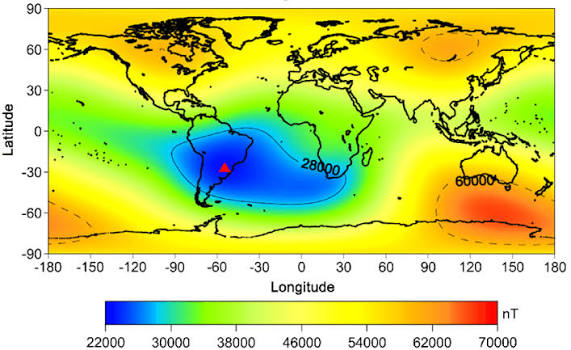
\includegraphics[width=\linewidth,height=0.65\textheight,keepaspectratio]{./media/saa_magnetic_anomaly.png}
\caption{South Atlantic Magnetic Anomaly (year 2000; source image from original draft).}\label{fig:saa-background}
\end{figure}

Although several trapped-radiation models such as AP8 and AP9 currently
exist, substantial uncertainties remain regarding temporal proton-flux
variability, storm-time behavior, directional anisotropies, and
localized radiation structures within the SAA. Existing models are
primarily statistical and often lack sufficient real-time data required
for modern small-satellite missions and future radiation-aware
spacecraft operations.

The ANTARA mission seeks to contribute toward closing these gaps through
direct in-situ measurement of high-energy proton populations using a
dedicated CubeSat operating in a Sun-Synchronous Orbit. The project also
enables students to gain practical experience in CubeSat designing and
modelling.


\subsubsection{Educational Motive}\label{educational-motive}One of the primary motivations behind ANTARA is the creation of an
educational and research platform capable of providing hands-on
experience in real-world spacecraft development.

The mission enables participating students to experience all major
phases of aerospace project development. Unlike isolated academic
laboratory experiments, CubeSat missions introduce students to highly
constrained engineering environments where mass, power, thermal limits
and others interact simultaneously. This systems-level complexity is one
of the most important educational benefits of the ANTARA mission.

\subsubsection{Scientific Motive}\label{scientific-motive}The primary scientific motivation behind ANTARA is the need for improved
understanding of the trapped proton environment within the South
Atlantic Anomaly and its implications for spacecraft operations,
radiation modelling, and near-Earth space science.

The South Atlantic Anomaly represents the region where the inner Van
Allen radiation belt approaches closest to Earth due to the offset and
tilt of Earth's magnetic dipole. Spacecraft traversing this region are
exposed to significantly elevated fluxes of energetic charged particles,
particularly high-energy protons capable of producing Single Event
Upsets (SEUs), sensor noise, detector saturation, memory corruption,
semiconductor degradation, and cumulative radiation damage.

ANTARA aims to contribute toward this scientific need by directly
measuring Unidirectional Differential Proton Flux (FPDU) within the
energy range of 5 MeV to 100 MeV using an onboard proton detection
payload. The mission seeks to generate spatially and temporally
correlated radiation datasets that can be compared against existing
radiation models including AP8 and AP9.

\subsubsection{National Motive}\label{national-motive}From a national perspective, ANTARA aligns strongly with India's growing
emphasis on indigenous space technology development, scientific
self-reliance, and advanced research capability. The mission contributes
toward India's requirement for indigenous expertise in spacecraft
systems engineering, radiation-aware electronics, mission operations,
and advanced satellite technologies.

Also, the satellites in the past few years have faced various anomalies
with this region due to which communication signals with them were lost.
Data collected by ANTARA maps the shifting borders of the SAA, allowing
Indian satellites to shield or power down domestic defense and
communication satellites before they sustain damage. ANTARA provides an
opportunity for low-cost effective and indigenous space tech to be
tested via its CubeSat.


\subsection{Mission Significance}\label{mission-significance}

\subsubsection{Primary Flight Objective}\label{primary-flight-objectives}
The primary objective is to measure and map unidirectional differential proton flux in the South Atlantic Anomaly over the 5--100~MeV range.

\subsubsection{Secondary Mission Objectives}\label{b.-secondary-mission-objectives}
The secondary objectives are to examine East--West asymmetry, characterize the bifurcation of the SAA, investigate atmospheric-loss coupling, and develop corrections to radiation-model predictions from ANTARA measurements. Storm-time comparisons remain an exploratory objective dependent on available observations. The detector architecture and channel definition remain under development; the science-success criteria are proposed targets to be tested against actual detection and sampling capability.

\subsection{Mission Success Criteria}\label{mission-success-criteria}

Mission success criteria define the measurable conditions under which
the ANTARA mission can be considered operationally and scientifically
successful. These criteria establish a structured framework for
evaluating mission performance at different levels of achievement
throughout the mission lifecycle. The criteria are divided into three
progressive categories:

\begin{itemize}
\item
  Minimum Mission Success (MMSC)
\item
  Full Mission Success (MSC)
\item
  Extended Mission Success (EMSC)
\end{itemize}

\subsubsection{Minimum Mission Success Criteria (MMSC)}\label{minimum-mission-success-criteria-mmsc}The MMSC defines the lowest acceptable bar for declaring the mission a
scientific and engineering success. Meeting the MMSC demonstrates that
ANTARA has survived launch, commissioned its payload, operated within
the SAA environment, and produced scientifically interpretable,
calibrated flux data at coarse spatial resolution.


\begin{longtable}{@{}
  >{\raggedright\arraybackslash}p{(\columnwidth - 2\tabcolsep) * \real{0.3349}}
  >{\raggedright\arraybackslash}p{(\columnwidth - 2\tabcolsep) * \real{0.6651}}@{}}
\caption{MMSC mission duration targets}\label{tab:01-mission-context-1}\\
\toprule\noalign{}
\textbf{Parameter} & \textbf{Target} \\
Mission duration & 4-6 Months minimum \\
Orbital count & 1750 orbits (4 months) to 2650 orbits (6 months) \\
SAA transit count & 700 to 1050 SAA transits across the mission duration \\
Minimum SAA passes for MMSC science & ≥ 150 passes with payload operational and telemetry received \\
\midrule\noalign{}
\endhead
\bottomrule\noalign{}
\endlastfoot
\end{longtable}

\begin{longtable}{@{}
  >{\raggedright\arraybackslash}p{(\columnwidth - 2\tabcolsep) * \real{0.3333}}
  >{\raggedright\arraybackslash}p{(\columnwidth - 2\tabcolsep) * \real{0.6667}}@{}}
\caption{MMSC spatial mapping requirements}\label{tab:01-mission-context-2}\\
\toprule\noalign{}
\textbf{Parameter} & \textbf{Value} \\
Grid resolution & 5° × 5° in geographic latitude and longitude \\
SAA region & Approved count-rate polygon; vertices in the coverage contract \\
Geometric polygon-overlap cells & 92; science eligibility requires validation \\
Cell dwell time per pass & \textasciitilde74 seconds per 5° latitude band at 7.5 km/s \\
\midrule\noalign{}
\endhead
\bottomrule\noalign{}
\endlastfoot
\end{longtable}

\begin{longtable}{@{}
  >{\raggedright\arraybackslash}p{(\columnwidth - 2\tabcolsep) * \real{0.2350}}
  >{\raggedright\arraybackslash}p{(\columnwidth - 2\tabcolsep) * \real{0.7650}}@{}}
\caption{MMSC science requirements}\label{tab:01-mission-context-3}\\
\toprule\noalign{}
\textbf{ID} & \textbf{Requirement} \\
MM-M-01 REQUIRED & The mission shall produce a calibrated 5°×5° flux map covering at least
70\% of grid cells within the approved SAA polygon with valid measurements
(≥3 independent SAA passes per cell). \\
MM-M-02 REQUIRED & Coverage shall include the SAA flux core (centred approximately on
310°E, 30°S) to ≥90\% even if peripheral cells fall below the 70\%
global threshold. \\
MM-M-03 REQUIRED & Each populated spatial cell shall report a calibrated differential
proton flux value in units of particles/cm²/s/sr/MeV for each
operational energy channel. \\
MM-M-04 REQUIRED & σ\_F/F ≤ 50\% per cell per channel. Requires approximately N ≥ 4 counts
per cell per channel. \\
MM-M-05 REQUIRED & Flux maps shall be produced for a minimum of 2 energy channels
independently. \\
\midrule\noalign{}
\endhead
\bottomrule\noalign{}
\endlastfoot
\end{longtable}


\textbf{MMSC Scientific Deliverables}

\begin{itemize}
\item
  Calibrated 5°×5° differential proton flux map in at least 2 energy
  channels
\item
  Flux uncertainty map (σ\_F/F per cell per channel)
\item
  Pass-count coverage map (N\_passes per spatial cell)
\item
  Detector performance report: channel stability, livetime fractions,
  dead-time characterisation
\item
  model-baseline comparison plots with residual map at 5° resolution
\item
  Mission timeline with all anomaly flags and excluded data intervals
  documented
\end{itemize}

\subsubsection{Mission Success Criteria (MSC)}\label{mission-success-criteria-msc}\begin{longtable}{@{}
  >{\raggedright\arraybackslash}p{(\columnwidth - 2\tabcolsep) * \real{0.3333}}
  >{\raggedright\arraybackslash}p{(\columnwidth - 2\tabcolsep) * \real{0.6667}}@{}}
\caption{MSC mission duration targets}\label{tab:01-mission-context-4}\\
\toprule\noalign{}
\textbf{Parameter} & \textbf{Value} \\
Required duration & 12 months - 14 months minimum \\
Orbital count & 5400 orbits (12 months) to 6300 orbits (14 months) \\
SAA transit count & 2150 to 2500 SAA transits \\
Minimum SAA passes for MSC science & ≥ 900 passes with payload operational \\
\midrule\noalign{}
\endhead
\bottomrule\noalign{}
\endlastfoot
\end{longtable}

\begin{longtable}{@{}
  >{\raggedright\arraybackslash}p{(\columnwidth - 2\tabcolsep) * \real{0.3333}}
  >{\raggedright\arraybackslash}p{(\columnwidth - 2\tabcolsep) * \real{0.6667}}@{}}
\caption{MSC spatial mapping requirements}\label{tab:01-mission-context-5}\\
\toprule\noalign{}
\textbf{Parameter} & \textbf{Value} \\
Grid resolution & 1° × 1° in geographic latitude and longitude \\
Geometric polygon-overlap cells & 2,020; science eligibility requires validation \\
Cell dwell time per pass & 15 seconds per 1° latitude band at 7.5 km/s \\
\midrule\noalign{}
\endhead
\bottomrule\noalign{}
\endlastfoot
\end{longtable}

\begin{longtable}{@{}
  >{\raggedright\arraybackslash}p{(\columnwidth - 2\tabcolsep) * \real{0.2350}}
  >{\raggedright\arraybackslash}p{(\columnwidth - 2\tabcolsep) * \real{0.7650}}@{}}
\caption{MSC science requirements}\label{tab:01-mission-context-6}\\
\toprule\noalign{}
\textbf{ID} & \textbf{Requirement} \\
MS-M-01 REQUIRED & The mission shall produce a calibrated 1°×1° flux map covering at least
90\% of approved SAA polygon cells that contain detectable flux. \\
MS-M-02 REQUIRED & Each populated 1°×1° cell shall achieve σ\_F/F ≤ 25\% in at least the
two lowest-energy operational channels. Requires N ≥ 16 counts per cell
per channel. \\
MS-M-03 REQUIRED & Independent flux maps for all operational energy channels, co-registered
on the same 1°×1° grid, released as a unified multi-band atlas. \\
MS-M-04 REQUIRED & Minimum of 5 independent SAA passes per populated cell for inclusion in
primary science map. \\
MS-M-05 REQUIRED & Monthly-averaged sub-maps produced and compared. Month-to-month
variation exceeding 3σ in any cell shall be flagged. \\
\midrule\noalign{}
\endhead
\bottomrule\noalign{}
\endlastfoot
\end{longtable}

\textbf{MSC Scientific Deliverables}

\begin{itemize}
\item
  1°×1° multi-channel calibrated differential proton flux atlas (primary
  science product)
\item
  Per-channel uncertainty maps at 1° resolution
\item
  radiation-model residual maps per energy channel
\item
  East-west asymmetry map with statistical significance per cell
\item
  Monthly sub-maps (12--14 monthly averages) for temporal trend analysis
\item
  Full public data release: calibrated counts, flux products, metadata,
  and uncertainty estimates
\end{itemize}

\subsubsection{Extended Mission Success Criteria (EMSC)}\label{extended-mission-success-criteria-emsc}\begin{longtable}{@{}
  >{\raggedright\arraybackslash}p{(\columnwidth - 2\tabcolsep) * \real{0.3333}}
  >{\raggedright\arraybackslash}p{(\columnwidth - 2\tabcolsep) * \real{0.6667}}@{}}
\caption{EMSC mission duration targets}\label{tab:01-mission-context-7}\\
\toprule\noalign{}
\textbf{Parameter} & \textbf{Value} \\
Required duration & 18 months minimum - 20 months nominal \\
Orbital count & 8100 orbits (18 months) to 9000 orbits (20 months) \\
SAA transit count & 3200 to 3600 SAA transits \\
Minimum SAA passes for EMSC science & ≥ 2400 passes with payload operational \\
\midrule\noalign{}
\endhead
\bottomrule\noalign{}
\endlastfoot
\end{longtable}

\begin{longtable}{@{}
  >{\raggedright\arraybackslash}p{(\columnwidth - 2\tabcolsep) * \real{0.3333}}
  >{\raggedright\arraybackslash}p{(\columnwidth - 2\tabcolsep) * \real{0.6667}}@{}}
\caption{EMSC spatial mapping requirements}\label{tab:01-mission-context-8}\\
\toprule\noalign{}
\textbf{Parameter} & \textbf{Value} \\
Grid resolution & 0.5° × 0.5° in geographic latitude and longitude \\
Geometric polygon-overlap cells & 7,940; science eligibility requires validation \\
Cell dwell time per pass & \textasciitilde7 seconds per 0.5° latitude band at orbital velocity \\
\midrule\noalign{}
\endhead
\bottomrule\noalign{}
\endlastfoot
\end{longtable}

\begin{longtable}{@{}
  >{\raggedright\arraybackslash}p{(\columnwidth - 2\tabcolsep) * \real{0.2350}}
  >{\raggedright\arraybackslash}p{(\columnwidth - 2\tabcolsep) * \real{0.7650}}@{}}
\caption{EMSC science requirements}\label{tab:01-mission-context-9}\\
\toprule\noalign{}
\textbf{ID} & \textbf{Requirement} \\
EM-M-01 REQUIRED & The mission shall produce a calibrated 0.5°×0.5° flux map. Primary
science map includes all cells where σ\_F/F ≤ 15\%. \\
EM-M-02 REQUIRED & ≥95\% coverage of cells where AP9 predicts flux exceeding 1\% of the
mission peak flux. \\
EM-M-03 REQUIRED & σ\_F/F ≤ 10\% in at least one energy channel per cell, and ≤ 15\% in all
other operational channels. \\
EM-M-04 REQUIRED & Minimum of 5 independent SAA passes per primary-map cell. \\
EM-M-05 REQUIRED & 0.5° map produced for each operational energy channel independently;
minimum 3 channels. \\
EM-M-06 REQUIRED & Final 0.5° science map produced as a time-integrated product over full
EMSC window, plus two 9--10 month sub-period maps. \\
\midrule\noalign{}
\endhead
\bottomrule\noalign{}
\endlastfoot
\end{longtable}


\begin{longtable}{@{}
  >{\raggedright\arraybackslash}p{(\columnwidth - 6\tabcolsep) * \real{0.2400}}
  >{\raggedright\arraybackslash}p{(\columnwidth - 6\tabcolsep) * \real{0.2492}}
  >{\raggedright\arraybackslash}p{(\columnwidth - 6\tabcolsep) * \real{0.2431}}
  >{\raggedright\arraybackslash}p{(\columnwidth - 6\tabcolsep) * \real{0.2677}}@{}}
\caption{Comparison of success tiers}\label{tab:01-mission-context-10}\\
\toprule\noalign{}
\textbf{Parameter} & \textbf{MMSC} & \textbf{MSC} & \textbf{EMSC} \\
Mission Duration & 4--6 months & 12--14 months & 18--20 months \\
Min SAA Passes & ≥ 150 & ≥ 900 & ≥ 2400 \\
Spatial Resolution & 5° × 5° & 1° × 1° & 0.5° × 0.5° \\
Geometric overlap cells & 92 & 2,020 & 7,940 \\
SAA Coverage & ≥ 70\% (≥90\% core) & ≥ 90\% & ≥ 95\% (primary) \\
σ\_F/F Threshold & ≤ 50\% & ≤ 25\% & ≤ 10--15\% \\
Min Passes/Cell & ≥ 3 & ≥ 5 & ≥ 5 \\
Energy Channels & ≥ 2 & ≥ 4 (all) & 3 sustained \\
AP9 Comparison & Basic ratio check & Full residual map (1°) & Sub-map residuals (0.5°) \\
\midrule\noalign{}
\endhead
\bottomrule\noalign{}
\endlastfoot
\end{longtable}



\subsection{Outstanding MCR Evidence}
\paragraph{Science verification path.} MMSC, MSC and EMSC are retained as committed requirements. Grid-cell occupancy, detector acceptance, energy migration and systematic uncertainty must be coupled with the chosen payload response before compliance can be claimed.

\paragraph{Coverage acceptance contract.} The polygon is the supplied count-rate domain, using east-positive longitude in $[-180,180)$ and positive-area cell overlap. Its geometric counts are not automatic science-success denominators. The coverage, pass, channel, precision and temporal requirements above remain committed. Eligible flux/core definitions and independent observation rules require acceptance before calculating compliance. Repeated samples in one visit are not independent passes. Counts require science-enabled exposure, qualified response/background and usable stored/downlinked products; pure Poisson thresholds alone do not establish calibrated flux precision.

\clearpage
\section{Mission Overview and Orbit Design}\label{sec:mission-overview}
The ANTARA mission has been conceived as a dedicated scientific CubeSat mission focused on characterizing the high-energy proton radiation environment within the South Atlantic Anomaly (SAA). The spacecraft is intended to operate in a near-circular Sun-Synchronous Low Earth Orbit. The detailed orbit propagation and trade-study results are provided in Appendix~\ref{app:orbit-rf} and Appendix~\ref{app:source-02}.

\subsection{Spacecraft Overview}\label{spacecraft-overview}
ANTARA is a 3U CubeSat with an on-board computer, an electrical power system, an attitude determination and control system, a communications system, and the scientific payload. The initial orbit is approximately 600~km at an inclination of $97.6^\circ$. No propulsion system is planned.

The mission design targets a spacecraft mass below 3~kg. The 4~kg upper allowance is not used as the spacecraft design limit. The component mass allocation, including the custom payload, will be closed using the bill of materials. The 3U spacecraft dimensions are approximately $100\times100\times340.5$~mm.

\subsection{Orbit Selection}\label{sec:orbit-design}
The preliminary orbit baseline is a 600~km Sun-Synchronous Orbit with an inclination of $97.6^\circ$ and an eccentricity of approximately 0.001. The latest seven-case RAAN power study reports its largest modeled mean generation at $180^\circ$; power and battery behavior depend on the insertion RAAN. ANTARA does not control the launch RAAN, so the spacecraft is being assessed across multiple RAAN cases. The approved future analysis epoch is 1 January 2029; the latest source-study CSVs must still be checked for epoch and configuration consistency.

\begin{table}[htbp]\centering
\caption{Preliminary orbit parameters}\label{tab:orbit-baseline}
\begin{tabularx}{\linewidth}{@{}lX@{}}\toprule
Parameter & Mission baseline / current status \\ \midrule
Initial altitude & Approximately 600~km \\
Inclination & $97.6^\circ$ \\
Eccentricity & Approximately 0.001 \\
RAAN & Launch-dependent; $0^\circ$ and $30^\circ$ are favorable cases, not requirements \\
Propulsion & None \\
\bottomrule\end{tabularx}\end{table}

The mission targets approximately five years of operational science. The newest long-term drag trade predicts approximately 8.2--10.0 years to its integration endpoint, generally around 300~km, under the assumptions of the supplied runs. One run stops above 300~km, and atmospheric reentry is not simulated. These are preliminary predictions, \emph{not} a demonstrated five-year deorbit lifetime or post-mission compliance assessment. Appendix~\ref{app:updated-raan} reports the detailed results and caveats.

\subsection{Mission Lifecycle}\label{sec:mission-lifecycle}
The mission is divided into Launch, Deployment, Cold and Dark, Detumbling, Commissioning, Nominal Operations, Extended Operations, and Mission End phases. Following deployment the spacecraft activates after the planned delay, enters Cold and Dark, performs detumbling, and proceeds toward power-positive operations and commissioning. Nominal operations consist of Sun Pointing, Detection, and Relay, with Safe Mode for recovery.

The extended phase begins after nominal mission objectives have been met. The minimum, full, and extended mission duration targets are defined in Section~\ref{mission-success-criteria}. The detailed phase descriptions and mode transitions are retained in Appendices~\ref{app:source-02} and~\ref{app:operational-logic}.

\subsection{Design Baseline and Open Decisions}\label{sec:design-baseline}
The orbit parameters above and the subsystem configurations in Section~\ref{spacecraft-architecture} are the current MCR baseline. The spacecraft design maximum is 3~kg and the approved analysis epoch is 1 January 2029. The launch RAAN is uncontrolled; final component mass allocations, payload dimensions and mission-consistent simulation configurations require confirmation. Where different simulation studies use different inputs, their results will remain associated with those inputs rather than being combined as one common spacecraft configuration.

\subsection{Outstanding MCR Evidence}
\paragraph{Orbit-study maturity.} The approved future analysis epoch is 1 January 2029. Historical-epoch orbit/RAAN outputs remain provisional engineering studies until regenerated. The five-year operational target is distinct from the new preliminary 8--10-year drag-to-cutoff predictions; neither a reentry date nor disposal compliance is verified. The previously inconsistent SAA-only-orbit statistic is withheld until its counter definition is repaired.

\clearpage
\section{Spacecraft Architecture and Ground Segment}\label{spacecraft-architecture}
The ANTARA spacecraft is a 3U CubeSat with the on-board computer as the main command and operations unit. The subsystem design currently uses preliminary COTS components along with the in-house scientific payload. Detailed specifications, operating estimates, and the original component tables are provided in Appendix~\ref{app:source-03}.

\paragraph{Requirement and evidence convention.} The tables below allocate existing mission objectives and interfaces; they do not replace Section~\ref{mission-success-criteria}. Status codes are S = SUPPORTED within the stated model/software scope, C = CONDITIONAL, O = OPEN, NM = NOT MET in the identified scenario, and NE = NOT EVALUATED. Supported does not mean flight-qualified. An OPEN DERIVED REQUIREMENT identifies an essential numerical allocation still to be established; missing concept-level limits are not automatically deferred to PDR. Exact parents, evidence paths and verification actions for every stable ID are in \path{docs/audit/SUBSYSTEM_REQUIREMENT_TRACEABILITY.md}.

\subsection{Electrical Power System (EPS)}\label{electrical-power-system-eps}
The spacecraft uses one fixed solar panel on the +Z face and two panels stowed on the -Y face that deploy toward the +Z direction. The mission power studies use a 25~Wh battery planning capacity. The proposed ISISPACE ICEPS2 Type A has a manufacturer-rated 28.8~Wh battery-pack configuration; the mission simulation is assessed at 25~Wh. The original RAAN trade study reports average generated power of 11.05~W and 11.40~W for $0^\circ$ and $30^\circ$ RAAN respectively. These are study-case predictions, not a guarantee at any launch RAAN. The power studies were performed using end-of-life assumptions; their margins require acceptance against an agreed common run baseline.

The EOL power simulations provide a provisional sizing basis. Solar active area, conversion losses and worst-case EOL margin must be explicitly tied to an approved simulation configuration before these results are reported as closed budgets (Appendix~\ref{app:detailed-budgets}).

% Generated from config/requirements/section3_feasibility_v1.json.
\begin{table}[H]\centering\small\setlength{\tabcolsep}{3pt}
\caption{Mission Feasibility Requirements: Electrical Power System (EPS)}\label{tab:fr-eps}
\begin{tabular}{@{}
>{\RaggedRight\arraybackslash}p{\dimexpr(\linewidth-8\tabcolsep)*13/100\relax}
>{\RaggedRight\arraybackslash}p{\dimexpr(\linewidth-8\tabcolsep)*42/100\relax}
>{\RaggedRight\arraybackslash}p{\dimexpr(\linewidth-8\tabcolsep)*13/100\relax}
>{\RaggedRight\arraybackslash}p{\dimexpr(\linewidth-8\tabcolsep)*23/100\relax}
>{\RaggedRight\arraybackslash}p{\dimexpr(\linewidth-8\tabcolsep)*9/100\relax}
@{}}
\toprule ID & Requirement / acceptance condition & Mission driver & Evidence / verification & Status\\\midrule
\phantomsection\label{req:ANT-EPS-FR-001}\mbox{ANT-EPS-}\newline\mbox{FR-001} & The EPS shall sustain the scheduled mission loads with the 25 Wh planning battery across representative launch-dependent RAAN and eclipse cases, without an accumulating energy deficit. & Energy / life & Corrected annual solar/load integrals are 50288.809/30866.103 Wh; runtime and EOL identity unresolved. \emph{Verify:} Analysis + test. & C\\
\addlinespace[3pt]
\phantomsection\label{req:ANT-EPS-FR-002}\mbox{ANT-EPS-}\newline\mbox{FR-002} & The EPS shall keep battery energy within selected-cell operating and depth-of-discharge limits during startup, science, Relay and Safe Mode. Numerical SOC/DoD limits remain OPEN DERIVED REQUIREMENTS. & Battery safety & Corrected annual minimum 15.097556 Wh; actual capacity and supplier limits unknown. \emph{Verify:} Analysis + test. & O\\
\addlinespace[3pt]
\phantomsection\label{req:ANT-EPS-FR-003}\mbox{ANT-EPS-}\newline\mbox{FR-003} & The EPS shall supply simultaneous and transient load demand within bus voltage, current and ripple allocations, including payload acquisition, radio transmit and actuator peaks. These limits remain OPEN DERIVED REQUIREMENTS. & Power interfaces & Mode loads exist; qualified peaks and bus limits absent. \emph{Verify:} Analysis + test. & O\\
\addlinespace[3pt]
\bottomrule
\end{tabular}
\end{table}
\begin{table}[H]\centering\small\setlength{\tabcolsep}{3pt}
\ContinuedFloat\captionsetup{list=no}
\caption{Mission Feasibility Requirements: Electrical Power System (EPS) (continued)}
\begin{tabular}{@{}
>{\RaggedRight\arraybackslash}p{\dimexpr(\linewidth-8\tabcolsep)*13/100\relax}
>{\RaggedRight\arraybackslash}p{\dimexpr(\linewidth-8\tabcolsep)*42/100\relax}
>{\RaggedRight\arraybackslash}p{\dimexpr(\linewidth-8\tabcolsep)*13/100\relax}
>{\RaggedRight\arraybackslash}p{\dimexpr(\linewidth-8\tabcolsep)*23/100\relax}
>{\RaggedRight\arraybackslash}p{\dimexpr(\linewidth-8\tabcolsep)*9/100\relax}
@{}}
\toprule ID & Requirement / acceptance condition & Mission driver & Evidence / verification & Status\\\midrule
\phantomsection\label{req:ANT-EPS-FR-004}\mbox{ANT-EPS-}\newline\mbox{FR-004} & The EPS shall generate the allocated Sun-Pointing energy using the fixed +Z panel and two deployed panels, with illumination, pointing and conversion losses explicitly accounted for. & Array / ADCS & Configuration defined; generating and deployed-area identities differ. \emph{Verify:} Analysis + test. & C\\
\addlinespace[3pt]
\phantomsection\label{req:ANT-EPS-FR-005}\mbox{ANT-EPS-}\newline\mbox{FR-005} & The EPS shall reserve energy for detumble, safe-state survival and recovery until the next usable generation opportunity; maximum recovery duration and energy reserve remain OPEN DERIVED REQUIREMENTS. & Startup / safety & One 2460 s detumble event; left-held load integral 1.528000 Wh; reserve not allocated. \emph{Verify:} Analysis + test. & O\\
\addlinespace[3pt]
\phantomsection\label{req:ANT-EPS-FR-006}\mbox{ANT-EPS-}\newline\mbox{FR-006} & The EPS shall maintain the mission energy allocation through the approximately five-year operations objective using traceable EOL degradation and cycling assumptions. & EOL / lifetime & EOL study inputs exist; average generation is not an EOL margin. \emph{Verify:} Analysis + test. & C\\
\addlinespace[3pt]
\bottomrule
\end{tabular}
\end{table}
\textit{Status: S supported within stated scope; C conditional; O open; NM not met; NE not evaluated.}
\paragraph{Feasibility assessment.} The array/battery architecture provides an analysis basis, not a closed margin. The 25 Wh planning value is not an allowed depth-of-discharge limit. Allocate startup reserve, bus peaks and worst-RAAN/EOL depletion at concept review; verify component aging and transients at PDR.


\subsection{Communications System (COMMS)}\label{communications-system-comms}
The preliminary communications system uses the GomSpace NanoCom AX100 and directional and omnidirectional spacecraft antennas. The planned primary ground station is at Goa; a crossed-Yagi ground antenna is being considered. Each visibility study retains its producing elevation mask; the historical contact export has no runtime mask manifest, while the candidate Science source defaults to $15^\circ$. No second mask correction is applied. A secondary station is an option if the primary station cannot support the required operations.

The preliminary communications assessment assumes an ideal gross downlink rate of 19.2 kbps during eligible ground-station relay windows, without an arbitrary throughput derating. This establishes an upper-bound modeled data-transfer opportunity rather than verified application-layer throughput. Detailed RF link-budget closure, protocol overhead, retransmission effects, and achievable net science-data throughput are deferred to PDR.

The MCR assumes 100\% science allocation during eligible Relay contact, or 2400 bytes/s. Detailed allocations and AX100 configuration remain PDR tasks. A 256~KiB dedicated science queue and 128~MiB persistent science allocation are preliminary candidates, not total OBC memory or demonstrated mission storage closure; see Appendix~\ref{app:science-data-budget}.

The preliminary communications assessment uses the full idealized 19.2 kbps gross transfer opportunity during eligible ground-station relay windows. No arbitrary link derating is imposed at MCR. Detailed RF link-budget closure, protocol overhead, packet losses, retransmissions, and achievable net payload throughput shall be assessed at PDR.

% Generated from config/requirements/section3_feasibility_v1.json.
\begin{table}[H]\centering\small\setlength{\tabcolsep}{3pt}
\caption{Mission Feasibility Requirements: Communications System (COMMS)}\label{tab:fr-com}
\begin{tabular}{@{}
>{\RaggedRight\arraybackslash}p{\dimexpr(\linewidth-8\tabcolsep)*13/100\relax}
>{\RaggedRight\arraybackslash}p{\dimexpr(\linewidth-8\tabcolsep)*42/100\relax}
>{\RaggedRight\arraybackslash}p{\dimexpr(\linewidth-8\tabcolsep)*13/100\relax}
>{\RaggedRight\arraybackslash}p{\dimexpr(\linewidth-8\tabcolsep)*23/100\relax}
>{\RaggedRight\arraybackslash}p{\dimexpr(\linewidth-8\tabcolsep)*9/100\relax}
@{}}
\toprule ID & Requirement / acceptance condition & Mission driver & Evidence / verification & Status\\\midrule
\phantomsection\label{req:ANT-COM-FR-001}\mbox{ANT-COM-}\newline\mbox{FR-001} & The communications planning budget shall use 19200 bit/s (2400 bytes/s), 100\% science allocation and no arbitrary derating during eligible visibility-intersect-Relay windows. & MCR link budget & Corrected annual Relay opportunity 428836800 bytes; full-rate arithmetic reproduced. \emph{Verify:} Analysis. & S\\
\addlinespace[3pt]
\phantomsection\label{req:ANT-COM-FR-002}\mbox{ANT-COM-}\newline\mbox{FR-002} & The communications schedule shall return the generated science workload within the accepted retention/outage envelope, with bounded backlog and no unaccounted science loss. The sustained workload/envelope remain OPEN DERIVED REQUIREMENTS. & Data balance & Corrected annual EMSC slot sensitivity:46637364 bytes; nominal peak75336 bytes; response/timing open. \emph{Verify:} Analysis + test. & C\\
\addlinespace[3pt]
\phantomsection\label{req:ANT-COM-FR-003}\mbox{ANT-COM-}\newline\mbox{FR-003} & The communications interface shall support BITS Goa with a traceable station, frequency/modem and elevation-mask configuration; capacity shall use the producing mask exactly once. & Ground interface & Historical station label GS1\_India; actual mask/RAAN unverified. \emph{Verify:} Analysis + test. & O\\
\addlinespace[3pt]
\bottomrule
\end{tabular}
\end{table}
\begin{table}[H]\centering\small\setlength{\tabcolsep}{3pt}
\ContinuedFloat\captionsetup{list=no}
\caption{Mission Feasibility Requirements: Communications System (COMMS) (continued)}
\begin{tabular}{@{}
>{\RaggedRight\arraybackslash}p{\dimexpr(\linewidth-8\tabcolsep)*13/100\relax}
>{\RaggedRight\arraybackslash}p{\dimexpr(\linewidth-8\tabcolsep)*42/100\relax}
>{\RaggedRight\arraybackslash}p{\dimexpr(\linewidth-8\tabcolsep)*13/100\relax}
>{\RaggedRight\arraybackslash}p{\dimexpr(\linewidth-8\tabcolsep)*23/100\relax}
>{\RaggedRight\arraybackslash}p{\dimexpr(\linewidth-8\tabcolsep)*9/100\relax}
@{}}
\toprule ID & Requirement / acceptance condition & Mission driver & Evidence / verification & Status\\\midrule
\phantomsection\label{req:ANT-COM-FR-004}\mbox{ANT-COM-}\newline\mbox{FR-004} & The communications protocol shall detect corrupted or missing records and resume interrupted transfers with identifiable sequence, acknowledgement and duplicate handling. & Transfer integrity & v3 CRC/sequence tested; packet reception and retry protocol absent. \emph{Verify:} Analysis + test. & O\\
\addlinespace[3pt]
\phantomsection\label{req:ANT-COM-FR-005}\mbox{ANT-COM-}\newline\mbox{FR-005} & The communications design shall close RF link and net science-throughput budgets for the selected hardware and operational geometry before claiming physical data-return compliance. & PDR RF closure & No qualified link margin or application throughput. \emph{Verify:} Analysis + hardware test. & NE\\
\addlinespace[3pt]
\bottomrule
\end{tabular}
\end{table}
\textit{Status: S supported within stated scope; C conditional; O open; NM not met; NE not evaluated.}
\paragraph{Feasibility assessment.} Histogram-based return and scheduled Relay are consistent with the current architecture. Full-rate capacity arithmetic is model-supported; sustained generation, matched contact identity and the outage envelope remain prerequisites to concept-level data balance. Physical link margin, protocol behavior and net throughput require PDR verification.


\subsection{Scientific Payload}\label{payload-subsystem}
The current FPDU concept uses five $6\times6\times14$~mm main scintillator blocks in series along X, plus one $6\times6\times2$~mm front scintillator. Particles enter the $+X$ face and travel inward toward $-X$. Main-block SiPMs attach to $\pm Y$ (ten sensors), with one further front SiPM: eleven total. Teflon coats $\pm Z$ at 0.11~mm per face, giving 6.22~mm coated Z dimension. EJ-550 grease provides optical coupling. These are \textbf{CONFIRMED DESIGN INPUT}; material, inter-block optical isolation and packaged CAD remain open. The historical silicon entrance is removed; a rear scintillator is optional and unselected. The proton-energy requirement remains 5--100~MeV.

The proposed chain is scintillator, SiPM, ASIC, ADC, MCU or FPGA, classification, reconstruction, 64-bin histogram, and storage/downlink. ASIC shaping is 20~ns. Coincidence-window references are 200~ns nominal, at least 250~ns including allowance, and approximately 300~ns preferred. A separate stated 20~ns post-shaping interval has unresolved meaning. Qualified dead time, ADC latency and processing latency remain unknown. MCU is preferred only if the entire architecture meets timing, throughput, buffering and power needs; no processor is selected.

The historical \textbf{PRELIMINARY ESTIMATE} of 400~Hz assumed protons only, 250~$\mu$m (0.25~mm) aluminium shielding, geometric factor 1~cm$^2$~sr and 100\% detection efficiency; its generating calculation remains unidentified. Supplied per-cell rates supersede that rounded estimate. Reproduced proton maxima are 358.920~Hz (mean) and 975.659~Hz (99th-percentile map), using isotropic conversion, $G=1$~cm$^2$~sr, unit efficiency and an integral threshold of 5.5~MeV. These 2026-01-01, 600~km maps are approved preliminary references for 2029 planning. Their rate script does not model shielding or accepted detector response. Electron rates also contribute to electronics design studies. Appendix~\ref{app:payload-detail} gives the full assumptions, diagrams, timing trade and data contract; actual maximum trigger throughput is unestablished.

Routine science uses the 292-byte Science Record v3: entry/exit timestamps, geographic position, 64 uint32 histogram bins, sequence, combined mode/health marker and CRC. Prefer three nonoverlapping readings per eligible cell visit, with fewer when actual acquisition timing permits; valid zero-count intervals are retained. No arbitrary minimum duration is imposed. Record validity, accumulated statistical precision and mission-tier success are separate. Table~\ref{tab:fpdu-telemetry} defines the reference encoding; radio framing is excluded.

% Generated from config/requirements/section3_feasibility_v1.json.
\begin{table}[H]\centering\small\setlength{\tabcolsep}{3pt}
\caption{Mission Feasibility Requirements: Scientific Payload}\label{tab:fr-pld}
\begin{tabular}{@{}
>{\RaggedRight\arraybackslash}p{\dimexpr(\linewidth-8\tabcolsep)*13/100\relax}
>{\RaggedRight\arraybackslash}p{\dimexpr(\linewidth-8\tabcolsep)*42/100\relax}
>{\RaggedRight\arraybackslash}p{\dimexpr(\linewidth-8\tabcolsep)*13/100\relax}
>{\RaggedRight\arraybackslash}p{\dimexpr(\linewidth-8\tabcolsep)*23/100\relax}
>{\RaggedRight\arraybackslash}p{\dimexpr(\linewidth-8\tabcolsep)*9/100\relax}
@{}}
\toprule ID & Requirement / acceptance condition & Mission driver & Evidence / verification & Status\\\midrule
\phantomsection\label{req:ANT-PLD-FR-001}\mbox{ANT-PLD-}\newline\mbox{FR-001} & The payload shall provide calibrated differential trapped-proton flux over 5–100 MeV, with energy-dependent response, background discrimination and uncertainty adequate for the approved tier products. & Proton science & No calibrated six-scintillator response; 5.4/5.5 MeV study cutoffs do not close 5 MeV. \emph{Verify:} Analysis + test. & O\\
\addlinespace[3pt]
\phantomsection\label{req:ANT-PLD-FR-002}\mbox{ANT-PLD-}\newline\mbox{FR-002} & The payload science chain shall enable a 5°×5° MMSC map: at least 70\% polygon coverage, 90\% core coverage, 3 independent passes/cell, at least 2 channels and fractional flux uncertainty ≤50\% per populated cell/channel. & MMSC & 92 geometric cells; eligible/core and independent-pass definitions unresolved. \emph{Verify:} Analysis + test. & O\\
\addlinespace[3pt]
\phantomsection\label{req:ANT-PLD-FR-003}\mbox{ANT-PLD-}\newline\mbox{FR-003} & The payload science chain shall enable the MSC 1°×1° atlas: at least 90\% detectable-cell coverage, 5 independent passes/cell, uncertainty ≤25\% in the two lowest operational channels, all operational channels, and monthly maps with >3σ changes flagged. & MSC & Detailed criteria say all operational channels; summary specifies ≥4. Both retained pending reconciliation. \emph{Verify:} Analysis + test. & O\\
\addlinespace[3pt]
\bottomrule
\end{tabular}
\end{table}
\begin{table}[H]\centering\small\setlength{\tabcolsep}{3pt}
\ContinuedFloat\captionsetup{list=no}
\caption{Mission Feasibility Requirements: Scientific Payload (continued)}
\begin{tabular}{@{}
>{\RaggedRight\arraybackslash}p{\dimexpr(\linewidth-8\tabcolsep)*13/100\relax}
>{\RaggedRight\arraybackslash}p{\dimexpr(\linewidth-8\tabcolsep)*42/100\relax}
>{\RaggedRight\arraybackslash}p{\dimexpr(\linewidth-8\tabcolsep)*13/100\relax}
>{\RaggedRight\arraybackslash}p{\dimexpr(\linewidth-8\tabcolsep)*23/100\relax}
>{\RaggedRight\arraybackslash}p{\dimexpr(\linewidth-8\tabcolsep)*9/100\relax}
@{}}
\toprule ID & Requirement / acceptance condition & Mission driver & Evidence / verification & Status\\\midrule
\phantomsection\label{req:ANT-PLD-FR-004}\mbox{ANT-PLD-}\newline\mbox{FR-004} & The payload science chain shall enable 0.5°×0.5° EMSC products: ≥95\% of cells above AP9 1\%-of-mission-peak eligibility, 5 independent passes/cell, ≥3 channels, ≤10\% uncertainty in one channel and ≤15\% in every other operational channel. & EMSC & Primary-map ≤15\% rule and two 9–10 month submaps remain binding; required-G percentiles are not compliance. \emph{Verify:} Analysis + test. & O\\
\addlinespace[3pt]
\phantomsection\label{req:ANT-PLD-FR-005}\mbox{ANT-PLD-}\newline\mbox{FR-005} & The payload mechanical/readout interface shall conform to five longitudinal 6×6×14 mm blocks, a 6×6×2 mm front element and eleven SiPMs, with no silicon entrance stage. & Approved FPDU & Geometry arithmetic/configuration checked; package/material/optics unselected. \emph{Verify:} Inspection + test. & C\\
\addlinespace[3pt]
\phantomsection\label{req:ANT-PLD-FR-006}\mbox{ANT-PLD-}\newline\mbox{FR-006} & The payload timing interface shall distinguish 20 ns ASIC shaping from the 200 ns coincidence target and ≥250 ns allowance (about 300 ns preferred); it shall not assign these values as detector dead time. & Timing / readout & Separate config fields; qualified latency/dead time remain unknown. \emph{Verify:} Analysis + test. & C\\
\addlinespace[3pt]
\bottomrule
\end{tabular}
\end{table}
\begin{table}[H]\centering\small\setlength{\tabcolsep}{3pt}
\ContinuedFloat\captionsetup{list=no}
\caption{Mission Feasibility Requirements: Scientific Payload (continued)}
\begin{tabular}{@{}
>{\RaggedRight\arraybackslash}p{\dimexpr(\linewidth-8\tabcolsep)*13/100\relax}
>{\RaggedRight\arraybackslash}p{\dimexpr(\linewidth-8\tabcolsep)*42/100\relax}
>{\RaggedRight\arraybackslash}p{\dimexpr(\linewidth-8\tabcolsep)*13/100\relax}
>{\RaggedRight\arraybackslash}p{\dimexpr(\linewidth-8\tabcolsep)*23/100\relax}
>{\RaggedRight\arraybackslash}p{\dimexpr(\linewidth-8\tabcolsep)*9/100\relax}
@{}}
\toprule ID & Requirement / acceptance condition & Mission driver & Evidence / verification & Status\\\midrule
\phantomsection\label{req:ANT-PLD-FR-007}\mbox{ANT-PLD-}\newline\mbox{FR-007} & The payload readout shall handle the declared mixed-species peak/burst trigger envelope without unflagged saturation, pileup, loss or counter overflow. Rate, loss and dead-time allocations remain OPEN DERIVED REQUIREMENTS. & All-particle throughput & Proton-only400 Hz is not a bound; electron incident proxies can dominate. \emph{Verify:} Analysis + test. & O\\
\addlinespace[3pt]
\phantomsection\label{req:ANT-PLD-FR-008}\mbox{ANT-PLD-}\newline\mbox{FR-008} & The payload response allocation shall provide energy-dependent effective geometric factor and livetime sufficient for tier exposure/precision, including background and reconstruction uncertainty. Required acceptance values remain conditional on verified exposure. & Acceptance / counts & Broad-band G95≈0.36–0.50 cm² sr at10\% is ideal counting arithmetic, not achieved G. \emph{Verify:} Analysis + test. & O\\
\addlinespace[3pt]
\phantomsection\label{req:ANT-PLD-FR-009}\mbox{ANT-PLD-}\newline\mbox{FR-009} & The payload science accounting shall conserve counts across acquisition time and effective energy-bin boundaries, retain valid zero-count exposure, and carry livetime, background and calibration identity into accumulated cell/channel uncertainty. & Scientific integrity & Reference conservation tests pass; legacy expected counts are not reconstructed events. \emph{Verify:} Analysis + test. & C\\
\addlinespace[3pt]
\bottomrule
\end{tabular}
\end{table}
\begin{table}[H]\centering\small\setlength{\tabcolsep}{3pt}
\ContinuedFloat\captionsetup{list=no}
\caption{Mission Feasibility Requirements: Scientific Payload (continued)}
\begin{tabular}{@{}
>{\RaggedRight\arraybackslash}p{\dimexpr(\linewidth-8\tabcolsep)*13/100\relax}
>{\RaggedRight\arraybackslash}p{\dimexpr(\linewidth-8\tabcolsep)*42/100\relax}
>{\RaggedRight\arraybackslash}p{\dimexpr(\linewidth-8\tabcolsep)*13/100\relax}
>{\RaggedRight\arraybackslash}p{\dimexpr(\linewidth-8\tabcolsep)*23/100\relax}
>{\RaggedRight\arraybackslash}p{\dimexpr(\linewidth-8\tabcolsep)*9/100\relax}
@{}}
\toprule ID & Requirement / acceptance condition & Mission driver & Evidence / verification & Status\\\midrule
\phantomsection\label{req:ANT-PLD-FR-010}\mbox{ANT-PLD-}\newline\mbox{FR-010} & The payload reference science format shall define entry/exit timestamps, latitude/longitude/altitude, 64 provisional uint32 bins, sequence, 16-bit mode/health marker and CRC in 292 bytes excluding radio framing. & Telemetry v3 & Codec/schema and CRC/count tests support the logical interface. \emph{Verify:} Inspection + software test. & S\\
\addlinespace[3pt]
\phantomsection\label{req:ANT-PLD-FR-011}\mbox{ANT-PLD-}\newline\mbox{FR-011} & The payload scheduler shall prefer 3 readings per eligible visit, seek 2 when feasible and retain 1 when necessary, with nonoverlapping valid intervals, correct cell assignment and conserved counts/exposure; no arbitrary minimum duration or count is imposed. & Reading policy & Reference partitions tested; exact crossings and hardware boundaries unknown. \emph{Verify:} Analysis + test. & C\\
\addlinespace[3pt]
\bottomrule
\end{tabular}
\end{table}
\textit{Status: S supported within stated scope; C conditional; O open; NM not met; NE not evaluated.}
\paragraph{Feasibility assessment.} The longitudinal scintillators and distributed SiPM readout define an inspectable payload concept; the record codec has bounded software evidence. Neither the stopping response nor effective geometric acceptance is calibrated. Material/optical interfaces, mixed-species trigger demand and qualified channels are concept-level feasibility gaps, not details that can be waived until qualification. The tier rows flow down Section 1 without replacing its criteria: MMSC uses at least two channels; MSC retains all operational channels and the comparison table's at-least-four statement pending reconciliation; EMSC retains its primary-map ≤15\% rule, minimum three channels and two 9–10 month sub-period maps. The counting examples N≈4 and N≥16 do not replace full uncertainty or create a new confidence level.


\subsection{Attitude Determination and Control System (ADCS)}\label{attitude-determination-and-control-system-adcs}
ANTARA intends to use an integrated reaction-wheel and magnetorquer attitude-control system; the earlier CMG description is superseded. The supplied TensorTech ADCS-10m databook describes a CMG-equipped unit and therefore does not confirm the intended reaction-wheel plus magnetorquer architecture. The ADCS vendor/product selection remains open. The main attitude functions are initial detumbling, Sun Pointing, payload +X pointing during SAA operations, +Y relay pointing toward the ground station, and Safe Mode recovery. Manufacturer limits and exact actuator configuration will be entered after the supplier data are reconciled with the selected model. The preliminary pointing goal remains subject to simulated and hardware verification. Mode transitions are given in Appendix~\ref{app:operational-logic}.

The supplied historical detumble summary contains 50\,000 trials, with 16\,133 reported successes (32.266\%). Successful trials alone have median completion 951.5~s and 95th percentile 2569.0~s. The 33\,867 nonconverged rows retain infinite completion values; their censor times and generating configuration are missing. All trials contain independently specified nonzero initial accelerations, which the current source rejects. These results therefore describe a historical synthetic model, not flight reliability or a qualified actuator envelope. The separate integrated startup event lasts 2460~s. Detailed interpretation is in Appendix~\ref{app:detumble-evidence}.

% Generated from config/requirements/section3_feasibility_v1.json.
\begin{table}[H]\centering\small\setlength{\tabcolsep}{3pt}
\caption{Mission Feasibility Requirements: Attitude Determination and Control System (ADCS)}\label{tab:fr-adcs}
\begin{tabular}{@{}
>{\RaggedRight\arraybackslash}p{\dimexpr(\linewidth-8\tabcolsep)*13/100\relax}
>{\RaggedRight\arraybackslash}p{\dimexpr(\linewidth-8\tabcolsep)*42/100\relax}
>{\RaggedRight\arraybackslash}p{\dimexpr(\linewidth-8\tabcolsep)*13/100\relax}
>{\RaggedRight\arraybackslash}p{\dimexpr(\linewidth-8\tabcolsep)*23/100\relax}
>{\RaggedRight\arraybackslash}p{\dimexpr(\linewidth-8\tabcolsep)*9/100\relax}
@{}}
\toprule ID & Requirement / acceptance condition & Mission driver & Evidence / verification & Status\\\midrule
\phantomsection\label{req:ANT-ADCS-FR-001}\mbox{ANT-ADCS-}\newline\mbox{FR-001} & The ADCS shall detumble and acquire a safe Sun-Pointing state from the accepted deployment attitude/rate envelope within the EPS startup allocation; envelope, deadline and reliability target remain OPEN DERIVED REQUIREMENTS. & Startup acquisition & One 2460 s event; historical 16133/50000 successes are source-incompatible. \emph{Verify:} Analysis + test. & O\\
\addlinespace[3pt]
\phantomsection\label{req:ANT-ADCS-FR-002}\mbox{ANT-ADCS-}\newline\mbox{FR-002} & The ADCS shall maintain payload +X science and +Y Relay boresights within allocated acceptance/link pointing-error envelopes during valid acquisition/transfer. Numeric error and jitter allocations remain OPEN DERIVED REQUIREMENTS. & Science / Relay pointing & No geometry-matched acceptance or selected-antenna error allocation. \emph{Verify:} Analysis + test. & O\\
\addlinespace[3pt]
\phantomsection\label{req:ANT-ADCS-FR-003}\mbox{ANT-ADCS-}\newline\mbox{FR-003} & The ADCS shall hold Sun Pointing and perform recovery/Safe Mode attitudes within the EPS generation and thermal allocations. Numeric attitude limits remain OPEN DERIVED REQUIREMENTS. & Survival pointing & Mode concept defined; common pointing-energy/thermal limits not closed. \emph{Verify:} Analysis + test. & O\\
\addlinespace[3pt]
\bottomrule
\end{tabular}
\end{table}
\begin{table}[H]\centering\small\setlength{\tabcolsep}{3pt}
\ContinuedFloat\captionsetup{list=no}
\caption{Mission Feasibility Requirements: Attitude Determination and Control System (ADCS) (continued)}
\begin{tabular}{@{}
>{\RaggedRight\arraybackslash}p{\dimexpr(\linewidth-8\tabcolsep)*13/100\relax}
>{\RaggedRight\arraybackslash}p{\dimexpr(\linewidth-8\tabcolsep)*42/100\relax}
>{\RaggedRight\arraybackslash}p{\dimexpr(\linewidth-8\tabcolsep)*13/100\relax}
>{\RaggedRight\arraybackslash}p{\dimexpr(\linewidth-8\tabcolsep)*23/100\relax}
>{\RaggedRight\arraybackslash}p{\dimexpr(\linewidth-8\tabcolsep)*9/100\relax}
@{}}
\toprule ID & Requirement / acceptance condition & Mission driver & Evidence / verification & Status\\\midrule
\phantomsection\label{req:ANT-ADCS-FR-004}\mbox{ANT-ADCS-}\newline\mbox{FR-004} & The ADCS shall complete and settle science/Relay slews before their qualified windows and keep transition overhead within the mission exposure/data-return allocation. Deadline and settling limits remain OPEN DERIVED REQUIREMENTS. & Slew timing & Complete day/year timestamp spans; telemetry/transition/slew duration definitions disagree. \emph{Verify:} Analysis + test. & O\\
\addlinespace[3pt]
\phantomsection\label{req:ANT-ADCS-FR-005}\mbox{ANT-ADCS-}\newline\mbox{FR-005} & The ADCS shall keep wheel momentum and torque within selected actuator limits and unload using magnetorquers against the declared disturbance envelope. Numerical authority/margin allocations remain OPEN DERIVED REQUIREMENTS. & Actuator authority & Hardware/field coupling unqualified; zero archived wheel momentum is not proof. \emph{Verify:} Analysis + test. & O\\
\addlinespace[3pt]
\phantomsection\label{req:ANT-ADCS-FR-006}\mbox{ANT-ADCS-}\newline\mbox{FR-006} & The ADCS shall report acquisition, saturation and pointing faults to the mode controller and enforce safe guards before declaring science/Relay readiness. & Mode reliability & FSM exists; historical boundary/SAFE timing discrepancies remain. \emph{Verify:} Simulation + hardware-in-loop. & C\\
\addlinespace[3pt]
\bottomrule
\end{tabular}
\end{table}
\textit{Status: S supported within stated scope; C conditional; O open; NM not met; NE not evaluated.}
\paragraph{Feasibility assessment.} Reaction wheels plus magnetorquers address controlled pointing and momentum unloading without reviving the CMG selection. The single startup event and incompatible Monte Carlo summary do not establish a detumble reliability. Initial-condition, pointing, torque and timing allocations must be justified at concept level; representative closed-loop and hardware-in-loop validation then belongs to PDR.


\subsection{On-Board Computer (OBC)}\label{on-board-computer-obc}
The source design uses the GomSpace NanoMind A3200 as the preliminary on-board computer. The OBC is responsible for mission sequencing, spacecraft state monitoring, command execution, payload control, data handling, and communications scheduling. The source document gives approximately 0.17~W as the average OBC power consumption for its stated operating conditions.

% Generated from config/requirements/section3_feasibility_v1.json.
\begin{table}[H]\centering\small\setlength{\tabcolsep}{3pt}
\caption{Mission Feasibility Requirements: On-Board Computer (OBC)}\label{tab:fr-obc}
\begin{tabular}{@{}
>{\RaggedRight\arraybackslash}p{\dimexpr(\linewidth-8\tabcolsep)*13/100\relax}
>{\RaggedRight\arraybackslash}p{\dimexpr(\linewidth-8\tabcolsep)*42/100\relax}
>{\RaggedRight\arraybackslash}p{\dimexpr(\linewidth-8\tabcolsep)*13/100\relax}
>{\RaggedRight\arraybackslash}p{\dimexpr(\linewidth-8\tabcolsep)*23/100\relax}
>{\RaggedRight\arraybackslash}p{\dimexpr(\linewidth-8\tabcolsep)*9/100\relax}
@{}}
\toprule ID & Requirement / acceptance condition & Mission driver & Evidence / verification & Status\\\midrule
\phantomsection\label{req:ANT-OBC-FR-001}\mbox{ANT-OBC-}\newline\mbox{FR-001} & The OBC shall allocate record assembly separately from the science queue: 292 bytes per packed reference record and explicitly budgeted acquisition banks, stack and DMA; a two-bank histogram fixture adds 512 bytes. & Assembly RAM & 804-byte illustrative payload working set; not total RAM or selected architecture. \emph{Verify:} Analysis + test. & C\\
\addlinespace[3pt]
\phantomsection\label{req:ANT-OBC-FR-002}\mbox{ANT-OBC-}\newline\mbox{FR-002} & The OBC science queue shall retain the corrected nominal workload without loss and provide nonvolatile spill for the accepted outage envelope; science RAM, persistent retention and total system memory shall be allocated separately. & Queue RAM & Corrected annual nominal EMSC peak75336 bytes; seven-day outage1010028 bytes exceeds256KiB RAM. \emph{Verify:} Analysis + software test. & C\\
\addlinespace[3pt]
\phantomsection\label{req:ANT-OBC-FR-003}\mbox{ANT-OBC-}\newline\mbox{FR-003} & The OBC persistent science store shall retain all unacknowledged records through the accepted contact-outage/retention envelope, including metadata/reserves; that envelope remains an OPEN DERIVED REQUIREMENT. & Persistent storage & Corrected annual seven-day EMSC outage peak1010028 bytes;128MiB exceeds it before reserves. \emph{Verify:} Analysis + test. & C\\
\addlinespace[3pt]
\bottomrule
\end{tabular}
\end{table}
\begin{table}[H]\centering\small\setlength{\tabcolsep}{3pt}
\ContinuedFloat\captionsetup{list=no}
\caption{Mission Feasibility Requirements: On-Board Computer (OBC) (continued)}
\begin{tabular}{@{}
>{\RaggedRight\arraybackslash}p{\dimexpr(\linewidth-8\tabcolsep)*13/100\relax}
>{\RaggedRight\arraybackslash}p{\dimexpr(\linewidth-8\tabcolsep)*42/100\relax}
>{\RaggedRight\arraybackslash}p{\dimexpr(\linewidth-8\tabcolsep)*13/100\relax}
>{\RaggedRight\arraybackslash}p{\dimexpr(\linewidth-8\tabcolsep)*23/100\relax}
>{\RaggedRight\arraybackslash}p{\dimexpr(\linewidth-8\tabcolsep)*9/100\relax}
@{}}
\toprule ID & Requirement / acceptance condition & Mission driver & Evidence / verification & Status\\\midrule
\phantomsection\label{req:ANT-OBC-FR-004}\mbox{ANT-OBC-}\newline\mbox{FR-004} & The OBC shall provision total FSW/system memory and execution capacity separately from record assembly, queue and persistent storage, covering control, reconstruction, commands and fault handling. Limits remain OPEN DERIVED REQUIREMENTS. & System RAM / compute & No integrated worst-case memory/execution budget. \emph{Verify:} Analysis + test. & O\\
\addlinespace[3pt]
\phantomsection\label{req:ANT-OBC-FR-005}\mbox{ANT-OBC-}\newline\mbox{FR-005} & The OBC shall maintain record integrity and sequence continuity across interrupted writes, reset and Relay interruption, recovering only complete records and retaining unacknowledged data. & Data persistence & Reference CRC passes; atomic media writes and acknowledgements not implemented. \emph{Verify:} Analysis + test. & NE\\
\addlinespace[3pt]
\phantomsection\label{req:ANT-OBC-FR-006}\mbox{ANT-OBC-}\newline\mbox{FR-006} & The OBC shall execute approved state-machine guards, validate commands, report faults and enter a defined safe state without uncommanded detector/Relay operation. & Control / fault management & Mode logic documented; flight integration and command integrity unqualified. \emph{Verify:} Analysis + test. & C\\
\addlinespace[3pt]
\bottomrule
\end{tabular}
\end{table}
\begin{table}[H]\centering\small\setlength{\tabcolsep}{3pt}
\ContinuedFloat\captionsetup{list=no}
\caption{Mission Feasibility Requirements: On-Board Computer (OBC) (continued)}
\begin{tabular}{@{}
>{\RaggedRight\arraybackslash}p{\dimexpr(\linewidth-8\tabcolsep)*13/100\relax}
>{\RaggedRight\arraybackslash}p{\dimexpr(\linewidth-8\tabcolsep)*42/100\relax}
>{\RaggedRight\arraybackslash}p{\dimexpr(\linewidth-8\tabcolsep)*13/100\relax}
>{\RaggedRight\arraybackslash}p{\dimexpr(\linewidth-8\tabcolsep)*23/100\relax}
>{\RaggedRight\arraybackslash}p{\dimexpr(\linewidth-8\tabcolsep)*9/100\relax}
@{}}
\toprule ID & Requirement / acceptance condition & Mission driver & Evidence / verification & Status\\\midrule
\phantomsection\label{req:ANT-OBC-FR-007}\mbox{ANT-OBC-}\newline\mbox{FR-007} & The OBC shall preserve payload timestamps, cell/configuration identity and linked livetime/background/quality metadata through storage and ground reconstruction, without treating unknown health as nominal. & Metadata / time & v3 has linked-session metadata; size/cadence and clock performance open. \emph{Verify:} Analysis + test. & O\\
\addlinespace[3pt]
\bottomrule
\end{tabular}
\end{table}
\textit{Status: S supported within stated scope; C conditional; O open; NM not met; NE not evaluated.}
\paragraph{Feasibility assessment.} The reference format makes the assembly and queue workloads concrete. A 256 KiB dedicated queue contains the corrected nominal sampled-gate workload; this is not a total OBC RAM requirement. The 128 MiB candidate store fails the separate 187498164-byte no-downlink grid-retention sensitivity, but that unmatched sensitivity is not an approved retention mission case. Sustained workload, outage policy and total system memory must be allocated before unconditional feasibility; media and reset tests follow at PDR.


\subsection{Spacecraft Coordinate System}\label{spacecraft-coordinate-system}
The spacecraft body frame uses +X as the RAM face and payload boresight, +Y as the directional antenna face, +Z as the fixed solar-panel face, -Y as the deployable-panel packed face, -Z as the omnidirectional communications antenna face, and -X as the deployment face.

% Generated from config/requirements/section3_feasibility_v1.json.
\begin{table}[H]\centering\small\setlength{\tabcolsep}{3pt}
\caption{Mission Feasibility Requirements: Spacecraft Coordinate System}\label{tab:fr-int}
\begin{tabular}{@{}
>{\RaggedRight\arraybackslash}p{\dimexpr(\linewidth-8\tabcolsep)*13/100\relax}
>{\RaggedRight\arraybackslash}p{\dimexpr(\linewidth-8\tabcolsep)*42/100\relax}
>{\RaggedRight\arraybackslash}p{\dimexpr(\linewidth-8\tabcolsep)*13/100\relax}
>{\RaggedRight\arraybackslash}p{\dimexpr(\linewidth-8\tabcolsep)*23/100\relax}
>{\RaggedRight\arraybackslash}p{\dimexpr(\linewidth-8\tabcolsep)*9/100\relax}
@{}}
\toprule ID & Requirement / acceptance condition & Mission driver & Evidence / verification & Status\\\midrule
\phantomsection\label{req:ANT-INT-FR-001}\mbox{ANT-INT-}\newline\mbox{FR-001} & The subsystem interface definitions shall preserve +X payload entrance with inward −X particle travel, ±Y main SiPMs, ±Z reflector faces, +Y relay boresight and +Z fixed-array orientation. & Body-frame ICD & Current config/diagrams agree; installation must be inspected. \emph{Verify:} Inspection + software test. & S\\
\addlinespace[3pt]
\phantomsection\label{req:ANT-INT-FR-002}\mbox{ANT-INT-}\newline\mbox{FR-002} & The navigation/time interface shall bound clock and position errors so each science interval is unambiguously assigned to its cell/exposure window. Numerical errors and synchronization allocations remain OPEN DERIVED REQUIREMENTS. & Spatial / temporal tags & Integer scaling and POSIX convention defined; actual accuracy unknown. \emph{Verify:} Analysis + test. & O\\
\addlinespace[3pt]
\phantomsection\label{req:ANT-INT-FR-003}\mbox{ANT-INT-}\newline\mbox{FR-003} & The integration ICD shall allocate power, harness/connector, data, thermal and safe-state interfaces with explicit ownership and compatible command/status semantics. & Subsystem interoperability & No closed common hardware/ICD baseline. \emph{Verify:} Analysis + test. & O\\
\addlinespace[3pt]
\bottomrule
\end{tabular}
\end{table}
\textit{Status: S supported within stated scope; C conditional; O open; NM not met; NE not evaluated.}
\paragraph{Feasibility assessment.} The common frame aligns payload, antenna and array interfaces and is supported as a documented convention only. Alignment tolerance, time/position accuracy and electrical/command ICD ownership remain open derived allocations. These interfaces must be defined before integrated margins can be combined; calibration and installation surveys verify them later.


\subsection{Thermal and Structural Configuration}\label{sec:thermal-architecture}
The supplied seven-node thermal history spans 24 hours of recorded labels. Independently reproduced internal-node extrema are $-14.061$ to $21.159^\circ$C; external-face extrema span $-25.958$ to $31.239^\circ$C. These are model predictions from one history with an independent synthetic heat schedule. The summary's hot/cold columns are this history's extrema, not separately verified bounding cases; its $\pm10^\circ$C allowance is not a demonstrated component margin. Actual case identity, node-to-component limits and DITL heat coupling remain open. Appendix~\ref{app:thermal-structural} presents the evidence. No structural or environmental qualification is implied.

% Generated from config/requirements/section3_feasibility_v1.json.
\begin{table}[H]\centering\small\setlength{\tabcolsep}{3pt}
\caption{Mission Feasibility Requirements: Thermal and Structural Configuration}\label{tab:fr-thermal_structural}
\begin{tabular}{@{}
>{\RaggedRight\arraybackslash}p{\dimexpr(\linewidth-8\tabcolsep)*13/100\relax}
>{\RaggedRight\arraybackslash}p{\dimexpr(\linewidth-8\tabcolsep)*42/100\relax}
>{\RaggedRight\arraybackslash}p{\dimexpr(\linewidth-8\tabcolsep)*13/100\relax}
>{\RaggedRight\arraybackslash}p{\dimexpr(\linewidth-8\tabcolsep)*23/100\relax}
>{\RaggedRight\arraybackslash}p{\dimexpr(\linewidth-8\tabcolsep)*9/100\relax}
@{}}
\toprule ID & Requirement / acceptance condition & Mission driver & Evidence / verification & Status\\\midrule
\phantomsection\label{req:ANT-THM-FR-001}\mbox{ANT-THM-}\newline\mbox{FR-001} & The thermal subsystem shall keep each selected component within traceable operating and survival temperature limits for nominal and Safe Mode cases; numerical limits/node mapping remain OPEN DERIVED REQUIREMENTS. & Component survival & One history: internal −14.061 to21.159°C; no component compliance limits. \emph{Verify:} Analysis + test. & O\\
\addlinespace[3pt]
\phantomsection\label{req:ANT-THM-FR-002}\mbox{ANT-THM-}\newline\mbox{FR-002} & The thermal assessment shall bound hot, cold and eclipse temperatures using mission-compatible attitude and mode-dependent internal heat loads, including startup, science, Relay and safe recovery. & Thermal cases & Supplied extrema are one history; 1.9–4.9 W schedule is independent of DITL. \emph{Verify:} Analysis + test. & C\\
\addlinespace[3pt]
\phantomsection\label{req:ANT-THM-FR-003}\mbox{ANT-THM-}\newline\mbox{FR-003} & The thermal interfaces shall allocate battery charge/discharge temperature constraints and payload temperature-dependent calibration/stability limits. Both numerical allocations remain OPEN DERIVED REQUIREMENTS. & Battery / calibration & No selected-part limits or payload thermal response characterization. \emph{Verify:} Analysis + test. & O\\
\addlinespace[3pt]
\bottomrule
\end{tabular}
\end{table}
\begin{table}[H]\centering\small\setlength{\tabcolsep}{3pt}
\ContinuedFloat\captionsetup{list=no}
\caption{Mission Feasibility Requirements: Thermal and Structural Configuration (continued)}
\begin{tabular}{@{}
>{\RaggedRight\arraybackslash}p{\dimexpr(\linewidth-8\tabcolsep)*13/100\relax}
>{\RaggedRight\arraybackslash}p{\dimexpr(\linewidth-8\tabcolsep)*42/100\relax}
>{\RaggedRight\arraybackslash}p{\dimexpr(\linewidth-8\tabcolsep)*13/100\relax}
>{\RaggedRight\arraybackslash}p{\dimexpr(\linewidth-8\tabcolsep)*23/100\relax}
>{\RaggedRight\arraybackslash}p{\dimexpr(\linewidth-8\tabcolsep)*9/100\relax}
@{}}
\toprule ID & Requirement / acceptance condition & Mission driver & Evidence / verification & Status\\\midrule
\phantomsection\label{req:ANT-THM-FR-004}\mbox{ANT-THM-}\newline\mbox{FR-004} & The thermal-mechanical design shall keep gradients and resulting distortions/stresses within allocated alignment and material limits; numerical limits remain OPEN DERIVED REQUIREMENTS. & Thermal gradients & 31.704°C face spread is a node difference, not structural stress. \emph{Verify:} Analysis + test. & O\\
\addlinespace[3pt]
\phantomsection\label{req:ANT-STR-FR-001}\mbox{ANT-STR-}\newline\mbox{FR-001} & The structure/integration budget shall fit the selected 3 U deployer envelope and keep the complete design mass, including all allocations and contingency, at or below 3.0 kg. & Envelope / mass & 1536.3 g is incomplete BOM; provider ICD, payload and deployment allocations open. \emph{Verify:} Analysis + test. & O\\
\addlinespace[3pt]
\phantomsection\label{req:ANT-STR-FR-002}\mbox{ANT-STR-}\newline\mbox{FR-002} & The structure shall withstand applicable launch loads and meet provider modal, vibration and shock requirements without loss of function or interface integrity. Numerical load/frequency limits remain OPEN DERIVED REQUIREMENTS. & Launch survival & No provider load envelope, FEA/modal or qualification evidence. \emph{Verify:} Analysis + test. & O\\
\addlinespace[3pt]
\bottomrule
\end{tabular}
\end{table}
\begin{table}[H]\centering\small\setlength{\tabcolsep}{3pt}
\ContinuedFloat\captionsetup{list=no}
\caption{Mission Feasibility Requirements: Thermal and Structural Configuration (continued)}
\begin{tabular}{@{}
>{\RaggedRight\arraybackslash}p{\dimexpr(\linewidth-8\tabcolsep)*13/100\relax}
>{\RaggedRight\arraybackslash}p{\dimexpr(\linewidth-8\tabcolsep)*42/100\relax}
>{\RaggedRight\arraybackslash}p{\dimexpr(\linewidth-8\tabcolsep)*13/100\relax}
>{\RaggedRight\arraybackslash}p{\dimexpr(\linewidth-8\tabcolsep)*23/100\relax}
>{\RaggedRight\arraybackslash}p{\dimexpr(\linewidth-8\tabcolsep)*9/100\relax}
@{}}
\toprule ID & Requirement / acceptance condition & Mission driver & Evidence / verification & Status\\\midrule
\phantomsection\label{req:ANT-STR-FR-003}\mbox{ANT-STR-}\newline\mbox{FR-003} & The solar deployment/retention mechanism shall retain both panels safely through launch and release/verify deployment without collision, harness damage or loss of the required generation geometry. & SDM / deployables & Architecture stated; mechanism, clearances and retention life unverified. \emph{Verify:} Analysis + test. & O\\
\addlinespace[3pt]
\phantomsection\label{req:ANT-STR-FR-004}\mbox{ANT-STR-}\newline\mbox{FR-004} & The mechanical integration shall preserve FPDU optical/readout interfaces and body-frame clearances through assembly, thermal cycling and operational life. & Payload packaging & Active material dimensions exclude coating, gaps, sensors and housing. \emph{Verify:} Analysis + test. & C\\
\addlinespace[3pt]
\bottomrule
\end{tabular}
\end{table}
\textit{Status: S supported within stated scope; C conditional; O open; NM not met; NE not evaluated.}
\paragraph{Feasibility assessment.} The lumped thermal model and 3U packaging are useful concept representations. They do not establish component thermal compliance or launch structural integrity. Missing selected-component limits, coupled hot/cold cases, complete mass and provider load/interface limits prevent an unconditional concept-feasibility finding. SDM/deployables remain here under the existing combined heading. Correlated thermal-vacuum, modal, vibration and deployment qualification are PDR verification tasks after those allocations exist.


\subsection{Ground Segment and Mission Operations}\label{ground-segment-mission-operations}
The primary ground station is planned at the Goa campus, approximately $15^\circ$N, $74^\circ$E. A second station is a contingency only if the primary station cannot meet operational requirements. The ground segment provides tracking, telemetry reception, commanding, and science-data retrieval. The operational sequence uses Cold and Dark, Detumble, Sun Pointing, Detection, Relay, and Safe Mode, with Slewing as an attitude-transition state in the simulation. The full state-machine logic is given in Appendix~\ref{app:operational-logic}.

% Generated from config/requirements/section3_feasibility_v1.json.
\begin{table}[H]\centering\small\setlength{\tabcolsep}{3pt}
\caption{Mission Feasibility Requirements: Ground Segment and Mission Operations}\label{tab:fr-gso}
\begin{tabular}{@{}
>{\RaggedRight\arraybackslash}p{\dimexpr(\linewidth-8\tabcolsep)*13/100\relax}
>{\RaggedRight\arraybackslash}p{\dimexpr(\linewidth-8\tabcolsep)*42/100\relax}
>{\RaggedRight\arraybackslash}p{\dimexpr(\linewidth-8\tabcolsep)*13/100\relax}
>{\RaggedRight\arraybackslash}p{\dimexpr(\linewidth-8\tabcolsep)*23/100\relax}
>{\RaggedRight\arraybackslash}p{\dimexpr(\linewidth-8\tabcolsep)*9/100\relax}
@{}}
\toprule ID & Requirement / acceptance condition & Mission driver & Evidence / verification & Status\\\midrule
\phantomsection\label{req:ANT-GSO-FR-001}\mbox{ANT-GSO-}\newline\mbox{FR-001} & The ground/operations chain shall plan and verify the approved observation windows: MMSC4–6 months and≥150 operational received passes; MSC12–14 months and≥900 operational passes; EMSC18–20 months and≥2400 operational passes. & Tier duration / passes & Corrected annual timestamp span complete; legacy response and source configuration not qualified. \emph{Verify:} Analysis + test. & O\\
\addlinespace[3pt]
\phantomsection\label{req:ANT-GSO-FR-002}\mbox{ANT-GSO-}\newline\mbox{FR-002} & Ground science processing shall reconstruct versioned cell/channel products from received records and linked exposure/calibration metadata, retaining zero counts, excluded-data reasons and independent-passage identifiers. & Map reconstruction & No received current-FPDU archive; reference codec is only a starting interface. \emph{Verify:} Analysis + test. & NE\\
\addlinespace[3pt]
\phantomsection\label{req:ANT-GSO-FR-003}\mbox{ANT-GSO-}\newline\mbox{FR-003} & Operations verification shall use complete, time-aligned telemetry, contact and transfer records for every claimed mission-window data-return result. & Evidence integrity & Corrected telemetry spans365days; contact/native data totals reconcile; mode/slew semantics unresolved. \emph{Verify:} Inspection + analysis. & C\\
\addlinespace[3pt]
\bottomrule
\end{tabular}
\end{table}
\begin{table}[H]\centering\small\setlength{\tabcolsep}{3pt}
\ContinuedFloat\captionsetup{list=no}
\caption{Mission Feasibility Requirements: Ground Segment and Mission Operations (continued)}
\begin{tabular}{@{}
>{\RaggedRight\arraybackslash}p{\dimexpr(\linewidth-8\tabcolsep)*13/100\relax}
>{\RaggedRight\arraybackslash}p{\dimexpr(\linewidth-8\tabcolsep)*42/100\relax}
>{\RaggedRight\arraybackslash}p{\dimexpr(\linewidth-8\tabcolsep)*13/100\relax}
>{\RaggedRight\arraybackslash}p{\dimexpr(\linewidth-8\tabcolsep)*23/100\relax}
>{\RaggedRight\arraybackslash}p{\dimexpr(\linewidth-8\tabcolsep)*9/100\relax}
@{}}
\toprule ID & Requirement / acceptance condition & Mission driver & Evidence / verification & Status\\\midrule
\phantomsection\label{req:ANT-GSO-FR-004}\mbox{ANT-GSO-}\newline\mbox{FR-004} & Ground operations shall establish primary-station availability and a missed-contact recovery schedule that maintains the accepted science retention envelope, including command/fault response. Availability and outage limits remain OPEN DERIVED REQUIREMENTS. & GS availability & Corrected longest intercontact gap48458s; actual station outage commitment unknown. \emph{Verify:} Analysis + test. & O\\
\addlinespace[3pt]
\bottomrule
\end{tabular}
\end{table}
\textit{Status: S supported within stated scope; C conditional; O open; NM not met; NE not evaluated.}
\paragraph{Feasibility assessment.} BITS Goa and the current mode sequence provide the planned operational path from exposure to received science. Historical contacts support opportunity calculations, not 2029 availability. Corrected annual timestamp coverage and contact/native data totals reconcile; transition and slew semantics remain unresolved. Observation eligibility, qualified independent passes and sustained station/outage assumptions must be closed at concept level; end-to-end exercises then verify the ground chain.


\subsection{Outstanding MCR Evidence}
\paragraph{Design maturity.} The MCR retains the reaction-wheel/magnetorquer architecture, selected solar-panel geometry and preliminary RF concept as a feasible spacecraft configuration. Detector response, finalized ADCS supplier interface, RF throughput and structural/thermal component compliance remain explicit PDR verification tasks rather than unspecified blanks.

% Generated from config/requirements/section3_feasibility_v1.json.
\begin{table}[H]\centering\small\setlength{\tabcolsep}{3pt}
\caption{Mission Feasibility Requirements: Outstanding MCR Evidence}\label{tab:fr-sys}
\begin{tabular}{@{}
>{\RaggedRight\arraybackslash}p{\dimexpr(\linewidth-8\tabcolsep)*13/100\relax}
>{\RaggedRight\arraybackslash}p{\dimexpr(\linewidth-8\tabcolsep)*42/100\relax}
>{\RaggedRight\arraybackslash}p{\dimexpr(\linewidth-8\tabcolsep)*13/100\relax}
>{\RaggedRight\arraybackslash}p{\dimexpr(\linewidth-8\tabcolsep)*23/100\relax}
>{\RaggedRight\arraybackslash}p{\dimexpr(\linewidth-8\tabcolsep)*9/100\relax}
@{}}
\toprule ID & Requirement / acceptance condition & Mission driver & Evidence / verification & Status\\\midrule
\phantomsection\label{req:ANT-SYS-FR-001}\mbox{ANT-SYS-}\newline\mbox{FR-001} & The system feasibility assessment shall identify a common mass, epoch, orbit/RAAN, duty-cycle, response and resource baseline for each combined margin and disclose incompatible evidence rather than pool it. & MCR integration & Existing studies differ in epoch/mass/response and completion. \emph{Verify:} Analysis + test. & C\\
\addlinespace[3pt]
\bottomrule
\end{tabular}
\end{table}
\textit{Status: S supported within stated scope; C conditional; O open; NM not met; NE not evaluated.}
\paragraph{Feasibility assessment.} The design-maturity statement above is conditional: missing essential allocations cannot all be deferred as detailed PDR work. Requirements marked S support only their stated reference/model scope; Corrected DITL evidence supersedes the prior annual truncation finding; logger/configuration closure remains conditional. The centralized register separates concept blockers from later qualification and records exact parents, interfaces and closure methods.


\clearpage
\section{Integrated Mission Feasibility}\label{sec:simulation-results}
The ANTARA simulation work combines orbit motion, power generation and consumption, attitude control, mode transitions, SAA operations, and ground-station contacts. This section gives the main results supported by the supplied historical study files. The detailed simulation descriptions, tables, and plots are retained in Appendices~\ref{app:source-04} and~\ref{app:sim-provenance}.

% Generated corrected-evidence block; see registry and audit.
\subsection{Day-in-the-Life Operations}\label{sec:sim-leop}
The corrected exports under \path{evidence/new-science-ditl/} replace the previously ingested incorrect/incomplete Science/DITL evidence. The old raw files, analyses and PDFs remain archived and must not support current numerical conclusions. The registry selects one source identity per scenario; no rows are pooled across runs. All three exports reach their named timestamp horizons: two 24-hour cases and one 365-day case. Absolute contact and SAA timestamps consistently identify 1 March 2000 UTC, not the approved 2029 analysis epoch.

The files contain no producing commit or runtime manifest. RAAN, mass, battery capacity, integrator, selected hardware and elevation mask therefore remain unverified. The two day cases have matching recorded orbital positions and contact windows to numerical precision, but complete configuration equivalence is not established. Their comparison is a sensitivity study, not a controlled causal test of LEOP alone.

The following telemetry integrals hold each recorded state over $[t_i,t_{i+1})$, exclude terminal-row duration, and sum to the recorded horizon. These exports lack explicit interval-end fields. Transition-log mode durations and slew-event durations are reported separately in Appendix~\ref{app:ditl-detail}; disagreements are not silently removed. Battery percentages elsewhere use 25 Wh only as an identified planning normalization, not a recovered capacity.
\begin{table}[H]\centering\small
\caption{Corrected telemetry accounting; left-held interval interpretation, historical epoch}\label{tab:annual-ditl}
\begin{tabularx}{\linewidth}{@{}Xrrr@{}}\toprule
Metric & LEOP 24 h & No-LEOP 24 h & LEOP 365 d\\\midrule
Recorded timestamp span (s) & 86,400 & 86,400 & 31,536,000\\
Sun Pointing (s) & 79,268 & 81,852 & 29,660,918\\
Detection (s) & 2,676 & 2,674 & 894,054\\
Relay (s) & 894 & 894 & 269,876\\
Slewing (s) & 980 & 980 & 375,688\\
Safe (s) & 0 & 0 & 332,882\\
Geographic SAA (s) & 2,696 & 2,696 & 881,882\\
Acquisition gate (s) & 758 & 758 & 247,258\\
Minimum recorded battery (Wh) & 15.128 & 18.004 & 15.098\\
Recorded solar integral (Wh) & 145.575 & 150.403 & 50,288.809\\
Recorded load integral (Wh) & 85.167 & 85.719 & 30,866.103\\
Native generation (source MB) & 0.009 & 0.009 & 3.514\\
Native transfer (source MB) & 0.009 & 0.009 & 3.514\\
\bottomrule\end{tabularx}\end{table}
\begin{figure}[H]\centering\includegraphics[width=\linewidth]{evidence/science-ditl/figures/corrected_20261109_day_occupancy_battery.png}
\caption{Corrected day-run mode occupancy and battery normalized to the 25 Wh planning reference. Same time span does not establish identical runtime configuration.}\label{fig:annual-mode-exposure}\end{figure}
Both day runs record 2,696 s geographic SAA dwell and 758 s acquisition gate. Removing startup does not increase this gate total in the supplied pair. LEOP includes one 2,460 s detumble event; this is not Monte Carlo reliability. For the annual trace, acquisition/SAA is 28.038\%, with numerator 247,258 s and denominator 881,882 s. Neither fraction is calibrated current-FPDU science duty.

Geographic SAA passages, sampled cell visits, gated exposure, model expected counts, accepted detector events and received science products are distinct. The legacy response does not qualify the six-scintillator FPDU. No MMSC/MSC/EMSC success percentage follows from these operational records.
\subsection{Ground Station and Data Return}\label{sec:sim-coverage}
The corrected annual contact log contains 820 intervals totaling 244,016 s. Mean daily contact is 668.537 s and minimum daily contact 514 s; the longest intercontact gap is 48,458 s. The source mask is unknown and is not applied a second time. Visibility alone corresponds to 585,638,400 bytes at 19.2 kbps. Intersecting these contacts with telemetry-labelled Relay yields 178,682 s, or 428,836,800 ideal bytes. Transition-log Relay instead gives 428,836,800 bytes; the timing-definition sensitivity remains explicit.

Native annual transfer credit is 3.514083862 source-labelled MB, separate from hypothetical v3 delivery. Source MB scaling and received-packet integrity are not demonstrated by the label. The v3 preferred EMSC workload generates 46,637,364 bytes with peak modeled queue 75,336 bytes and final backlog 0 bytes. It uses corrected, time-aligned sampled gates and Relay visibility at the full ideal 2400 bytes/s; it is not emitted v3 telemetry. Appendix~\ref{app:science-data-budget} gives tier and outage sensitivity.
The preliminary communications assessment uses the full idealized 19.2 kbps gross transfer opportunity during eligible ground-station relay windows. No arbitrary link derating is imposed at MCR. Detailed RF link-budget closure, protocol overhead, packet losses, retransmissions, and achievable net payload throughput shall be assessed at PDR.


\subsection{Updated RAAN Trade and Long-Duration Study}\label{sec:sim-annual}
The latest supplied RAAN campaign evaluates seven insertion cases from $0^\circ$ to $180^\circ$ in $30^\circ$ increments, with two runs per case. Average generated power varies from approximately 9.02~W ($120^\circ$) to 11.17~W ($180^\circ$), and tabulated mean of run-minimum battery SOC varies from approximately 54.4\% to 74.7\%. These are \emph{study-case outputs}, not a statement that the spacecraft can choose its insertion RAAN. Orbit classification totals are pooled across the two long-duration runs; they must not be mistaken for a one-year orbit tally. The full results, raw-count interpretation and drag-study limitations appear in Appendix~\ref{app:updated-raan}.

The drag CSV gives modeled termination times of roughly 8.2--10.0~years, generally near 300~km altitude. One case ends at 334.93~km, and none models final atmospheric reentry. The five-year \emph{science/operational objective} is therefore distinct from the provisional passive-decay estimate. The campaign configuration and epoch remain to be reconciled with the approved 1 January 2029, 3~kg mission baseline.

\subsection{Limitations of Current Evidence}\label{sec:sim-consolidated}
The corrected datasets replace the previous incomplete/incorrect Science exports. Full timestamp spans, matching contact durations and native data balances are established; exact producing source, runtime configuration, interval semantics and transition/slew reconciliation remain open. Legacy expected counts do not qualify current FPDU response, geographic eligibility, independent observations or science-tier success. The 2000 source epoch is retained. Independent RAAN, geometric-factor, radiation, thermal and detumble studies retain their own provenance and limitations; their assumptions are not pooled into one unconditional margin.

\clearpage
\section{Feasibility, Risk and Engineering Budgets}\label{mission-completion-requirements}
\subsection{Mission Feasibility}\label{sec:mission-feasibility}
The present MCR analysis supports the feasibility of a 3U spacecraft operating in a 600~km Sun-Synchronous Orbit with planned SAA detection and ground-station relay operations under the assumptions used in the source simulations. Final confirmation requires a common mass, power, payload, communications and ADCS baseline and the corresponding verified simulation results.

\subsection{Measures of Performance and Effectiveness}\label{measures-of-performance-mops}
The draft defines Measures of Performance (MOPs) for battery state of charge, Detection Mode pointing accuracy, science-data return, payload livetime and mission lifetime. Measures of Effectiveness (MOEs) address verified proton measurements, data return, radiation mapping and radiation-model comparison. Their original thresholds and goals are retained in Appendix~\ref{app:source-05} pending reconciliation with the final spacecraft configuration.

\subsection{Engineering Budgets}\label{sec:budget-closure}
The supplied bill of materials totals 1536.3~g for the rows with specified masses; this is not a complete spacecraft mass because the payload and deployment hardware are unallocated and the panel assembly quantity still requires checking. A design mass below 3~kg is targeted. Component costs are currently marked TBD. The payload and deployment hardware are not yet fully included in the mass total, and several component costs are still to be determined. The power analysis uses 25~Wh as the mission battery planning capacity; the proposed Type A datasheet gives 28.8~Wh rated. Final science-data rate and communications closure depend on payload decisions. The detailed component tables are retained in Appendix~\ref{app:source-05}, with reserved consolidated budgets in Appendix~\ref{app:detailed-budgets}.

\subsection{Risks and Requirements}\label{risk-method-and-register}
The draft identifies deployment failure, detumbling failure, loss of pointing, payload radiation damage, loss of communications, battery degradation and thermal excursion as mission risks. The original risk register does not yet provide complete likelihood and consequence scores. The requirements traceability matrix is preliminary and will need to be updated against the reorganized document and the final design values. Both source tables remain in Appendix~\ref{app:source-05}.

\subsection{End-of-Life and Debris Mitigation}\label{end-of-life-deorbit-and-debris-mitigation-compliance}
ANTARA does not carry propulsion and therefore relies on passive orbital decay for disposal. Its working operational science objective is approximately five years. The newly supplied long-term orbital-drag CSV reports modeled termination after approximately 8.2--10.0~years across seven RAAN cases and two runs per case; most traces end near 300~km, while one ends at approximately 335~km. This is a numerical propagation endpoint, not physical atmospheric reentry. A validated launch-epoch-specific drag model, final spacecraft aerodynamic properties, and subsequent atmospheric-decay assessment are required before making disposal-compliance claims. The full study is presented in Appendix~\ref{app:updated-raan}.

\subsection{MCR Open Items}\label{sec:open-issues}
Before the next review, the team must confirm the spacecraft mass and component baseline; reconcile the EPS energy capacity and electrical loads; finalize the ADCS actuator model and FPDU dimensions; validate the link and detector count assumptions; and connect each accepted simulation result to its source configuration. The supporting technical material is organized in the appendices.

\subsection{MCR Outcome and PDR Scope}\label{sec:mcr-pdr-scope}
The MCR establishes a preliminary mission baseline and examines the conditions under which the mission can be feasible using proposed COTS components and a custom payload. The final subsystem data paths, control paths, power distribution, communication implementation and payload design will be developed for the Preliminary Design Review (PDR). The present MCR should not be interpreted as completed hardware qualification or final selection of components whose interfaces and performance have not yet been verified.

\subsection{Outstanding MCR Evidence}
\paragraph{MCR decision and next review.} The MCR defines a conditionally feasible spacecraft concept with a maximum design mass of 3~kg. The detailed payload-electronics, data, ADCS control, power-distribution and RF interfaces are PDR design products. PDR entry requires traceable subsystem requirements, reconciled BOM, validation of the updated 8--10-year drag-to-cutoff study and a separate disposal assessment and measured or source-backed margins.

\paragraph{New evidence disposition.}
The corrected three-scenario evidence establishes complete named timestamp spans and reconciled native contact/data totals, superseding the old truncation finding. Runtime source/configuration and transition/slew semantics remain unresolved. Independent thermal component limits and detumble model/censoring records are still required. Current detector response, optics/electronics, actuator qualification, structural/thermal tests and RF net throughput remain open; no science-tier threshold changes.

\paragraph{Preliminary science-data handling.}
The 292-byte v3 record and three-reading preference remain unchanged. The corrected annual legacy-gate EMSC sensitivity generates 46637364 bytes, transfers that volume at full modeled 19.2 kbps, and peaks at 75336 bytes queued. This supports conditional data-handling feasibility for the sampled workload. A worst-start seven-day outage raises the required queue to 1010028 bytes: a 256 KiB RAM-only queue is insufficient for that case; nonvolatile spill is required. The 128 MiB candidate partition exceeds this modeled backlog before reserves, but sustained current-FPDU workload and retention remain unqualified. The separate geometric-grid archive is not mixed into this time-aligned annual run. Unknown logger/configuration identity and actual science response prevent unconditional mission closure.


% ==============================
% APPENDICES
% ==============================

\clearpage
\appendix

% Appendix A combines the six technical-support sections.
\section{Detailed Technical Supporting Analysis}
\label{app:technical-support}
\subsection{Detailed Operational Mode Transition Logic}\label{app:operational-logic}
The ANTARA concept of operations uses explicit spacecraft modes, bounded transition guards and a safety override. Figures~\ref{fig:op-transition-diagram} and~\ref{fig:op-mode-priorities} show the normal mission sequence and supervisory logic. The exact software thresholds are configuration-controlled simulation parameters, rather than independently qualified flight-software settings.

\subsubsection{Operational Modes and Attitude Targets}\label{app:op-logic-summary}
\begin{table}[htbp]\centering\footnotesize
\caption{Mode functions and commanding intent}\label{tab:op-mode-summary}
\begin{tabularx}{\linewidth}{@{}p{1.85cm}p{3.05cm}X@{}}\toprule
Mode & Attitude/control goal & Subsystem behavior and exit condition\\\midrule
Cold \& Dark & Deployment initialization; no operational pointing & Minimal EPS/OBC; initialize health monitoring and release startup delay; then Detumble.\\
Detumble & Reduce body rates using magnetic control & EPS/OBC/ADCS active; exit when rate and stability guard pass; otherwise remain or enter Safe on faults.\\
Sun Pointing & +Z solar face directed toward Sun & Default power-recovery and power-positive standby; permit scheduled SAA science or contact after safety guards.\\
Science / Detection & +X payload boresight aligned with required science pointing & Read out FPDU during a permitted SAA opportunity; account for payload warm-up, slew and available energy.\\
Relay / Downlink & +Y directional antenna aimed toward selected ground station & Radio TX/RX and queued-data transfer during usable elevation window; recover normal pointing after contact.\\
Passive / Eclipse & Preserve previous attitude during eclipse & Minimize active Sun-search maneuvers; resume Sun pointing or the applicable scheduled activity when illumination and guards permit.\\
Slewing & Move between required attitude targets & Temporary ADCS phase; next operational mode begins after reorientation/settling; abort on fault or low power.\\
Safe & Survival, battery conservation and anomaly handling & Suspend nonessential loads; maintain health, available communications and recovery control. Re-enter nominal path only after recovery guards.\\\bottomrule
\end{tabularx}\end{table}

\subsubsection{Nominal Startup and Science/Relay Sequence}\label{app:op-logic-diagram}
The sequence below extends the observed DITL behavior into a proposed operating procedure. It is an engineering interpretation for planning; the assumptions and their verification limits are stated after Section~\ref{app:op-logic-priority}.

\paragraph{Initialization and attitude acquisition.}
Following release, Cold \& Dark provides a protected initialization interval. The proposed sequence checks OBC boot status, time validity, EPS health and the availability of attitude sensors before enabling controlled acquisition. Deployment-related interlocks must be satisfied before an activity requiring deployed hardware is commanded; no additional deployment timing is assumed here. In the corrected LEOP event records, the startup delay is 120~s and detumbling occupies the following 2,460~s. Their sum, 2,580~s (43~min), is an event-defined reference for reaching the end of detumbling, not the time at which qualified science necessarily begins. The sampled Cold \& Dark occupancy is 122~s, so event endpoints and sampled mode durations must not be interchanged.

Detumbling is assumed to terminate on acceptable measured body rates and a stable attitude solution, rather than on expiry of the observed 2,460~s. The spacecraft then acquires Sun pointing, with the +Z solar face directed toward the Sun, to establish a power-recovery state and assess readiness for scheduled tasks. A failed acquisition remains an ADCS/recovery problem; it does not authorize blind continuation to Science. Neither a worst-case startup duration nor a deployment-success probability follows from the supplied LEOP examples.

\paragraph{Preparing and executing science.}
From Sun Pointing, the scheduler checks an approaching SAA opportunity against predicted slew/settling time, available energy and payload readiness. The intended +X payload pointing is acquired before measurement exposure is credited. A short opportunity may therefore be skipped or used only for its remaining valid interval. Geometric SAA residence alone is insufficient: the acquisition gate also requires instrument availability, valid pointing and acceptable health.

During acquisition, each histogram is attributed to one geographic cell and its own entry/exit timestamps. The preferred three readings per eligible visit use distinct intervals; two or one remain valid when timing or an interruption prevents three. No numerical minimum duration is imposed. A cell crossing, instrument shutdown or loss of acquisition validity closes the current interval. Valid zero-count records are retained, and partitioning a visit must conserve its counts and exposure. Multiple readings in one visit do not constitute independent orbital passages, and record validity does not imply that the cell/channel precision requirement is already satisfied.

\paragraph{Relay and return to standby.}
A scheduled BITS Goa opportunity permits a slew to the +Y antenna target only when the contact, attitude and resource guards are satisfied. Transfer is restricted to the intersection of visibility and Relay operation. The planning model offers the queued science data the full idealized 19.2~kbps during this intersection, without arbitrary derating; it does not demonstrate net hardware throughput. Contact termination or an override pauses delivery, preserving pending records for a later opportunity. The nominal sequence returns to Sun Pointing after a task, or transitions to another eligible task when its guards permit. In eclipse, retaining the previous attitude is a candidate low-activity fallback only while thermal, energy and attitude constraints allow it.

\begin{figure}[H]\centering
\resizebox{\linewidth}{!}{%
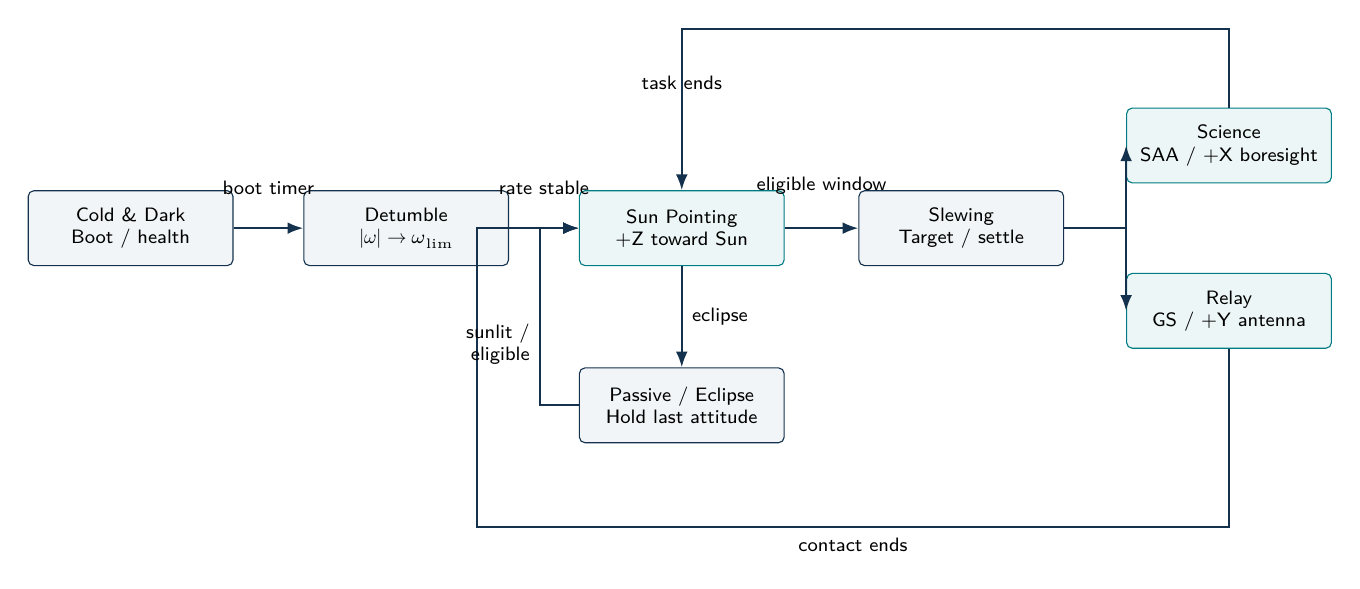
\begin{tikzpicture}[>=Latex,font=\sffamily\scriptsize,
 state/.style={draw=AntaraNavy,fill=AntaraPale,rounded corners=2pt,minimum width=2.6cm,minimum height=0.95cm,align=center},
 task/.style={state,draw=AntaraTeal,fill=AntaraTeal!7},
 flow/.style={-{Latex[length=2mm]},thick,draw=AntaraNavy}]
\node[state] (cold) at (0,0) {Cold \& Dark\\Boot / health};
\node[state] (det) at (3.5,0) {Detumble\\$|\boldsymbol\omega|\to\omega_{\rm lim}$};
\node[task] (sun) at (7.0,0) {Sun Pointing\\+Z toward Sun};
\node[state] (slew) at (10.55,0) {Slewing\\Target / settle};
\node[task] (science) at (13.95,1.05) {Science\\SAA / +X boresight};
\node[task] (relay) at (13.95,-1.05) {Relay\\GS / +Y antenna};
\node[state] (pass) at (7,-2.25) {Passive / Eclipse\\Hold last attitude};
\draw[flow] (cold)--node[above=3mm]{boot timer}(det);
\draw[flow] (det)--node[above=3mm]{rate stable}(sun);
\draw[flow] (sun)--node[above=3mm]{eligible window}(slew);
\draw[flow] (slew.east) -| (science.west);
\draw[flow] (slew.east) -| (relay.west);
\draw[flow] (science.north) -- ++(0,1) -| node[pos=.72,above]{task ends} (sun.north);
\draw[flow] (relay.south) -- (13.95,-3.8) -- node[below]{contact ends} (4.4,-3.8) -- (4.4,0) -- (sun.west);
\draw[flow] (sun.south)--node[right]{eclipse}(pass.north);
\draw[flow] (pass.west) -- (5.2,-2.25) -- node[left,align=right]{sunlit /\\eligible} (5.2,-0.7) -- (5.2,0) -- (sun.west);
\end{tikzpicture}}
\caption{Information-bearing functional flow of the planned mission sequence. Windows and guards come from the mission scheduler. The schematic does not assert that every transition is immediate; slew and settling times are accounted for separately.}\label{fig:op-transition-diagram}
\end{figure}

\subsubsection{Supervisory Priority and Safety Overrides}\label{app:op-logic-priority}
The supervisor evaluates spacecraft survival before granting any scheduled activity. The proposed policy separates a task that is temporarily ineligible from a condition requiring Safe mode. For example, an unavailable contact or unsettled pointing defers Relay or Science; a critical battery, thermal or control-state violation preempts the active task. The corrected annual run contains Safe-mode occupancy, but this alone does not establish which physical fault caused each entry or qualify the recovery guards.

\paragraph{Priority when opportunities overlap.}
Survival and recovery take precedence over science and downlink. Among otherwise admissible tasks, this planning interpretation uses the predicted consequences of deferral: loss of a scarce science window, queue overflow before the next contact, and the energy needed to execute and recover from a slew. Relay is not assumed universally superior to Science, nor is simultaneous acquisition and downlink credited. A deterministic scheduler must record the selected task and reason for deferral. Numerical priorities, queue watermarks and energy reserves remain to be allocated; the corrected exposure and backlog results constrain that trade but do not identify an optimal flight scheduler.

\paragraph{Interruption, safe state and recovery.}
On a critical override, the proposed response closes the valid acquisition interval, marks any uncertain data, inhibits nonessential payload/transmitter loads and preserves recoverable queue and sequence state. Health monitoring and feasible attitude control continue within the surviving power budget. Safe mode is therefore a fault-dependent operating state, not a promise of uninterrupted Sun pointing: excessive rates may first require Detumble, while a sensor fault may prevent the nominal attitude solution.

Recovery requires evidence that the initiating condition has cleared and that the intended next mode is admissible. Separate entry and recovery guards, with persistence checks where appropriate, are proposed to prevent repeated mode switching near a threshold. Their values are not inferred from sampling cadence. Recovery proceeds through Detumble if rate stabilization is needed, otherwise through Sun Pointing and readiness checks before science or relay resumes. Interrupted transfers require integrity and sequence reconciliation before records are retired from persistent storage; the final acknowledgement/retry protocol remains a PDR interface decision.

\begin{figure}[H]\centering
\resizebox{.94\linewidth}{!}{%
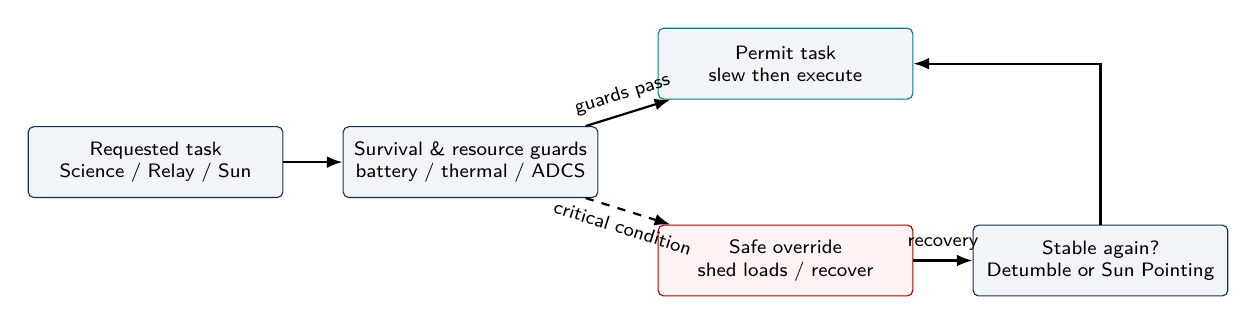
\begin{tikzpicture}[>=Latex,font=\sffamily\scriptsize,
 node/.style={draw=AntaraNavy,rounded corners=2pt,fill=AntaraPale,minimum height=9mm,text width=3cm,align=center},
 arr/.style={-{Latex[length=2mm]},thick}]
\node[node] (schedule) at (0,0) {Requested task\\Science / Relay / Sun};
\node[node] (guard) at (4,0) {Survival \& resource guards\\battery / thermal / ADCS};
\node[node,draw=AntaraTeal] (grant) at (8,1.25) {Permit task\\slew then execute};
\node[node,draw=red!65!black,fill=red!5] (safe) at (8,-1.25) {Safe override\\shed loads / recover};
\node[node] (resume) at (12,-1.25) {Stable again?\\Detumble or Sun Pointing};
\draw[arr] (schedule)--(guard);
\draw[arr] (guard)--node[above,sloped]{guards pass}(grant);
\draw[arr,dashed] (guard)--node[below,sloped]{critical condition}(safe);
\draw[arr] (safe)--node[above]{recovery}(resume);
\draw[arr] (resume.north) |- (grant.east);
\end{tikzpicture}}
\caption{Supervisory decision logic: survival constraints override scheduled science and downlink. Recovery transitions depend on the fault and attitude state; this is a mission-level policy, not an assertion of finalized flight code.}\label{fig:op-mode-priorities}
\end{figure}

\paragraph{Assumptions and extrapolation limits for A.1.2--A.1.3.}
The following assumptions make the proposed sequence explicit. They are not additional measured results or approved numerical flight-software settings. The evidence basis is the corrected LEOP/no-LEOP exports and annual run in Appendix~\ref{app:startup-evidence}, together with the current telemetry and communications contracts. Those runs use a historical 2000 epoch, and unresolved telemetry/event timing differences prevent treating this narrative as a reconstruction of every executed transition.
\begin{longtable}{@{}p{1.1cm}p{5.0cm}p{5.6cm}@{}}
\caption{Planning assumptions used to extend the operational sequence}\label{tab:op-sequence-assumptions}\\\toprule
ID & Assumed operating interpretation & Basis and required verification\\\midrule\endfirsthead
\toprule ID & Assumed operating interpretation & Basis and required verification\\\midrule\endhead
OP-A1 & Boot health/time checks and deployment interlocks precede dependent activities. & Necessary interface interpretation; individual checks are not demonstrated by the CSVs. Verify startup software, sensor readiness and deployment inhibits.\\
OP-A2 & Rate/attitude guards release Detumble; Sun Pointing provides the nominal recovery path. & Observed LEOP sequence supports the concept. The 43~min event reference is not a fixed timer or reliability bound; qualify guards and initial-condition coverage.\\
OP-A3 & Scheduling reserves time and energy for slew, settling and task recovery. & Logs contain slew and mode overhead, with differing timing semantics. Reconcile these and establish pointing, reserve and instrument-readiness allocations.\\
OP-A4 & Science and Relay compete for scheduled operation; deferral considers science opportunity and backlog. & Exclusive modeled modes and corrected queue studies motivate the trade. Verify arbitration, outage handling and any future concurrent-operation claim.\\
OP-A5 & Overrides preserve valid interval boundaries and recoverable record state. & Required by nonoverlapping v3 records and integrity objectives; power-loss atomicity and interrupted-transfer recovery are not demonstrated.\\
OP-A6 & Recovery uses fault clearance, persistence and distinct entry/exit guards. & Proposed protection against unstable switching. Set thresholds from component limits and control behavior, then exercise fault injection and repeated recovery.\\\bottomrule
\end{longtable}
These assumptions support a preliminary operational concept, not a quantitative guarantee of science yield, safe-mode endurance or communications reliability. Essential pointing, battery-reserve, thermal and readiness limits must be allocated before the sequence can demonstrate feasibility across the required operating cases; hardware tests and detailed implementation verification then close the PDR evidence.

\subsubsection{Transition and Guard Matrix}\label{app:op-logic-matrix}
\begin{longtable}{@{}p{2.25cm}p{2.55cm}p{6.9cm}@{}}
\caption{Required operational transitions and relevant checks}\label{tab:op-transition-matrix}\\\toprule
From & To & Guard / interpretation\\\midrule\endfirsthead\toprule From & To & Guard / interpretation\\\midrule\endhead
Cold \& Dark & Detumble & Boot/commissioning delay complete, EPS and OBC alive.\\
Detumble & Sun Pointing & Body rate falls below accepted rate threshold and attitude solution remains stable.\\
Sun Pointing & Slewing $\to$ Science & SAA opportunity exists, safe battery reserve and payload readiness; +X boresight target feasible.\\
Sun Pointing & Slewing $\to$ Relay & Ground contact above selected mask, queued data or command requirement, sufficient energy; +Y antenna acquisition.\\
Science & Sun Pointing / Relay & SAA window ends or a higher-priority valid contact is scheduled; use Slewing as needed.\\
Relay & Sun Pointing / Science & Contact ends, queue complete or higher-priority science becomes available; attitude guard applies.\\
Sun Pointing & Passive / Eclipse & Eclipse begins; passively retain last attitude rather than repeatedly Sun-searching.\\
Passive / Eclipse & Sun Pointing & Sun visibility returns and recovery/scheduling permits active pointing.\\
Any operational mode & Safe & Critical battery, ADCS, thermal or spacecraft health condition supersedes nominal task.\\
Safe & Detumble / Sun Pointing & Fault clearance and recovery guards satisfied; select Detumble if rates require stabilization.\\
Slewing & Scheduled target / Safe & Target within pointing/settling tolerance or slew interruption on fault/resource guard.\\\bottomrule\end{longtable}

\subsubsection{Timing, Power and Science Opportunity Accounting}\label{app:op-logic-accounting}
A useful SAA crossing is not automatically a valid measurement window. The data-taking interval is the portion of the crossing for which the payload is enabled, pointing has settled, coincidence acquisition is active and no resource/safety override applies. Equivalently,
\begin{equation}
T_{\rm science,usable}=\int_{t_0}^{t_1}\mathbf{1}_{\rm SAA}\,\mathbf{1}_{\rm payload}\,\mathbf{1}_{\rm pointing}\,\mathbf{1}_{\rm health}\,dt.
\end{equation}
The integrated logs distinguish transitions, slews, SAA passages, accepted proton events and ground-station contacts. The current one-year provisional output reports 2,346 SAA-passage records and 820 primary-station contact records. These are \emph{event-log counts for the supplied historical-epoch run}, not unique orbital revolutions or verified 2029 yields. A 2,460-second startup detumble event is observed in that run. These values are to be reconciled with the approved 2029 run before final MCR exit.

\subsubsection{Implementation Boundary}\label{app:op-logic-note}
The mode architecture, fault-preemption policy, Sun-pointing fallback and science/relay sequencing are MCR-level decisions. Exact battery-voltage thresholds, rate limits, thermal recovery timers, attitude-control gains, antenna acquisition tolerances and software task deadlines belong to the controlled ADCS/OBC configuration and must be verified at PDR. This section intentionally describes the complete concept and its verification boundary without claiming an untested flight implementation.

\subsubsection{Observed Startup Evidence}\label{app:startup-evidence}
The corrected exports include one 2460 s detumble event in each LEOP scenario, with initial rates $(6,-5.5,4.5)$ deg/s and accelerations $(0.12,-0.015,0.08)$ deg/s$^2$. No-LEOP has no detumble-event schema. This is not a verified deployment distribution. Corrected telemetry spans the complete named horizons, but transition timing and slew occupancy differ from event definitions; mode guards and recovery are not thereby qualified. All three corrected scenarios now participate in the evidence review; the prior exclusion of incomplete day exports is superseded.

\clearpage
\subsection{Detailed Scientific Payload: Approved FPDU Concept}\label{app:payload-detail}
The current source of truth is configuration \texttt{FPDU-2026-11-04-approved-v2}, referenced by \path{config/payload/current.json}. It supersedes the earlier same-day input snapshot and the single-block Rev.~2.1 narrative without claiming a formally released hardware revision. The mission requirement remains directional differential proton-flux measurement over 5--100~MeV. No geometry-matched detector response has yet qualified that interval.

\textbf{Evidence convention.} \textbf{CONFIRMED DESIGN INPUT} denotes approved construction or mission inputs; \textbf{PRELIMINARY ESTIMATE} denotes conditional planning assumptions; \textbf{MODEL PREDICTION} denotes a calculation under stated assumptions; \textbf{VALIDATED RESULT} is restricted to the tested software identity or arithmetic, not inferred hardware performance; \textbf{OPEN DECISION} denotes unresolved design choices. Detector response and hardware performance require validation.

\subsubsection{Geometry, Axes and Optical Interfaces}\label{app:payload-configuration}
\begin{table}[H]\centering\small
\caption{Confirmed FPDU mechanical inputs; dimensions exclude packaging}\label{tab:fpdu-design-summary}
\begin{tabularx}{\linewidth}{@{}p{3.1cm}p{4.1cm}X@{}}\toprule
Element & Current specification & Interpretation\\\midrule
Main scintillators & Five, each $14_X\times6_Y\times6_Z$~mm & In series along X; 70~mm active length\\
Front scintillator & One, $2_X\times6_Y\times6_Z$~mm & Total nominal active length 72~mm\\
Main-block SiPMs & One on each $+Y$ and $-Y$ face & Ten main sensors plus one front sensor: eleven total\\
Main-block reflector & Teflon, 0.11~mm per $\pm Z$ face & Coated Z dimension 6.22~mm; X and Y faces not coated by default\\
Optical coupling & EJ-550 grease & Thickness, coupling area and sensor models open\\
Entrance shield & 250~$\mu$m = 0.25~mm Al & Front entrance only; transport not validated\\
Silicon / rear detector & Silicon removed; rear optional & Optional rear scintillator not selected or included in dimensions\\\bottomrule
\end{tabularx}\end{table}

The body-frame $+X$ direction points outward along the RAM/payload boresight. Particles enter the $+X$-facing entrance and propagate inward toward $-X$. All six scintillators are intended to share one material; its selection is open. Material volume is 504~mm$^3$ per main block, 2520~mm$^3$ for five, 72~mm$^3$ for the front, and 2592~mm$^3$ = 2.592~cm$^3$ in total. These exclude gaps, coating, grease, shielding, sensors, supports and any rear element. Neither packaged length nor payload mass follows from active dimensions alone.

\begin{figure}[H]\centering
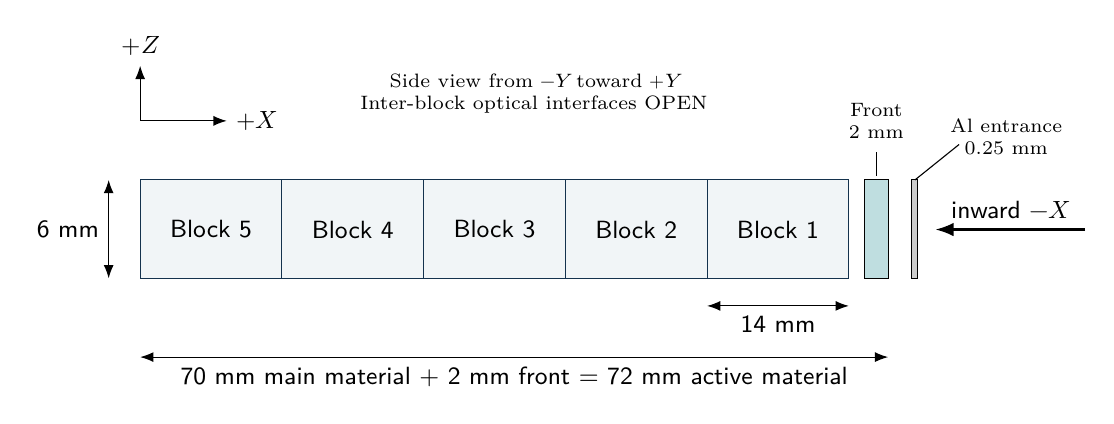
\begin{tikzpicture}[>=Latex,font=\sffamily\small,dim/.style={<->,thin}]
\foreach \x/\n in {0/5,1.8/4,3.6/3,5.4/2,7.2/1}{
\draw[fill=AntaraPale,draw=AntaraNavy] (\x,0) rectangle +(1.8,1.25);
\node at (\x+.9,.62) {Block \n};}
\draw[fill=AntaraTeal!25] (9.2,0) rectangle (9.5,1.25);
\draw[fill=gray!40] (9.8,0) rectangle (9.87,1.25);
\draw[->,thick] (12,.62)--(10.1,.62) node[midway,above]{inward $-X$};
\node[align=center,font=\scriptsize] at (9.35,2) {Front\\2 mm};
\draw (9.35,1.3)--(9.35,1.6);
\node[align=center,font=\scriptsize] at (11,1.8) {Al entrance\\0.25 mm};
\draw (9.84,1.25)--(10.4,1.7);
\draw[dim] (7.2,-.35)--node[below]{14 mm}(9,-.35);
\draw[dim] (0,-1)--node[below]{70 mm main material + 2 mm front = 72 mm active material}(9.5,-1);
\draw[dim] (-.4,0)--node[left]{6 mm}(-.4,1.25);
\draw[->] (0,2)--(1.1,2) node[right]{$+X$};
\draw[->] (0,2)--(0,2.7) node[above]{$+Z$};
\node[align=center,font=\scriptsize] at (5,2.35) {Side view from $-Y$ toward $+Y$\\Inter-block optical interfaces OPEN};
\end{tikzpicture}
\caption{Longitudinal concept, not a packaged CAD drawing. Shown gaps and shield thickness are schematic. Dimension sums count active material only. An optional rear detector would lie beyond Block 5 and is not included.}\label{fig:fpdu-stack-schematic}\label{app:payload-stack}
\end{figure}

\begin{figure}[H]\centering
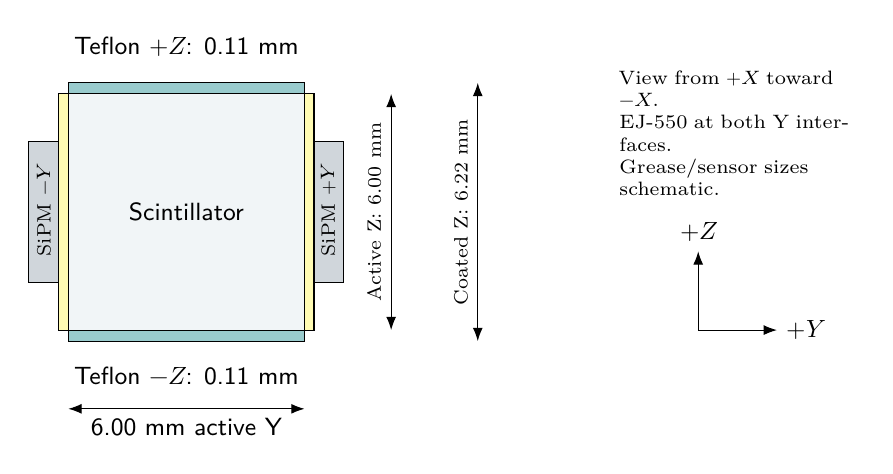
\begin{tikzpicture}[>=Latex,font=\sffamily\small]
\draw[fill=AntaraPale] (0,0) rectangle (3,3);
\draw[fill=AntaraTeal!40] (0,3) rectangle (3,3.14);
\draw[fill=AntaraTeal!40] (0,-.14) rectangle (3,0);
\draw[fill=yellow!30] (-.12,0) rectangle (0,3);
\draw[fill=yellow!30] (3,0) rectangle (3.12,3);
\draw[fill=AntaraNavy!20] (-.5,.6) rectangle (-.12,2.4);
\draw[fill=AntaraNavy!20] (3.12,.6) rectangle (3.5,2.4);
\node[rotate=90,font=\scriptsize] at (-.31,1.5){SiPM $-Y$};
\node[rotate=90,font=\scriptsize] at (3.31,1.5){SiPM $+Y$};
\node at (1.5,1.5){Scintillator};
\node[above] at (1.5,3.35){Teflon $+Z$: 0.11 mm};
\node[below] at (1.5,-.35){Teflon $-Z$: 0.11 mm};
\draw[<->] (4.1,0)--node[midway,sloped,above,font=\scriptsize]{Active Z: 6.00 mm}(4.1,3);
\draw[<->] (5.2,-.14)--node[midway,sloped,above,font=\scriptsize]{Coated Z: 6.22 mm}(5.2,3.14);
\draw[<->] (0,-1)--node[below]{6.00 mm active Y}(3,-1);
\draw[->] (8,0)--(9,0) node[right]{$+Y$};
\draw[->] (8,0)--(8,1) node[above]{$+Z$};
\node[align=left,text width=3cm,font=\scriptsize] at (8.5,2.5){View from $+X$ toward $-X$.\\EJ-550 at both Y interfaces.\\Grease/sensor sizes schematic.};
\end{tikzpicture}
\caption{Main-block cross-section. Optical isolation between successive X faces is undecided. The front scintillator's coating and SiPM attachment face remain open; this cross-section does not prescribe them.}\label{fig:fpdu-cross-section}
\end{figure}

\textbf{OPEN DECISION: optical isolation.} Independently isolated blocks could localize deposition but require defined separators and per-block calibration. Partial longitudinal coupling introduces light sharing and cross-talk that must be measured before using multiplicity or position observables. Common coupling, if physically feasible, would require a calibrated light-sharing model and may reduce deposition localization. None is selected. Surface finish, inter-block material, EJ-550 thickness, photon collection, SiPM saturation and temperature behavior remain unqualified. No controlled current FPDU CAD/ICD was recovered.
\FloatBarrier

\subsubsection{Signal Chain and Timing Trade}\label{app:payload-electronics}\label{app:payload-timing}
\begin{figure}[H]\centering
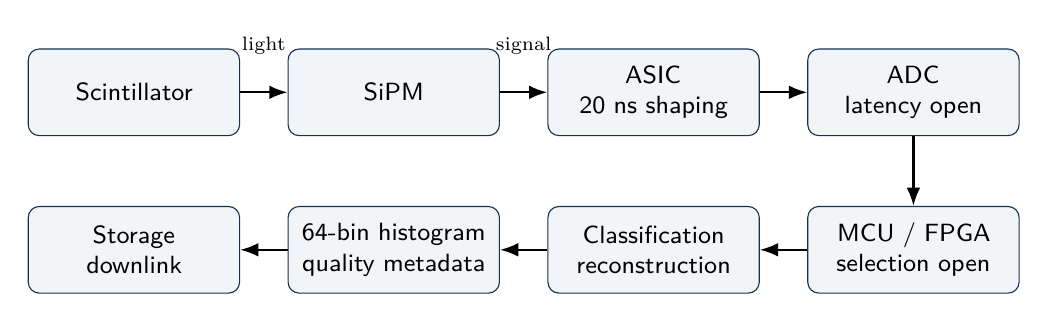
\begin{tikzpicture}[>=Latex,font=\sffamily\small,b/.style={draw=AntaraNavy,fill=AntaraPale,rounded corners,text width=2.45cm,minimum height=1.1cm,align=center},f/.style={->,thick}]
\node[b] (s) at (0,0){Scintillator};
\node[b] (p) at (3.3,0){SiPM};
\node[b] (a) at (6.6,0){ASIC\\20 ns shaping};
\node[b] (d) at (9.9,0){ADC\\latency open};
\node[b] (c) at (9.9,-2){MCU / FPGA\\selection open};
\node[b] (r) at (6.6,-2){Classification\\reconstruction};
\node[b] (h) at (3.3,-2){64-bin histogram\\quality metadata};
\node[b] (o) at (0,-2){Storage\\downlink};
\draw[f] (s)--node[above=10pt,font=\scriptsize]{light}(p);
\draw[f] (p)--node[above=10pt,font=\scriptsize]{signal}(a);
\draw[f] (a)--(d);\draw[f] (d)--(c);\draw[f] (c)--(r);\draw[f] (r)--(h);\draw[f] (h)--(o);
\end{tikzpicture}
\caption{Candidate signal and science-data flow. EJ-550 provides the optical interface. Eleven SiPMs do not specify eleven ADCs. Fast coincidence may occur in analog/ASIC logic while downstream processing is buffered; this architecture remains to be selected.}\label{fig:fpdu-signal-chain}
\end{figure}

\begin{table}[H]\centering\small
\caption{Separate timing references and missing qualification inputs}\label{tab:fpdu-timing}
\begin{tabularx}{\linewidth}{@{}p{4.2cm}p{2.4cm}X@{}}\toprule
Quantity & Planning input & Interpretation\\\midrule
ASIC shaping time & 20 ns & Pulse-shaping parameter, not coincidence or dead time\\
Coincidence target & 200 ns & Nominal acceptance-window reference\\
Initial timing allowance & $\geq250$ ns & Margin-inclusive window reference\\
Preferred allowance & $\sim300$ ns & Comfortable window reference; accidental-coincidence trade required\\
Post-shaping delay & 20 ns stated & Meaning unresolved; not assigned as ADC conversion latency\\
ADC conversion / processing & Unknown / unknown & Datasheets, pipeline and worst-case execution measurements required\\
Qualified detector dead time & Unknown & Shared/per-channel topology and loss model unresolved\\
Timestamp precision / jitter & Unknown & Channel skew and discriminator/capture measurements required\\
Maximum trigger throughput & Unknown & All-particle acceptance, burst and queue tests required\\\bottomrule
\end{tabularx}\end{table}

The 200/250/300~ns values are coincidence-window planning references, as clarified by the team. They are not processor execution deadlines. Widening a window changes accidental coincidences; it does not prove engineering margin. The two stated 20~ns values must not simply be summed into an end-to-end latency. No dead time is assigned from any of these values.

MCU is preferred only if the complete acquisition architecture demonstrates adequate timestamp precision, coincidence handling, ADC bandwidth, buffering, processing throughput and power. Compare ASIC/discriminator coincidence with MCU processing, timer/capture-assisted MCU, FPGA, and hybrid FPGA/MCU implementations. For a stated mean arrival rate $\lambda$ and service time $s$, $\lambda s<1$ is a queue-stability prerequisite, not proof of low event loss. Finite buffers and burst arrivals need explicit tests. Coincidence, ADC acquisition, service time, event loss and detector livetime remain separate quantities.
\FloatBarrier

\subsubsection{Radiation Inputs and Conditional Rate Estimates}\label{app:payload-data}
The supplied AP9/AE9 maps are integral omnidirectional fluxes at MJD 61041 (1 January 2026), altitude 600~km. They are team-approved preliminary references for 2029 mission planning, not regenerated 2029 environment outputs. The rate conversion assumes isotropy and $G=1$~cm$^2$~sr with unit efficiency: $R=F_{\rm omni}G/(4\pi)$. It uses log--log interpolation at 5.5~MeV for protons and 0.35~MeV for electrons. The script contains no aluminium transport, actual telescope acceptance, electron rejection, optical response or dead-time model.

\begin{table}[H]\centering\small
\caption{Reproduced MODEL PREDICTIONS: idealized incident-rate proxy maxima (Hz)}\label{tab:fpdu-rates}
\begin{tabularx}{\linewidth}{@{}lrrX@{}}\toprule
Map & Proton & Electron & Interpretation\\\midrule
Mean & 358.920 & 67\,779.655 & Nominal preliminary environment\\
99th percentile & 975.659 & 503\,419.743 & Conservative study scenario, not a hard upper bound\\\bottomrule
\end{tabularx}\end{table}
The species maxima need not occur at the same cell. Maximum same-cell summed proxies are 68\,055.635~Hz (mean) and 504\,245.064~Hz (99th-percentile maps); the latter is not a joint 99th-percentile trigger bound. Values are independently reproduced from \path{data/raw/payload_count_rate_2026/} in the count-rate validation report. Flux-times-area proxy columns must not be confused with the columns divided by $4\pi$.

\textbf{PRELIMINARY ESTIMATE, superseded rounded reference:} approximately 400~Hz assumed protons only, 250~$\mu$m (0.25~mm) aluminium shielding, geometric factor 1~cm$^2$~sr and 100\% detection efficiency. Its original generating calculation remains unidentified. The supplied per-cell rates take priority; they do not implement the stated aluminium shielding. No constant rate or electronics ceiling is imposed.

The proton source grid ends at an integral threshold of 20~MeV; its above-threshold quantities are not truncated differential bins. It cannot supply a calibrated 5--100~MeV spectrum or an integral subtraction at 100~MeV. Electrons may consume front-end resources before downstream rejection. A credible maximum actual trigger rate requires geometry, transport, thresholds, mixed species and burst evidence and is not established here.

\subsubsection{Reconstruction, Histogram and Telemetry Contract}\label{app:payload-coincidence}\label{app:payload-readout}
The front scintillator is intended to respond in the proposed 5.5--15~MeV incident range and provide deposition, path-length-corrected d$E$/d$x$, and classification/coincidence observables. These functions are not calibrated incident-energy measurements. Response-matrix lookup/unfolding and a trained reconstruction model remain candidates. Evaluation must use detector observables, keeping truth energy only as the reference target. The old five-layer stopping response and silicon-based coincidence do not apply.

\begin{table}[H]\centering\small
\caption{Science Record v3: 292-byte uncompressed reference, excluding radio framing}\label{tab:fpdu-telemetry}
\begin{tabularx}{\linewidth}{@{}p{3.6cm}rX@{}}\toprule
Field & Bytes & Reference encoding\\\midrule
Entry / exit timestamps & 16 & Two uint64 microsecond POSIX UTC values since 1970-01-01; half-open interval\\
Latitude / longitude & 8 & Two signed int32, degrees $\times10^7$; midpoint WGS84 geodetic position\\
Altitude & 4 & Signed int32 millimetres above WGS84 ellipsoid\\
64 histogram bins & 256 & uint32 integer counts, provisional 5--100~MeV reporting edges\\
Sequence & 4 & uint32; reboot/wrap epoch in session manifest\\
Combined status & 2 & uint16 mode and six subsystem-health pairs\\
CRC16 & 2 & CRC-16/IBM-3740 over preceding 290 bytes\\\midrule
Total & 292 & Little endian, no padding; no radio overhead included\\\bottomrule
\end{tabularx}\end{table}
The reference definition is \path{config/science/science_record_v3.json}. Version, bin-edge ID \texttt{FPDU-log64-5-100-v1}, calibration/response/configuration identity and time correlation are mandatory linked session metadata, not hidden extra bytes in the record. Actual livetime, losses, background and quality details require linked interval metadata whose size remains unbudgeted. The 64 bins are not 64 independently calibrated channels. Fractional modeled expectations are not valid uint32 measured counts.

CRC polynomial is 0x1021, initial value 0xFFFF, nonreflected, final XOR zero; CRC bytes are little endian. The reference check for ``123456789'' is 0x29B1. UTC leap seconds are not representable in POSIX time; split/flag affected acquisitions and retain clock correlation. Encoding resolution is not clock or navigation accuracy. No final radio packet size or throughput qualification is implied.

\begin{table}[H]\centering\small
\caption{Combined 16-bit mode and health codebook}\label{tab:status-v3}
\begin{tabularx}{\linewidth}{@{}>{\raggedright\arraybackslash}p{3.6cm}X@{}}\toprule
Bits & Meaning\\\midrule
0--3 & 0 Cold/Dark; 1 Detumble; 2 Sun Pointing; 3 Detection; 4 Relay; 5 Slewing; 6 Safe; 7--14 reserved; 15 unknown\\
4--5 / 6--7 / 8--9 & OBC / EPS / ADCS health\\
10--11 / 12--13 / 14--15 & COMMS / payload / other-thermal health\\
Each health pair & 00 nominal; 01 degraded; 10 fault; 11 unknown\\\bottomrule
\end{tabularx}\end{table}
These new serialization codes map the actual FSM names, not pre-existing numeric telemetry values. Unknown health must not default to nominal. Detailed diagnostics are separate; this marker cannot replace calibrated exposure or background information.

\paragraph{Reading validity and accumulation.}
Prefer three readings per eligible geographic cell visit, with two or one when available timing permits; no valid exposure means no record. No arbitrary minimum duration or count threshold is imposed. Each reading has its own positive, nonoverlapping interval, geographic attribution and valid acquisition state. Split at cell/mode boundaries and shutdown; do not bridge off periods. Valid zero-count records are retained. Realizable boundaries depend on timer resolution, readout latency and uninterrupted counter handoff, all still unqualified. A short interval can be a valid record without achieving a mission precision target.

For an ideal zero-background Poisson diagnostic, accumulated fractional counting uncertainty is $1/\sqrt{\sum_i N_i}$, not an average of individual fractional errors. Background, livetime and reconstruction uncertainty remain necessary. Zero-count exposures contribute to inference and must not be discarded. Splitting a visit preserves total exposure and counts and does not create independent orbital passages. Approved MMSC/MSC/EMSC requirements are unchanged. The offline reference partitions closed acquisition segments; the flight scheduler and event-buffer/counter-bank design require PDR verification.

For directional differential flux $\Phi_s$ in cm$^{-2}$~s$^{-1}$~sr$^{-1}$~MeV$^{-1}$ and effective area $A_{j,s}$ in cm$^2$, the response contract is
\begin{equation}
N_j=\int\ell(t)\sum_s\int\!\int A_{j,s}(E,\Omega,t)\Phi_s(E,\Omega,t)\,dE\,d\Omega\,dt.
\end{equation}
A geometric factor already includes the angular integral. Shared-trigger livetime, energy migration, background subtraction and calibration uncertainty require a qualified model. Geometric coverage or synthetic counting precision alone cannot establish MMSC, MSC or EMSC.

\subsubsection{Geometric-Factor Requirement from Cell Counts}\label{app:required-g}
\textbf{MODEL PREDICTION; arithmetic independently reproduced.}
The supplied geometric-factor study asks how much ideal proton acceptance is needed to reach a counting-only precision target in each cell. It uses 7940 unique 0.5$^\circ$ polygon-overlap cells, integral-spectrum differences and supplied cell dwell times of 98--294~s. The dwell file matches an archive labelled ``18-Month Simulation'', but the executed configuration and duration are missing. Nearby source defaults to three days and cannot explain the accumulated table. No mission-duration scaling is applied. The radiation table is AP9-labelled; its actual mean/percentile setting, epoch and 65-threshold source run remain unverified. It is distinct from the verified 2026 AP9/AE9 maps above.

Under isotropy, unit efficiency and a scalar geometric factor,
\begin{equation}
R_{u,c,b}=\frac{F_c(>E_{b,\mathrm{lo}})-F_c(>E_{b,\mathrm{hi}})}{4\pi},\qquad
N_{c,b}=R_{u,c,b}G\epsilon T_c,\qquad
G_{\mathrm{req},c,b}=\frac{1}{\sigma^2R_{u,c,b}\epsilon T_c}.
\end{equation}
Here $F$ is omnidirectional integral flux in cm$^{-2}$~s$^{-1}$, $R_u$ is rate per unit $G$ in s$^{-1}$/(cm$^2$~sr), $T$ is supplied dwell in seconds, and $G$ is in cm$^2$~sr. No extra energy width or angular integral is applied. The expected-count targets for $\sigma=10,15,25,50\%$ are 100, 44.44, 16 and 4; these are not total reconstructed-flux uncertainties or guarantees on realized counts.

\begin{table}[H]\centering\small
\caption{Reproduced required $G_{95}$ for each separately selected cell population; $\epsilon=1$, cutoff 5.4~MeV, supplied dwell. All $G$ values are cm$^2$~sr.}\label{tab:required-g}
\begin{tabular}{@{}lrrrrr@{}}\toprule
Band (MeV) & Cells & 10\% & 15\% & 25\% & 50\%\\\midrule
5.4--10 & 7596 & 0.364535 & 0.162016 & 0.058326 & 0.014581\\
10--20 & 7177 & 0.413303 & 0.183690 & 0.066129 & 0.016532\\
20--40 & 7052 & 0.500042 & 0.222241 & 0.080007 & 0.020002\\
40--100 & 7144 & 0.360776 & 0.160345 & 0.057724 & 0.014431\\\bottomrule
\end{tabular}\end{table}

Each band selects cells with rate at least 1\% of its own peak and takes the linearly interpolated 95th percentile of their required $G$. This resembles one ingredient of EM-M-02, but does not establish its mission-peak eligibility definition or joint channel coverage. At the hypothetical $G=0.3$~cm$^2$~sr, the 10\% counting-target coverages are 93.55, 92.25, 89.66 and 93.25\% of these respective populations. All four meet the 25\% expected-count target in their selected cells. These are not mission-success percentages.

\begin{figure}[H]\centering
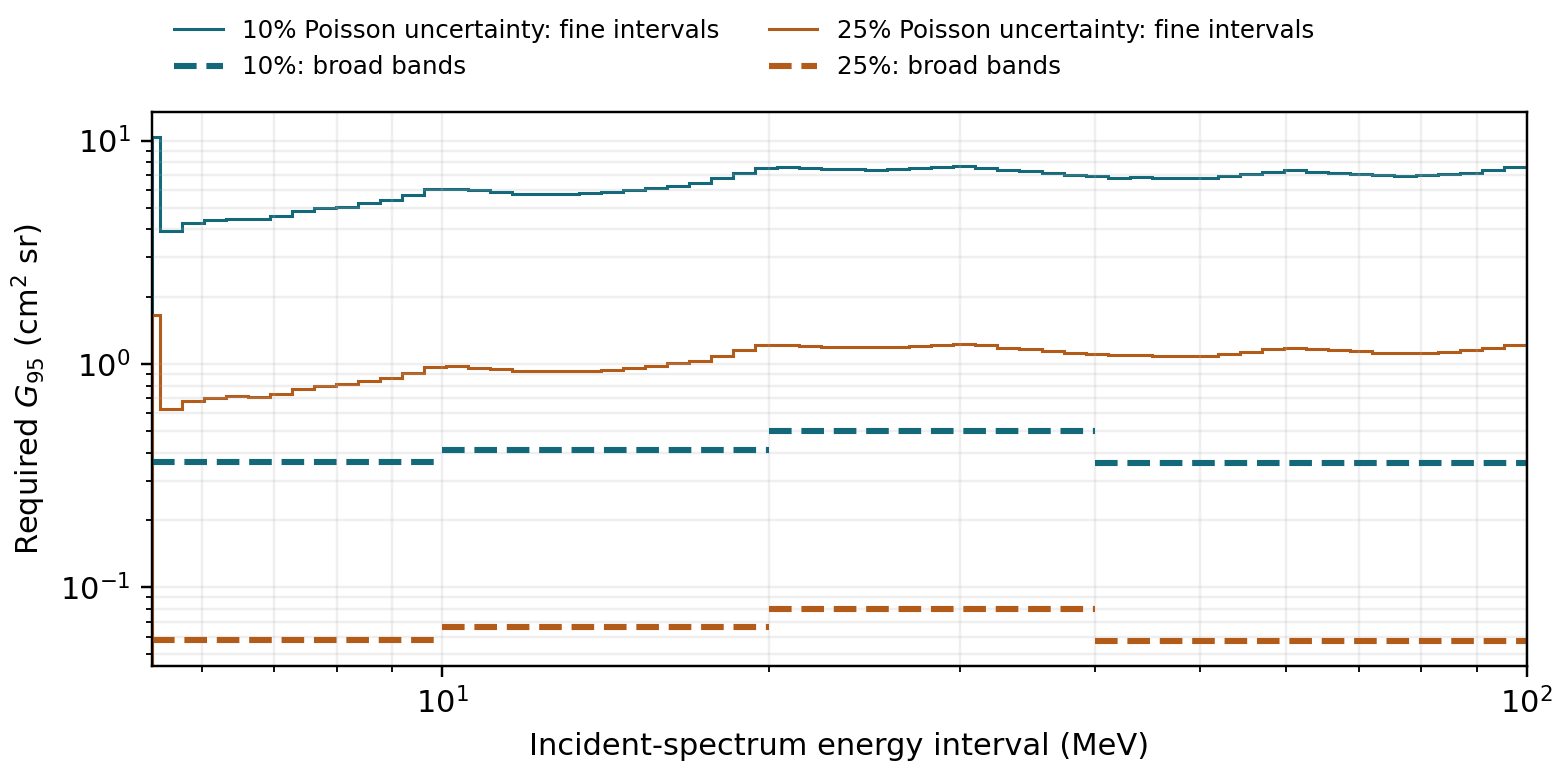
\includegraphics[width=\linewidth]{media/geometric_factor_requirements.png}
\caption{Independent reproduction of the required-$G$ study. Fine intervals require more acceptance for the same counting precision than broad bands; each interval has its own eligible-cell population. This is a count requirement, not an achievable or measured FPDU response.}\label{fig:required-g-binning}
\end{figure}
The input has 65 thresholds over 5--100~MeV, giving 64 intervals. The 5.4~MeV cutoff removes the first and truncates the second, leaving 63 intervals. Their 10\% $G_{95}$ values span 3.9284--10.3301~cm$^2$~sr, compared with 0.3608--0.5000 for the broad bands. Neither is evidence for 64 resolved channels. The provisional 64-bin telemetry retains its separate 5--100~MeV definition; merging reporting bins does not establish the required energy resolution.

\paragraph{Required versus achievable acceptance.}
An ideal unrestricted one-sided 6~mm square aperture has $G=\pi A=1.13097$~cm$^2$~sr. Two equal aligned planes separated by 2~mm, 4.8~mm or 72~mm give approximately 0.61907, 0.29743 or 0.0024885~cm$^2$~sr, respectively. These are hypothetical straight-track acceptance conditions: no collimator, material or all-block coincidence rule is selected. Crossing both ends of a gap-free aligned 72~mm assembly implies crossing every block, but early-stopping or side-exiting particles need different acceptance logic. The supplied optional model assigns on-axis stopping depths using illustrative EJ-200 and a simplified CSDA approximation; it omits angular transport, scattering, straggling and qualified triggers. It cannot establish the actual energy-dependent effective $G$. Its coarse quadrature also overestimates the artificial 0.2~mm separation case by about 3.6\%.

\paragraph{Cutoff, exposure and PDR conditions.}
The default 5.4~MeV cutoff is a hard study assumption, not aluminium transport. The optional source approximation instead derives about 5.95~MeV for 250~$\mu$m Al; neither value is a validated transmission threshold. Changing only the counting cutoff to 5.5~MeV increases first-band $G_{95}(10\%)$ to 0.380454~cm$^2$~sr (4.37\%), with 7588 selected cells. The committed 5--100~MeV requirement is unchanged. Required $G$ scales inversely with effective efficiency and verified exposure; no duration extrapolation is justified by the current manifest gap. Background subtraction, livetime, reconstruction covariance, independent passages, temporal maps and stored/downlinked records must be validated before tier acceptance. Source hashes, reproduced tables and tests are indexed in \path{docs/audit/GEOMETRIC_FACTOR_NUMERICAL_VALIDATION.md}.

\subsubsection{Conditions for PDR Closure}\label{app:payload-transport}\label{app:payload-calibration}
\begin{table}[H]\centering\small
\caption{Remaining verification conditions}\label{tab:fpdu-response-matrix}
\begin{tabularx}{\linewidth}{@{}p{3.4cm}X@{}}\toprule
Interface & Required closure evidence\\\midrule
Mechanical / optical & Controlled CAD/ICD, material, front treatment, gaps, optical isolation, grease and SiPM placement; measured cross-talk and collection maps\\
Transport / acceptance & Current six-scintillator geometry, entrance Al, proton 5--100~MeV and electron/species/angular scans; validate effective geometric factor\\
Electronics & Selected channels/components, post-shaping interpretation, timing/jitter, queue/burst tests, measured dead time and loss counters\\
Reconstruction & Independent calibration and test data, stopping/penetrating response, mixed-species confusion matrix and injected-spectrum closure\\
Mission coupling & Science-enabled exposure, qualified channels/background, independent-observation contract and stored/downlinked records before tier acceptance\\\bottomrule
\end{tabularx}\end{table}

\clearpage
\subsection{Simulation Configuration and Provenance}
\label{app:sim-provenance}

This appendix records the simulation code used to support the ANTARA mission concept. The simulation scripts are organised by study under \texttt{src/simulations/}. The integrated science simulation uses a common configuration defined in \path{src/simulations/helper/antara_models.py}; the standalone orbit, power, pointing, detumble, CONOPS and thermal studies have their own study-specific configurations. Their results must not be treated as outputs of one identical spacecraft model unless the input parameters have been checked.

\subsubsection{Simulation Inventory}
\label{app:sim-inventory}
\begin{longtable}{p{0.20\linewidth}p{0.43\linewidth}p{0.28\linewidth}}
\caption{Simulation source files and principal applications.}\label{tab:simulation-source-inventory}\\
\toprule
Study & Python entrypoint(s) & Intended evidence \\
\midrule
\endfirsthead
\toprule Study & Python entrypoint(s) & Intended evidence \\
\midrule
\endhead
Integrated science and DITL & \texttt{ditl/ANTARA\_Science\_Sim.py}; \texttt{ditl/scenarios.py}; \texttt{ditl/compare\_scenarios.py} & Mission modes, power, attitude, SAA science opportunities and ground contact \\
Orbital decay & \texttt{orbit/ANTARA\_drag\_finalconfig.py}; \texttt{orbit/ANTARA\_drag\_study.py} & Orbital decay and lifetime studies \\
Power & \texttt{power/ANTARA\_MCR.py}; \texttt{power/ANTARA\_avg.py}; \texttt{power/ANTARA\_FINAL\_POWERGEN.py}; \texttt{power/TradeCase.py} & Power-generation and battery trade studies \\
Pointing & \texttt{pointing/ANTARA\_pointing\_budget.py} & Ground-station pointing geometry \\
Detumble & \texttt{detumble/leop\_detumble\_mc.py}; \texttt{detumble/analyze\_detumble\_mc.py} & Initial-rate reduction and Monte Carlo statistics \\
CONOPS & \texttt{conops/ANTARA\_conops.py} & SAA and station encounter analysis \\
Thermal & \texttt{thermal/ThermalSimulator.py} & Lumped-parameter temperature studies \\
Shared support & \texttt{helper/antara\_models.py}; \texttt{helper/fsm\_spec.py}; \texttt{helper/telemetry\_metrics.py}; other \texttt{helper/} modules & Configuration, attitude models, FSM rules and telemetry processing \\
Historical & \texttt{legacy/ANTARA\_Master.py} & Superseded simulation; not a current baseline \\
\bottomrule
\end{longtable}

\subsubsection{Integrated Simulation Baseline}
\label{app:integrated-sim-baseline}
The values in Table~\ref{tab:science-model-defaults} are the defaults in \texttt{MissionConfig} supplied with the reviewed source archive. These are simulation inputs, not final hardware qualifications or independent performance measurements. A command-line override or a run-specific configuration can change them.

\begin{longtable}{p{0.47\linewidth}p{0.29\linewidth}p{0.16\linewidth}}
\caption{Selected integrated simulation configuration defaults.}\label{tab:science-model-defaults}\\
\toprule Parameter & Code-defined value & Unit \\
\midrule
\endfirsthead
\toprule Parameter & Code-defined value & Unit \\
\midrule
\endhead
Initial orbital altitude & 600 & km \\
Inclination & 97.6 & degrees \\
Eccentricity & 0.001 & --- \\
RAAN & 15 & degrees \\
Initial spacecraft mass & 3.0 & kg \\
Drag coefficient & 2.2 & --- \\
SRP coefficient & 1.8 & --- \\
Simulation start date & 1 March 2000 & UTC calendar date \\
Nominal fine time step & 2 & s \\
Coarse time step & 20 & s \\
Battery planning capacity & 25 & Wh \\
Initial stored battery energy & 18 & Wh \\
EPS charge efficiency & 0.88 & --- \\
Solar temperature derating & 0.88 & --- \\
Maximum solar generation parameter & 22 & W \\
OBC load parameter & 0.8 & W \\
EPS load parameter & 1.2 & W \\
Payload load parameter & 10 & W \\
Radio transmit load parameter & 12 & W \\
ADCS idle and slew loads & 0.8 / 4.5 & W \\
Radio downlink rate & 0.0192 & Mbit/s \\
Primary ground-station location & $15^\circ$ N, $74^\circ$ E & coordinates \\
Ground-station altitude & 70 & m \\
Ground-station elevation mask & 15 & degrees \\
Random seed & 42 & --- \\
\bottomrule
\end{longtable}

The integrated model also defines power thresholds for entering and exiting low-power conditions, attitude-pointing limits, detection and relay minimum durations, a maximum wheel-saturation hold, and fault/recovery debounce settings. The exact configuration used for a reported run must be retained with that run, rather than inferred only from current defaults.

\subsubsection{Integrated DITL Scenarios}
\label{app:ditl-scenarios}
The three standard presets are defined in \texttt{ditl/scenarios.py} and shown in Table~\ref{tab:science-scenario-presets}. The two 24-hour cases separate the startup sequence from nominal operations; the one-year preset includes startup.

\begin{table}[htbp]
\centering
\caption{Integrated Science simulator presets.}
\label{tab:science-scenario-presets}
\begin{tabularx}{\linewidth}{l r X}
\toprule
Preset & Duration & Starting condition \\
\midrule
\texttt{leop\_24h} & 24 h & Includes cold-start and detumble sequencing \\
\texttt{no\_leop\_24h} & 24 h & Skips LEOP and starts in Sun Pointing \\
\texttt{leop\_1yr} & 8,760 h & Includes LEOP; uses multirate integration with a configured 20 s coarse step \\
\bottomrule
\end{tabularx}
\end{table}

Configuration precedence in the source is explicit command-line options, followed by scenario preset, followed by the global defaults. In particular, the RAAN and battery capacity are configuration fields and are not exposed as direct \texttt{--raan-deg} or \texttt{--battery-wh} command-line options in the documented Science entrypoint.

\subsubsection{Numerical and Physics Models}
\label{app:physics-assumptions}
The integrated simulator uses Orekit numerical orbit propagation and includes gravitational perturbations, an atmospheric drag model and solar radiation pressure. The source imports the Holmes--Featherstone gravity-field model and the DTM2000 and NRLMSISE-00 atmospheric models. The model and options active in a particular run must be established from the saved configuration and executed code path.

The integrated model uses scalar-first quaternions, $[w,x,y,z]$, for body-to-inertial attitude transformations. The spacecraft body axes are defined with $+X$ along the payload boresight, $+Y$ toward the relay antenna and $+Z$ along the fixed solar-panel face. The simulation includes finite slews and pointing-settlement checks; an attitude command does not produce an instantaneous orientation change.

The magnetic-field implementation supports the configured dipole option and an IGRF backend through \texttt{ppigrf}. If the optional IGRF package is unavailable, the documented IGRF path warns and falls back to a centred dipole. This fallback is not equivalent to an IGRF-based result and must be recorded when used.

The proton environment model applies SAA spatial variation, magnetic pitch-angle dependence, east--west asymmetry, storm scaling and detector response to a configured baseline spectrum. Although a legacy interface and some telemetry keys use the name \texttt{ap9}, the present source does \emph{not} execute a live AP9 calculation. Consequently, simulator flux values must not be represented as independently generated AP9 predictions or validated in-orbit measurements. The simulator's detector counts are modeled expected counts, rather than a calibrated hardware measurement campaign.

\subsubsection{Time Accounting and Data Outputs}
\label{app:data-reproduction}
The Science simulator writes scenario-tagged CSV files under \texttt{results/science/}, including telemetry, SAA passes, ground-station contacts, mode transitions, slew events, detumble events, rejected transitions and proton passes. Figures are written under \texttt{figures/science/} when plot generation is enabled.

Newer source telemetry distinguishes the row observation time, \texttt{time\_sec}, from the integrated interval end, \texttt{state\_time\_sec}. \texttt{interval\_duration\_sec} records the elapsed integration interval. Those interval columns are absent from the corrected exports. This audit uses successive recorded timestamps, assigns no duration after the endpoint, and retains timing-semantic uncertainty. In the newer source, the final terminal snapshot has zero duration. Time-averaged quantities and mode occupancy must therefore be weighted by the interval durations rather than the number of CSV rows. Plot sampling is for display only; extrema and scientific statistics should be calculated from complete telemetry and validated summary outputs.

The simulator supports trusted, versioned checkpoints and resumable execution. Checkpoints and their linked science-event archives must be retained together. A resume record does not by itself establish that the entire intended scenario completed correctly.

\subsubsection{Supporting Study Differences}
\label{app:study-differences}
The standalone scripts should be treated as supporting studies rather than interchangeable implementations of the integrated Science scenario. In particular:
\begin{itemize}
\item The standalone pointing-budget study uses its own nadir-pointing and antenna-boresight assumptions; these must be compared with the integrated $+Y$ relay antenna geometry before a result is used as the spacecraft relay pointing budget.
\item Standalone solar-power and battery studies contain their own panel and operating assumptions, which must be reconciled with the integrated Science configuration.
\item Detumble Monte Carlo trials are useful for testing the controller over initial conditions, but do not automatically demonstrate integrated EPS, payload and ground-station operation.
\item The thermal model is a separate lumped-parameter study, not a temperature field directly solved within every Science simulator step.
\item The historical \texttt{ANTARA\_Master.py} is superseded and should not be used as the current simulation baseline.
\end{itemize}

\subsubsection{Verification Status and Known Limits}
\label{app:model-limits}
The supplied repository's \texttt{docs/CURRENT\_STATUS.md} records a 414-test software regression run during Phase 3B and matching one-hour Science baseline outputs. These are repository-reported verification results; they have not been independently reproduced in preparing this appendix. The same record states that a 60-hour annual-preset run does not establish completion or validation of the full one-year scenario. It also identifies the absence of live AP9 calculation and the superseded status of the Master implementation.

For each figure or numerical conclusion adopted in the MCR, retain the following alongside the output: source revision or commit, scenario name, complete run configuration, RNG seed where applicable, simulator start date, run duration and completion status, numerical step controls, output path, and any modifications to the baseline model. Without these details, a plotted quantity cannot be reliably associated with a particular spacecraft design configuration.

\subsubsection{Simulation Evidence Record}
\label{app:evidence-record}
The following records distinguish approved planning inputs from verified generating epochs. Full claims and hashes are indexed in the audit reconciliation and count-rate ingestion reports.
\begin{table}[H]\centering\small
\caption{Current evidence identities and limits}\label{tab:evidence-record-template}
\begin{tabularx}{\linewidth}{@{}p{3cm}p{4cm}X@{}}\toprule
Evidence & Identity & Acceptance limit\\\midrule
Mission baseline & \texttt{ANTARA-2029-v1}; 2029-01-01 & Approved configuration, not completed run\\
Radiation rate maps & MJD 61041; 600 km; AP9/AE9 mean and 99th percentile & Reproduced arithmetic; 2026 source accepted for preliminary 2029 planning\\
RAAN study & Seven cases, two runs each; supplied CSVs & Team-accepted 2029 reference; generating epoch not independently verified\\
Historical DITL & March 2000 source run & Historical operational example, not current payload qualification\\
Corrected Science exports & Two 24 h and one 365-day timestamp spans; March 2000 & Runtime source/configuration and mode semantics unresolved\\
Required-$G$ study & 7940 cells; 65 integral thresholds; supplied dwell & Tables reproduced; source epoch, percentile and exposure duration unverified\\
Current FPDU & Approved-v2 configuration & Mechanical inputs and logical interfaces only; no qualified response\\\bottomrule
\end{tabularx}\end{table}

\paragraph{Payload and software reconciliation.}
The current configuration is not consumed by the legacy DITL/Geant4 response. Eleven SiPMs, removed silicon, open optics and unknown dead time require geometry-matched validation. Coincidence references are 200/250/300~ns; shaping is 20~ns. Historical outputs remain unchanged. Bounded tests validate accounting only. Tested source fixes are delivered as an unapplied patch because the authoritative simulator is outside the writable workspace.

\subsubsection{New Operational, Thermal and Detumble Evidence}\label{app:new-run-identities}
Corrected Science authority is controlled by \path{evidence/science-ditl/run_registry.json}; prior Science manifests are superseded. Independent study manifests remain under \path{evidence/science-ditl/manifests/}, \path{evidence/thermal/manifests/} and \path{evidence/detumble/manifests/}. Current external source hashes are candidate references only; no generating commit or runtime manifest was supplied. Command-line duration overrides cannot be recovered from preset names.
\begin{table}[H]\centering\small
\caption{Observed evidence completeness; no expensive simulation rerun}\label{tab:new-run-completeness}
\begin{tabularx}{\linewidth}{@{}p{3cm}p{3.1cm}X@{}}\toprule
Evidence & Observed span & Acceptance boundary\\\midrule
Corrected LEOP / No-LEOP & 7696 / 6553 rows; 0--86400 s & Complete timestamp spans; runtime configuration unknown\\
Corrected annual telemetry & 1434872 rows; 0--31536000 s & Complete365-day timestamp span; interval semantics conditional\\
Corrected annual events & 2000-03-01 epoch & Contact/data totals reconcile; mode/slew definitions require closure\\
Thermal & 43\,201 labels; 0--24~h; 2~s & One history; no separate HOT/COLD cases; initial-state timing unresolved\\
Detumble & 50\,000 summary rows & Historical inputs incompatible with current source; censor times/seed absent\\\bottomrule
\end{tabularx}\end{table}
Current candidate orbit and thermal integrators are DP853 and RK4 respectively, but defaults cannot establish the producing solver settings. The thermal heat schedule is independent of DITL. Passing local accounting tests establishes parsing, interval weighting and summary arithmetic only; it does not validate current hardware response or a common 2029 run.

\paragraph{Science-record and communications revision.}
Science Record v3 and the full 19.2~kbps capacity analysis are new MCR reference interfaces, not outputs of the historical simulator. Source hashes and exact per-contact/tier calculations are under \path{data/derived/ditl_correction_2026-11-09/}; the generating scripts read originals without changing them. The grid-study horizon remains unknown, annual contacts retain their 2000 epoch, and corrected telemetry spans365days; the old partial artifact is superseded. The 292-byte reference supersedes older unencoded record-size assumptions without modifying detector physics, scientific thresholds or original transfers.

\clearpage

\subsection{Thermal and Structural Supporting Analysis}\label{app:thermal-structural}
This appendix describes the thermal model implemented in \path{src/simulations/thermal/ThermalSimulator.py} and the structural information available in the MCR. The thermal results are model predictions; no spacecraft-level thermal-vacuum or mechanical qualification is claimed.
\subsubsection{Thermal Model and Spacecraft Geometry}\label{app:thermal-model}
The simulator represents the spacecraft with seven lumped-capacitance nodes: the six external faces and an internal bus. The geometric model uses a $10\times10\times34$~cm 3U body with the long axis along $X$. Each end face has area $0.010$~m$^2$ and each long face has area $0.034$~m$^2$. Each node carries mass, specific heat, solar absorptivity, infrared emissivity and thermal conductance to the internal bus. Neighboring external faces are also coupled through a specified conductance. These values form a preliminary thermal representation, not measured properties of the final assembly.
\begin{table}[htbp]\centering\caption{Selected thermal simulation inputs (\texttt{ThermalMissionConfig} defaults).}\label{tab:thermal-config}\begin{tabularx}{\linewidth}{Xl}\toprule Input & Code setting\\\midrule
Initial orbit altitude / inclination & 600~km / $97.6^\circ$\\
RAAN and eccentricity & $15^\circ$ / 0.001\\
Spacecraft model mass & 3.0~kg\\
Simulation duration / nominal time step & 24~h / 2~s\\
Thermal substeps per simulation step & 10\\
Initial temperature & 293.15~K\\
Internal bus lumped mass / specific heat & 1.8~kg / 800~J\,kg$^{-1}$\,K$^{-1}$\\
Face-to-face thermal conductance & 0.05~W\,K$^{-1}$\\
Solar constant / deep-space temperature & 1361~W\,m$^{-2}$ / 2.7~K\\
Applied temperature margin parameter & $10^\circ$C\\\bottomrule\end{tabularx}\end{table}
\subsubsection{Thermal Balance and Numerical Method}\label{app:thermal-equations}
For each node $i$, the model integrates a lumped heat balance of the form
\begin{equation}\label{eq:thermal-balance}
C_i\frac{\mathrm{d}T_i}{\mathrm{d}t}=Q_{\mathrm{solar},i}+Q_{\mathrm{albedo},i}+Q_{\mathrm{EarthIR},i}+Q_{\mathrm{internal},i}-Q_{\mathrm{radiated},i}+\sum_j G_{ij}(T_j-T_i),\qquad C_i=m_ic_i.
\end{equation}
The code calculates incident solar radiation, Earth albedo and infrared heating, thermal emission, internal dissipation and conduction. Solar-cell electrical conversion is included in the face heat balance. The orbit is propagated with Orekit numerical integration; the thermal equations use fourth-order Runge--Kutta integration with configurable thermal substeps. Earth albedo and infrared terms may vary with latitude in the implemented model.
\subsubsection{Nominal, Hot and Cold Cases}\label{app:thermal-cases}
The source defines \texttt{NOMINAL}, \texttt{HOT} and \texttt{COLD} bounding-case configurations. Nominal retains the base configuration. The HOT case places the model near perihelion, increases the end-of-life optical assumption and adds 0.5~W of bus dissipation. The COLD case uses an aphelion epoch, a lower optical assumption and 0.5~W less bus dissipation; relay and detection loads are disabled for that case. These are deliberately selected model cases, not measured flight extremes. The simulation can also use LVLH or prescribed tumbling attitude.
The default internal heat schedule is independent of the Science DITL flight software: it includes a 1.5~W baseline bus, 0.4~W charging term, 0.8~W eclipse-heater term, a 3.0~W relay-pass increment and a 1.2~W detection-window increment with configured durations. Consequently, thermal case temperatures should not be described as arising from the exact commanded state history of \texttt{ANTARA\_Science\_Sim.py}.
\subsubsection{Temperature Outputs and Required Comparison}\label{app:thermal-output}
The supplied history contains 43\,201 unique time labels from 0 to 24~h. Kelvin/Celsius pairs and all summary extrema/timestamps reproduce independently. Table~\ref{tab:thermal-observed} reports the recorded envelope. Time-weighted means use trapezoidal integration over labels, without adding an interval beyond 24~h. Nonuniform first logged temperatures differ from the candidate 293.15~K initialization; the exact generating source and possible state-label offset require reconciliation.
\begin{table}[H]\centering\small
\caption{Single-history node statistics; degrees Celsius. No component compliance margin is established.}\label{tab:thermal-observed}
\begin{tabular}{@{}lrrr@{}}\toprule Node & Minimum & Maximum & Time-weighted mean\\\midrule
+X & -20.775 & 19.914 & -8.907\\
-X & -17.220 & 26.911 & -5.480\\
+Y & -15.865 & 19.951 & -9.507\\
-Y & -25.958 & 31.239 & -7.625\\
+Z & -22.401 & 29.601 & 0.718\\
-Z & -23.301 & 19.919 & -16.552\\
Internal & -14.061 & 21.159 & -6.048\\\bottomrule
\end{tabular}\end{table}
\begin{figure}[H]\centering\includegraphics[width=\linewidth]{evidence/thermal/figures/validated_history.png}
\caption{Supplied single thermal history and independent synthetic heat schedule, 1.9--4.9~W. Model predictions; actual case epoch, component mapping and DITL coupling are unverified.}\label{fig:thermal-history}\end{figure}
\begin{figure}[H]\centering\includegraphics[width=.85\linewidth]{evidence/thermal/figures/validated_envelope.png}
\caption{Reproduced minima, maxima and weighted means from the same history. The summary's hot/cold names do not establish separate bounding-case runs.}\label{fig:thermal-envelope}\end{figure}
The largest simultaneous external-face spread is 31.704$^\circ$C; this is a lumped-node temperature difference, not structural stress. The summary's $\pm10^\circ$C columns are arithmetic allowances. No selected-component temperature limits are supplied, so time outside qualified limits and compliance margins are unknown. Separate bounding-case manifests, timestep/energy-balance convergence, node-component mapping, heater control, coupled dissipated-power histories and thermal-vacuum correlation remain required.

\subsubsection{Structural Configuration and Verification}\label{app:structural-verification}
The current MCR specifies a 3U spacecraft envelope of approximately $100\times100\times340.5$~mm, a one-fixed/two-deployable-panel configuration and a preliminary component mass table. Structural verification will require the selected structure and deployer interface specification, consolidated mass and inertia properties, solar-panel deployment design and the applicable launch mechanical environment. The provided simulation archive does not establish a completed structural finite-element, modal, vibration or shock qualification analysis. These items therefore remain planned verification work, rather than numerical results to be inserted into the report.

\clearpage

\subsection{Detailed Engineering Budgets and Bill of Materials}\label{app:detailed-budgets}
This appendix records the calculation method and the presently available design inputs for the spacecraft budgets. The existing itemised mass and cost tables are retained in Appendix~\ref{app:source-05}. The simulation constants below must not be substituted for component datasheet values without identification.
\subsubsection{Component Baseline and Mass Budget}\label{app:bom-baseline}
The original draft lists the integrated ADCS, OBC, one body-mounted panel, deployable solar panels, EPS and battery, CubeSat structure, radio, directional and omnidirectional antennas, GNSS receiver and antenna, deployment interface and custom payload. Payload and some mechanism masses and several prices remain unfilled. Because the original component list is not yet a reconciled assembly-level budget, a total wet mass and center of gravity cannot be certified from it.
\begin{equation}\label{eq:mass-budget}m_{\mathrm{total}}=\sum_i n_i m_i+m_{\mathrm{harness}}+m_{\mathrm{mechanisms}}+m_{\mathrm{contingency}}.\end{equation}
For each entry, record quantity, unit mass, selected or proposed part number, data source and whether the quantity is measured, quoted or estimated. The 4.0~kg mass used in the annual RAAN campaign and orbital-decay standalone study differs from the 3.0~kg integrated DITL and thermal defaults. Neither should be silently reported as an as-built mass.
\subsubsection{Solar Generation and EPS Budget}\label{app:eps-analysis}
The standalone annual RAAN study \texttt{power/ANTARA\_MCR.py} uses one fixed and two deployed solar panels with fixed area 0.030~m$^2$, deployed area 0.030~m$^2$ per wing, cell efficiency 0.28 and a system efficiency factor 0.513. It assumes 8.0~W constant load and a 25~Wh battery. The separate 24-hour \texttt{ANTARA\_FINAL\_POWERGEN.py} instead uses a 0.021~m$^2$ fixed panel, two 0.018065~m$^2$ wings, 0.30 cell efficiency, 0.72675 system factor, nadir-pointing attitude and a $97.4^\circ$ inclined orbit. Those studies are different configurations, and their output values are not interchangeable.
For an illuminated panel the basic generation calculation is
\begin{equation}\label{eq:solar-generation}P_{\mathrm{array}}=S\,\eta_{\mathrm{cell}}\,\eta_{\mathrm{system}}\sum_k A_k\max(0,\hat{n}_k\cdot\hat{s})\,f_{\mathrm{deg},k},\end{equation}
where $S$ is incident solar irradiance, $A_k$ is the panel area, $\hat n_k$ and $\hat s$ are the panel normal and Sun direction, and $f_{\mathrm{deg},k}$ is a model degradation factor where applied. Some source studies use independently tracking wings instead of the common attitude cosine, so their specific implementation must be cited.
\subsubsection{Battery Sizing and Depth of Discharge}\label{app:battery-trades}
The analytical \texttt{power/TradeCase.py} compares capacities of 10, 15, 20, 25 and 30~Wh with a fixed 97-minute period, 8~W load and a precomputed eclipse-fraction table. Its eclipse discharge estimate is
\begin{equation}\label{eq:tradecase-dod}\mathrm{DoD}=\frac{P_{\mathrm{load}}\,f_{\mathrm{eclipse}}\,T_{\mathrm{orbit}}}{E_{\mathrm{battery}}}.\end{equation}
The companion state-of-charge illustration uses 10-second steps and an assumed sunlight recharge margin of 1.3~W above the load. The study's hardcoded cycle-life figures are assumptions, not a demonstrated battery qualification. The integrated DITL uses a 25~Wh planning capacity, while the MCR also names an ICEPS2 Type A product with a 22.5~Wh specification and another table refers to 28.8~Wh. Final energy margin must be recalculated using the selected battery's usable beginning- and end-of-life capacity.
\subsubsection{Mode-Resolved Electrical Loads}\label{app:mode-power}
The main MCR gives preliminary mode-power ranges, while the integrated Science code defines its own component-specific loads, including OBC 0.8~W, EPS 1.2~W, payload 10~W and radio TX 12~W. These code inputs should not be mistaken for measured flight hardware loads. For each mode, the detailed budget should sum simultaneous loads and distinguish peak power from time-averaged energy:
\begin{equation}\label{eq:energy-balance}\Delta E=\int_{t_0}^{t_1}\!\left(P_{\mathrm{charge}}(t)-P_{\mathrm{loads}}(t)\right)\,\mathrm dt.\end{equation}
The expected mode timeline, attitude-related power, battery and storage constraints must be evaluated using the same run configuration. The absence of a brownout in a simulation is evidence about that model only.
\subsubsection{Science Data, Storage and Downlink}\label{app:data-budget}
\label{app:science-data-budget}
The approved preliminary link uses 19\,200 bit/s, 2400 bytes/s and 100\% science allocation during eligible Relay windows, with no arbitrary throughput derating. Science Record v3 occupies 292 bytes before radio framing. Gross capacity, modeled queued transfer and future verified application throughput remain distinct.

\begin{table}[H]\centering\small
\caption{Geometric-visit volume sensitivity; study horizon and science gating unknown}\label{tab:grid-v3-volume}
\begin{tabular}{rrrr}\toprule Readings/visit & Records & Bytes & Ideal Relay time (s)\\\midrule
1 & 214\,039 & 62\,499\,388 & 26\,041.412\\
2 & 428\,078 & 124\,998\,776 & 52\,082.823\\
3 & 642\,117 & 187\,498\,164 & 78\,124.235\\\bottomrule\end{tabular}
\end{table}
The supplied 7940-cell table sums to 214\,039 visits and 1\,453\,556~s geometric dwell. Its elapsed horizon is unverified; pooled dwell is not mission duration. No bytes/day normalization or annual scaling is applied. Aggregated fine-cell pass counts cannot reconstruct coarse continuous visits. This table assumes every geometric visit yields records and is not verified science production.

% Generated corrected-evidence block; see registry and audit.
\begin{table}[H]\centering\small
\caption{Corrected annual sampled-gate workload, preferred three readings per visit}\label{tab:tier-v3}
\begin{tabularx}{\linewidth}{@{}Xrrrr@{}}\toprule
Tier & Gated visits & Records & Bytes & Peak queue\\\midrule
MMSC & 13,291 & 39,873 & 11,642,916 & 20,148\\
MSC & 39,473 & 118,419 & 34,578,348 & 20,148\\
EMSC & 53,239 & 159,717 & 46,637,364 & 75,336\\
\bottomrule\end{tabularx}\end{table}
These are hypothetical record slots on sample-owned geographic cells at 5, 1 and 0.5 degrees. Exact crossing times and actual readout boundaries are unavailable. Every gated interval is retained, including zero-count exposure; partitions are nonoverlapping. Interrupted acquisition imposes a fragmentation floor: more than three segments in a visit cannot be represented as three contiguous intervals without losing exposure or bridging shutdown. This interface conflict remains open; no duration/count threshold is invented. Multiple readings are not independent orbital passages.
\begin{table}[H]\centering\small
\caption{Corrected annual preferred EMSC queue outage sensitivity}\label{tab:corrected-outage}
\begin{tabularx}{\linewidth}{@{}Xr@{}}\toprule
Removed service (days unless noted) & Peak bytes\\\midrule
1 & 211,992\\
3 & 486,180\\
7 & 1,010,028\\
one complete contact & 146,292\\
\bottomrule\end{tabularx}\end{table}
Nominal EMSC peak is 75,336 bytes, compared with 262144 bytes dedicated science RAM and 134217728 bytes candidate flash. These allocations must include queue metadata and other explicitly budgeted reserves; they are not total OBC memory. The 292-byte packed assembly plus illustrative 512-byte double histogram bank uses 804 bytes before stack, DMA, operating system and other subsystems. The corrected nominal queue fits within the candidate dedicated RAM before metadata. A 16 GB archive remains an optional retention trade, not a demonstrated minimum.

The total-volume/eligible-time lower bound is 2088.061 bit/s for EMSC; it is not a guaranteed queue-closing bitrate because release timing and finite storage matter. Full-rate queue simulation transfers 46,637,364 bytes and leaves 0 bytes. Detailed ledgers retain each release, contact capacity, queue before/after, unused capacity and conserved byte balance. No physical link efficiency is inferred.
\begin{figure}[H]\centering\includegraphics[width=\linewidth]{evidence/science-ditl/figures/corrected_20261109_annual_v3_queue.png}
\caption{Corrected annual v3 sensitivity, contact-end backlog. Within-contact and pre-contact peaks are given in the tables; this curve is not emitted telemetry.}\label{fig:v3-queue}\end{figure}
For this release/service trace, binary search gives approximately 2644.86 bit/s to clear the final backlog (unbounded storage), versus the aggregate lower bound above. The 19200 bit/s reference is 7.26 times this trace-specific value, not an RF margin. The longest no-service interval contains 64824 generated bytes.


The initial MCR records a preliminary component cost table with most entries marked TBD. No consolidated priced procurement package is established in the supplied materials. The final bill of materials will require vendor quotations, quantities, testing and integration costs, contingency, delivery lead times and ownership of custom payload manufacturing. Until these inputs are supplied the cost budget remains preliminary.

\subsubsection{Recorded Energy and Budget Boundary}
The corrected annual telemetry integrates 50288.809 Wh solar and 30866.103 Wh load over 365 days under the left-held convention. Recorded minimum/final battery is 15.097556/24.019245 Wh. Runtime battery capacity, charging/curtailment and logger semantics remain unverified; these integrals are not an EOL reserve margin. The independent thermal heat schedule is not this electrical history.

\clearpage

\subsection{Orbit, Coverage and Communications Supporting Analysis}\label{app:orbit-rf}
\subsubsection{Orbit Propagation and Orbital Lifetime}\label{app:orbit-support}
The mission baseline is a near-circular 600~km Sun-synchronous orbit at $97.6^\circ$ inclination. The supporting simulation source contains several separate orbit models rather than a single uniform propagator. The annual \texttt{power/ANTARA\_MCR.py} campaign runs 365-day numerical propagation across RAAN $0^\circ,30^\circ,\ldots,180^\circ$ with two Monte Carlo realizations each, 300-second reporting steps, 4.0~kg spacecraft mass and $97.4^\circ$ inclination. Its force model includes gravity, DTM2000 atmospheric drag, solar radiation pressure and third-body perturbations. Its SAA and ground-station encounter classifiers are simplified geographic boxes.
The dedicated \texttt{orbit/ANTARA\_drag\_finalconfig.py} assumes a 4.0~kg spacecraft, $C_D=2.2$, projected area 0.076799~m$^2$ multiplied by a 1.5 tumbling factor, 98$^\circ$ inclination, and the January 2000 space-weather reference. It uses DTM2000, an RK4 step of 60 seconds and samples altitude daily. It computes duration from 500--600~km initial altitudes until crossing a \emph{450~km study cutoff}; this is not an end-to-end calculation of atmospheric reentry or post-mission disposal compliance.
\begin{table}[htbp]\centering\caption{Principal standalone orbital-study differences.}\label{tab:orbit-study-comparison}\begin{tabularx}{\linewidth}{p{0.28\linewidth}XX}\toprule Study & Key configuration & Principal limitation\\\midrule
Annual RAAN campaign & 365 days, 7 RAAN cases, 2 runs each; 4~kg, $97.4^\circ$ & Simplified SAA/GS regions; run assumptions differ from DITL\\
Final-configuration decay & 500--600~km, DTM2000, 4~kg, 450~km cutoff & No propagation from cutoff to physical reentry\\
Analytical CONOPS & 30 days, Eckstein--Hechler, 60~s step & Rectangular station region, not actual elevation visibility\\
Pointing budget & One-day Keplerian orbit, $97.4^\circ$, RAAN $0^\circ$ & +Z antenna body axis, unlike nominal +Y relay\\\bottomrule\end{tabularx}\end{table}
The newer two-run-per-RAAN drag data to a nominal 300~km cutoff are separately reported in Appendix~\ref{app:updated-raan}. They do not retroactively change the definitions or parameters of the earlier 450~km study.
A full disposal assessment must use the applicable mission and regulatory requirements, a defined physical end criterion, atmosphere/solar-activity uncertainty, and the final deployed spacecraft configuration. One-year altitude remaining above 550~km does not by itself demonstrate compliance.
\subsubsection{SAA Boundaries and Science Coverage}\label{app:saa-support}
The fast CONOPS and annual campaign use the simplified SAA geographic region $-50^\circ\leq\mathrm{latitude}\leq0^\circ$ and $-90^\circ\leq\mathrm{longitude}\leq40^\circ$. This differs from the science mapping region stated elsewhere in the report. The current science region is the supplied count-rate polygon, not this historical rectangular proxy.
The 30-day \texttt{conops/ANTARA\_conops.py} tool uses an Eckstein--Hechler J2-perturbed orbit, 60-second samples and a rectangular Goa region defined by latitude 0--20$^\circ$ and longitude 60--80$^\circ$. It logs eclipse and orbit classifications but does not compute true topocentric elevation. A SAA-box event, an SAA crossing, a unique orbit and an operational detector pass are different quantities and must not be described by the same count. The legacy total above 8,000 ``SAA-only orbits'' pools two annual runs. The recovered raw records reproduce that sum; it is not a single-spacecraft one-year revolution count. Classifier geometry remains approximate.
The integrated Science simulation instead maintains contact/pass histories and counts accepted detector events and science flushes. Its present proton-flux baseline is not a live AP9 solution; any predicted science precision must retain that limitation.
\subsubsection{Ground Station Visibility and Pointing}\label{app:gs-support}
The primary Goa station is approximately at $15^\circ$N, $74^\circ$E. The integrated Science default uses 70~m station altitude and a $15^\circ$ elevation mask. The separate \path{pointing/ANTARA_pointing_budget.py} uses 30~m altitude and a $10^\circ$ elevation mask for a one-day Keplerian case. Its antenna boresight is +Z in a nadir-pointing attitude; Science defines the relay antenna on +Y and slews to a moving ground-station line of sight. Results from the former must not be used to claim validated +Y relay acquisition in the latter.
The Science code supports a second station when configured. Among simultaneously visible stations it selects the greatest elevation above each station's own mask, with primary-site tie-breaking. This is a modeled selection policy, not evidence that a second station has been selected or constructed.
\subsubsection{Communications Link and Verification}\label{app:rf-link}
The preliminary communications assessment assumes an ideal gross downlink rate of 19.2 kbps during eligible ground-station relay windows, without an arbitrary throughput derating. This establishes an upper-bound modeled data-transfer opportunity rather than verified application-layer throughput. Detailed RF link-budget closure, protocol overhead, retransmission effects, and achievable net science-data throughput are deferred to PDR.

The MCR candidate is the AX100 concept, not a verified device-rate selection. PDR must close supported bitrate/configuration, modulation/coding, EIRP/gains, pointing/polarization, path/atmospheric/implementation losses, sensitivity and $E_b/N_0$, link margin, framing, FEC, loss/retransmission, modem compatibility and housekeeping/command allocations. The existing elevation-dependent simulator transfer proxy is historical; it is not applied to the new full-rate capacity calculation.

% Generated corrected-evidence block; see registry and audit.
\begin{table}[H]\centering\small
\caption{Corrected source contacts and telemetry-Relay overlap at full ideal 19.2 kbps}\label{tab:gs-v3-capacity}
\begin{tabularx}{\linewidth}{@{}Xrrrr@{}}\toprule
Scenario & Contacts & Visible s & Relay s & Ideal Relay bytes\\\midrule
leop\_24h & 2 & 766 & 646 & 1,550,400\\
no\_leop\_24h & 2 & 766 & 646 & 1,550,400\\
leop\_1yr & 820 & 244,016 & 178,682 & 428,836,800\\
\bottomrule\end{tabularx}\end{table}
The source station label is GS1\_India; BITS Goa is the planning station. Runtime station coordinates and elevation mask remain UNKNOWN. The producing mask is not applied again and no 10/15-degree conversion is attempted. All event timestamps identify 2000-03-01, not 2029. Native credit, ideal visibility capacity, ideal Relay capacity and future verified net throughput are distinct. Corrected per-contact and daily ledgers are in \path{data/derived/ditl_correction_2026-11-09/}.

\begin{equation}\label{eq:rf-link-budget}P_{\mathrm{rx,dBm}}=P_{\mathrm{tx,dBm}}+G_{\mathrm{tx,dBi}}+G_{\mathrm{rx,dBi}}-L_{\mathrm{path,dB}}-L_{\mathrm{other,dB}}.\end{equation}
The final system verification should include antenna impedance matching, S-parameter characterization, antenna gain/pattern or accepted equivalent evidence, RF-chain gain and noise figure, end-to-end receive testing at the intended frequency, and downlink throughput under realistic contact conditions. No numerical link margin is claimed without the corresponding hardware and test inputs.


% Existing source-detail and supplemental appendices retain their contents.
\clearpage
\noindent\textbf{Historical material notice.} The following appendices include transcribed earlier evidence and updated baseline/closure registers. Historical design descriptions are explicitly marked; where they conflict with the revised main sections and Appendix A, the current baseline controls. Historical figures are not current flight selections.
\section{Mission Baseline Register and Review Gates}\label{app:source-02}
This register replaces unfilled draft tables. It records approved inputs and evidence boundaries without assigning unverified margins or project dates. Historical study configurations remain individually identified in Appendices~\ref{app:sim-provenance} and~\ref{app:updated-raan}.

\subsection{Mission Design Baseline and Assumption Register}
\begin{table}[H]\centering\small
\begin{tabularx}{\linewidth}{@{}p{3.2cm}p{4cm}X@{}}\toprule
Parameter & Current input & Qualification\\\midrule
Spacecraft & 3U; maximum 3.0 kg & Mass budget not closed by component subtotal\\
Reference orbit & 2029-01-01 UTC; 600 km; $97.6^\circ$; $e\sim0.001$ & Runtime/environment identity required for each result\\
RAAN & Launch-dependent & Representative cases are sensitivity studies, not controllable insertion choices\\
Battery & 25 Wh planning capacity & Distinct from manufacturer pack rating\\
ADCS & Reaction wheels and magnetorquers & Supplier/interface selection remains open\\
Science & Proton differential flux, 5--100 MeV & MMSC/MSC/EMSC thresholds retained; detector and coverage validation required\\
Operational objective & Approximately five years & Separate from modeled 300 km cutoff and reentry\\\bottomrule
\end{tabularx}\end{table}

\subsection{Mission-Level Design Trades}
The current payload configuration is controlled by Appendix~\ref{app:payload-detail}. Radiation input dates and RAAN evidence identities are controlled by Appendix~\ref{app:evidence-record}. EPS, antenna and station studies retain their own configuration assumptions; a common spacecraft feasibility claim requires consistent loads, geometry, exposure and data products. No component selection or physics model is changed merely to reconcile a table.

\subsection{Development Gates}
PDR requires controlled payload CAD/optics, acquisition and response-validation plans, science eligibility/independence rules and closed interface ownership. CDR requires implemented and verified hardware/software against those baselines. Environmental qualification and flight readiness require documented component/assembly tests and launch interfaces. Dates and named owners require team assignment; this report does not invent schedule commitments.

\clearpage
\section{Source Subsystem Detail and Tables}\label{app:source-03}
\noindent\textit{Historical source detail. Several numerical assumptions and design descriptions in this transcription have been superseded by Sections 1--5 and Appendix L. These tables are retained for traceability and are not the current approved mission baseline.}

\noindent\textit{The following is retained from the original project draft for supporting detail and comparison. Numerical claims are preliminary unless specifically reconciled in the main text.}

The ANTARA spacecraft architecture has been developed as a modular,
scalable, and mission-oriented CubeSat platform optimised for scientific
radiation measurements withi n the South Atlantic Anomaly. The
spacecraft follows a centralised avionics architecture in which the
On-Board Computer (OBC) functions as the primary command. The
communications subsystem, Payload Subsystem and ADCS subsystem work on
the basis of the instantaneous mode. Following is the spacecraft system
architecture.

\subsection{System Architecture Overview}

The ANTARA spacecraft is a \textbf{3U CubeSat}, conforming to the
standard 3U form factor of 100 × 100 × 340.5 mm as defined by the
CubeSat Design Specification (CDS) within the standard 3U mass
allowance. Compliance with the applicable CDS revision, including
deployer-imposed mass, center-of-gravity, and rail/standoff constraints,
will be formally verified once a launch integrator and deployer are
selected.

The five primary spacecraft subsystems integrated around a centralised
avionics architecture are: On-Board Computer (OBC), Electrical Power
System (EPS), Attitude Determination and Control System (ADCS),
Communications System (COMMS), and Scientific Payload.

\subsubsection{Electrical Power System (EPS)}

The Electrical Power Subsystem is responsible for generating, storing,
and distributing electrical power to all spacecraft loads. The COTS
model we have taken for the simulation is the ISISPACE ICEPS2 Type A
compact EPS, which includes an integrated 2-cell battery pack,
autonomous battery heating, I2C communication, up to 6 output voltage
domains, and protection features including overcurrent and
reverse-current protection.

\begin{longtable}{@{}
  >{\raggedright\arraybackslash}p{(\columnwidth - 2\tabcolsep) * \real{0.3333}}
  >{\raggedright\arraybackslash}p{(\columnwidth - 2\tabcolsep) * \real{0.6667}}@{}}
\caption{ICEPS2 Type A parameters}\\
\toprule\noalign{}
\textbf{Parameter} & \textbf{Preliminary Requirement} \\
Mass & 184 ± 5 g \\
Volume & 96 × 92 × 26.45 mm \\
Energy storage & 22.5 Wh (Type A specification) \\
Operating temperature & −20°C to +70°C \\
Interfaces & I2C housekeeping/control \\
Voltage domains & Regulated 3.3 V, 5 V, unregulated bus; up to 6 output domains \\
\midrule\noalign{}
\endhead
\bottomrule\noalign{}
\endlastfoot
\end{longtable}

Note: The mission simulation uses a 25 Wh battery model as a
conservative planning estimate. The final power budget must be
reconciled against the ICEPS2 Type A 22.5 Wh specification at PDR.

\textbf{Mode Power Estimates:}

\begin{longtable}{@{}
  >{\raggedright\arraybackslash}p{(\columnwidth - 4\tabcolsep) * \real{0.2543}}
  >{\raggedright\arraybackslash}p{(\columnwidth - 4\tabcolsep) * \real{0.4837}}
  >{\raggedright\arraybackslash}p{(\columnwidth - 4\tabcolsep) * \real{0.2620}}@{}}
\caption{Spacecraft operating-mode power estimates}\\
\toprule\noalign{}
\textbf{Mode} & \textbf{Active Components} & \textbf{Estimated Power (W)} \\
Cold \& Dark Boot & EPS + OBC & 0.8 \\
Detumbling & EPS + OBC + ADCS MTQs & 3--6 \\
Safe Mode & EPS + OBC + Radio RX & 1--2 \\
Sun-Pointing & EPS + OBC + ADCS & 2--3 \\
Detection Mode & EPS + OBC + Payload + ADCS & 6--9 \\
Relay Mode & EPS + OBC + Radio TX + ADCS & 4--7 \\
\midrule\noalign{}
\endhead
\bottomrule\noalign{}
\endlastfoot
\end{longtable}

\begin{longtable}{@{}
  >{\raggedright\arraybackslash}p{(\columnwidth - 6\tabcolsep) * \real{0.1940}}
  >{\raggedright\arraybackslash}p{(\columnwidth - 6\tabcolsep) * \real{0.2587}}
  >{\raggedright\arraybackslash}p{(\columnwidth - 6\tabcolsep) * \real{0.3035}}
  >{\raggedright\arraybackslash}p{(\columnwidth - 6\tabcolsep) * \real{0.2438}}@{}}
\caption{Preliminary subsystem electrical power budget}\\
\toprule\noalign{}
\textbf{Subsystem} & \textbf{Idle / Standby (W)} & \textbf{Nominal (W)} & \textbf{Peak (W)} \\
EPS & -0.093 & 0 & 0 \\
Battery & - & charging capacity(28.8Wh) & - \\
OBC & - & -0.17 & -0.9 \\
Radio & -0.15 (rx) & -2.64 (tx) & -3 (TX max) \\
Unidirectional antenna & -0.04 & -0.06 & -2 (Deployment) \\
ADCS & -0.8 & -2.6 & -4.5 \\
Payload

(Assumed) & - & -3.0 & -5.0 \\
Solar Panels & - & 11.5W & 22W \\
GNSS Navigation & -0.21W & -0.255W & -0.39W \\
\midrule\noalign{}
\endhead
\bottomrule\noalign{}
\endlastfoot
\end{longtable}

*Payload data is yet to be obtained, Worse case scenarios for each state
is taken

\subsubsection{Communications System (COMMS)}

The Communications System provides the spacecraft's interface with the
ground segment and supports telemetry transmission etc. The COTS model
we have taken for the simulation is the GomSpace NanoCom AX100 radio
system working on two antenna systems: GomSpace ANT430 omnidirectional
antenna and ISIS UHF dipole antenna.

The primary ground station is planned for \textbf{Goa, India}.

\begin{longtable}{@{}
  >{\raggedright\arraybackslash}p{(\columnwidth - 2\tabcolsep) * \real{0.5957}}
  >{\raggedright\arraybackslash}p{(\columnwidth - 2\tabcolsep) * \real{0.4043}}@{}}
\caption{Goa ground station assumptions}\\
\toprule\noalign{}
\textbf{Parameter} & \textbf{Value} \\
Latitude & 15°N \\
Longitude & 74°E \\
Altitude & 70 m \\
Elevation mask & 15° \\
\midrule\noalign{}
\endhead
\bottomrule\noalign{}
\endlastfoot
\end{longtable}

Simulation predicts an average of \textbf{two contacts per day}, with
durations of approximately \textbf{368 s} and \textbf{414 s}. The
maximum elevations are approximately \textbf{38.5°} and \textbf{77.5°},
providing roughly \textbf{780 s of total daily contact time}.

Although our simulations currently have one ground station, we aim to
have more ground stations for receiving purposes.

\textbf{Communications Concept}

ANTARA uses a \textbf{Relay Mode} architecture, with communications
restricted to ground-station contact periods. During Relay Mode, the
spacecraft performs:

\begin{itemize}
\item
  Telemetry transmission
\item
  Science-data downlink
\item
  Command reception
\item
  Operational synchronisation
\end{itemize}

\textbf{Downlink Architecture}

The baseline downlink rate is \textbf{15--18 kbps (historical, superseded by the ideal 19.2 kbps MCR assumption)}.

The scientific payload does not transmit individual proton events.
Instead, the onboard FPGA accumulates events into \textbf{64-bin
spatial-energy histograms}. Each histogram contains:

64×4=256 bytes

At one update per minute, the science data rate is approximately:

(256×8)/60≈34 bps

This corresponds to an estimated \textbf{300--400 KB/day (historical estimate, superseded by the v3 sensitivity analysis)} of science
data.

With two daily contacts totalling approximately \textbf{780 s}, a 15
kbps link provides:

15,000×780≈11.7 Mbit

Thus, the available capacity provides approximately a 4× margin over the
expected science-data volume, allowing for housekeeping, operational
logs, attitude data, protocol overhead, and retransmissions.

The \textbf{9.6 kbps} value used in earlier analysis is superseded by
the architecture-driven \textbf{15--18 kbps (historical, superseded by the ideal 19.2 kbps MCR assumption) baseline}.

\subsubsection{Historical Payload Subsystem}
\noindent\textbf{Superseded architecture.} The silicon entrance, five-layer stopping telescope, rear veto, EJ-200 selection and calibrated-bin language below are historical only. Current construction and response limitations are in Appendix~\ref{app:payload-detail}.

\textbf{Overview}

The payload is a \textbf{Flux Particle Detector Unit (FPDU)}: a compact
proton spectrometer using a silicon ΔE front detector followed by a
5-layer EJ-200 plastic scintillator stack, read out by SiPMs, with a
rear veto layer. It measures trapped protons from \textbf{5--100 MeV} in
\textbf{64 log-spaced energy bins} at Sun-synchronous orbit
(\textasciitilde600 km)

\textbf{Physical Stack --- Dimensions Along Boresight}

\begin{longtable}{@{}
  >{\raggedright\arraybackslash}p{(\columnwidth - 4\tabcolsep) * \real{0.6147}}
  >{\raggedright\arraybackslash}p{(\columnwidth - 4\tabcolsep) * \real{0.1341}}
  >{\raggedright\arraybackslash}p{(\columnwidth - 4\tabcolsep) * \real{0.2512}}@{}}
\caption{FPDU telescope physical-stack dimensions}\\
\toprule\noalign{}
\textbf{Component} & \textbf{Thickness} & \textbf{Notes} \\
Aperture tube + structure & 30 mm & Sets θ\_max = 18.4° \\
Si wafer & 1 mm & Active detector \\
Si mount + PCB & 3 mm & Carrier board \\
 &  &  \\
L1 + SiPM + coupling & 4 mm & Scintillator** + SiPM package \\
L2 + SiPM + coupling & 6 mm &  \\
L3 + SiPM + coupling & 14 mm &  \\
L4 + SiPM + coupling & 24 mm &  \\
L5 + SiPM + coupling & 32 mm &  \\
Rear veto + SiPM & 4 mm &  \\
Optical isolation gaps & \textasciitilde3 mm & Black wrap between layers \\
Readout electronics board & 15 mm & FPGA, ADCs, shaping, bias \\
Structural margin & 5 mm &  \\
\textbf{Total} & \textbf{\textasciitilde141 mm} & Fits in 2U payload volume \\
\midrule\noalign{}
\endhead
\bottomrule\noalign{}
\endlastfoot
\end{longtable}

\textbf{**All these calculations are done assuming EJ200 plastic
scintillator and is subject to change.}

\textbf{Dead Time and Livetime}

\begin{longtable}{@{}
  >{\raggedright\arraybackslash}p{(\columnwidth - 2\tabcolsep) * \real{0.5398}}
  >{\raggedright\arraybackslash}p{(\columnwidth - 2\tabcolsep) * \real{0.4602}}@{}}
\caption{FPDU dead-time and livetime assumptions}\\
\toprule\noalign{}
\textbf{Parameter} & \textbf{Value} \\
\textbf{Dead time per event} & \textbf{\textasciitilde250 ns (shaping + ADC readout)} \\
\textbf{Peak total event rate (SAA core)} & \textbf{\textasciitilde100 Hz} \\
\textbf{Dead time fraction at peak flux} & \textbf{12.5\%} \\
\textbf{Livetime fraction at peak flux} & \textbf{87.5\%} \\
\textbf{Dead time at SAA periphery} & \textbf{\textless{} 0.1\% (negligible)} \\
\midrule\noalign{}
\endhead
\bottomrule\noalign{}
\endlastfoot
\end{longtable}

\subsubsection{Historical Attitude Determination and Control System (ADCS)}
\noindent\textbf{Superseded selection.} The CMG description below is not the current reaction-wheel and magnetorquer concept.

Attitude Determination and Control System(ADCS) continuously processes
sensor data to calculate the spacecraft\textquotesingle s exact position
relative to external reference points. The COTS model we have taken for
the simulation is TensorTech ADCS - 10m - D. The model uses a
comprehensive suite of components: one ADCS-Main Control Board
(ADCS-MCB), four TensorFSS-15M Fine Sun Sensors, and one integrated
Control Moment Gyroscope (CMG) model.

\begin{longtable}{@{}
  >{\raggedright\arraybackslash}p{(\columnwidth - 2\tabcolsep) * \real{0.4566}}
  >{\raggedright\arraybackslash}p{(\columnwidth - 2\tabcolsep) * \real{0.5434}}@{}}
\caption{TensorTech ADCS-10m-D preliminary characteristics}\\
\toprule\noalign{}
\textbf{Characteristic} & \textbf{Value} \\
Pointing Knowledge & 0.3 degree (general)

3-100 arcseconds (with startracker) \\
Pointing Accuracy & 0.4 degree \\
Power consumption & 0.8W (idle)

2.6W (nominal)

4.5W (Max) \\
Mass & 450g \\
\midrule\noalign{}
\endhead
\bottomrule\noalign{}
\endlastfoot
\end{longtable}

\textbf{Control Modes and Algorithms}

\textbf{Detumbling.} Following deployment, the ADCS executes a two-stage
control law: an initial B-dot magnetic detumble to reduce high angular
rates acquired during deployment, followed by reaction-wheel damping to
bring the spacecraft to a stable, low-rate condition suitable for Sun
Pointing Mode entry.

Simulation results show detumble completing in approximately 2,460
seconds from initial body rates of {[}6.0, −5.5, 4.5{]} °/s. No hard
detumble timeout is currently defined.

\textbf{Sun Pointing.} The ADCS orients the spacecraft +Z face toward
the Sun to maximize solar-array power generation, using reaction wheels
for fine pointing and magnetorquers for momentum dumping.

\textbf{Detection Mode Pointing.} During SAA traversal, the ADCS aligns
the +X axis (payload boresight) with the spacecraft velocity vector to
support directional proton flux measurement and East-West asymmetry
analysis. Simulation results show a mean attitude error of approximately
2°, against a threshold of ≤5° and a goal of ≤2°.

\textbf{Relay Mode Pointing.} The ADCS points the +Y face (directional
relay antenna) toward the ground station to optimize downlink signal
strength during scheduled contacts.

\textbf{Slewing.} Mode transitions between Sun Pointing, Detection, and
Relay require dedicated slew maneuvers. The 24-hour DITL simulation
recorded 18 slew events with slew angles ranging from 5.4° to 175.8°;
large-angle slews were identified as consuming non-negligible time and
should be factored into mission scheduling and duty-cycle analysis.

\textbf{Saturation Handling.} Reaction wheel momentum saturation is
managed through magnetorquer-based momentum unloading. If saturation
persists beyond a defined hold timeout and pointing diverges, the FSM
commands a transition to Safe Mode as a fault-protection response, this
is the second-highest-priority transition in the mode state machine
after critical battery conditions

\begin{longtable}{@{}
  >{\raggedright\arraybackslash}p{(\columnwidth - 2\tabcolsep) * \real{0.4760}}
  >{\raggedright\arraybackslash}p{(\columnwidth - 2\tabcolsep) * \real{0.5240}}@{}}
\caption{ADCS simulation performance summary}\\
\toprule\noalign{}
\textbf{Metric} & \textbf{Requirement / Result} \\
Detumble completion & \textasciitilde2,460 s from {[}6.0, −5.5, 4.5{]} °/s \\
Detection Mode pointing error & \textless2° \\
Slew events (24-hr sim) & 18 \\
Slew angle range & 5.4°--175.8° \\
Momentum management & Magnetorquer unloading + Safe Mode fallback \\
\midrule\noalign{}
\endhead
\bottomrule\noalign{}
\endlastfoot
\end{longtable}

Pointing Budget summary:

Ground station contact pointing budget analysis is being mentioned. The
result is for a simulation taken to Propagate 1-day Keplerian orbit
(analytical, no perturbations) with nadir-pointing attitude, computes
off-boresight angle between +Z body axis (antenna boresight) and ground
station LOS vector during passes above 10° elevation mask. Outputs pass
statistics and off-boresight angle plots.


\subsubsection{On-Board Computer (OBC)}

The On-Board Computer is the central computational and
operational-control unit of the ANTARA spacecraft. The COTS model we
have taken for the simulation is GomSpace Nanomind A3200.

\textbf{Purpose}

The OBC serves as the spacecraft's primary operational-management system
and continuously monitors spacecraft status while coordinating all major
mission activities.

At 3.3V bus channel, The OBC can run on various clock speeds from 8 -
32MHz depending on the state of the CubeSat with an average power
consumption of 0.17W

\textbf{Functional Responsibilities}

The ANTARA OBC performs mission sequencing, state monitoring, command
execution, health monitoring, payload control, data-storage management,
and communications scheduling. Payload control is closely integrated
with orbit propagation, ADCS orientation, SAA traversal prediction, and
spacecraft power availability, enabling synchronised science operations
during South Atlantic Anomaly crossings.

\textbf{Flight Software Philosophy}

ANTARA uses a state-machine-based flight software architecture designed
to maximise reliability, deterministic behaviour, operational
predictability, fault containment, and verification simplicity. Each
operational mode corresponds to a defined spacecraft state. State
transitions occur only when predefined operational conditions are
satisfied, such as battery thresholds, spacecraft attitude stability,
payload readiness, and subsystem health. The state-machine architecture
simplifies mission simulation, operational verification, fault
diagnosis, and long-duration autonomous operations.


\subsection{Spacecraft Coordinate System}

A spacecraft-fixed body-frame coordinate system is used throughout
ANTARA mission operations. The body-frame definition is designed around
payload operational geometry, solar-panel placement, communications
requirements, and CubeSat deployment constraints.

\begin{longtable}{@{}
  >{\raggedright\arraybackslash}p{(\columnwidth - 2\tabcolsep) * \real{0.1538}}
  >{\raggedright\arraybackslash}p{(\columnwidth - 2\tabcolsep) * \real{0.8462}}@{}}
\caption{Spacecraft body-frame configuration}\\
\toprule\noalign{}
\textbf{Axis} & \textbf{Function} \\
+X & RAM face / payload boresight --- primary payload pointing direction
during Detection Mode \\
+Y & Directional relay antenna face (nominally nadir-pointing in default
hold; pointed to ground station during Relay Mode) \\
+Z & Fixed solar panel face (pointed toward Sun during Sun Pointing Mode) \\
-Y & Deployable solar panel packed face \\
-Z & Omnidirectional communications antenna face (Safe Mode / beacon
transmission) \\
-X & PPOD deployment face \\
\midrule\noalign{}
\endhead
\bottomrule\noalign{}
\endlastfoot
\end{longtable}


\subsection{Ground Segment \& Mission Operations}

\textbf{Ground Station Hardware}

Primary ground station: Goa, India (15°N, 74°E, 70 m altitude, 15°
elevation mask).

Hardware baseline:

\begin{itemize}
\item
  \textbf{Antenna:} UHF Yagi or crossed-Yagi on an az-el tracking mount,
  matched to the NanoCom AX100 downlink band
\item
  \textbf{RF front-end:} transceiver/SDR compatible with AX100
  modulation, LNA at the antenna feed to minimize cable-loss impact on
  receive sensitivity
\item
  \textbf{Backup/contingency station:} none currently defined, remains
  an open item.
\end{itemize}

Secondary Ground Station: We are yet to determine secondary ground
stations. An ideal ground station would be at a polar location to
accommodate for the SSO orbit. A temporary simulation was taken for
Svalbard (78°N, 15°E, 50 m altitude, 5° elevation mask).

\begin{quote}
\textbf{Ground Station Software}
\end{quote}

\begin{itemize}
\item
  \textbf{Orbit propagation \& tracking:} TLE-driven antenna pointing;
  TLEs refreshed at minimum daily from CelesTrak/Space-Track, more
  frequently in the days immediately following deployment when orbit
  uncertainty is highest
\item
  \textbf{Pass prediction:} AOS/LOS scheduling consistent with the
  two-contacts-per-day, \textasciitilde780 s total daily contact time
\item
  \textbf{Command uplink interface:} command construction, queuing, and
  uplink receipt confirmation
\end{itemize}

\begin{itemize}
\item
  Documented shift handover: spacecraft state, open anomalies, and
  next-pass command queue passed between operators
\end{itemize}



\clearpage
\section{Superseded Source Integrated Simulation Detail}\label{app:source-04}
\noindent\textbf{SUPERSEDED EVIDENCE: every numerical result and figure in this appendix is retained solely as an original-draft archive. None supports current requirements, budgets or feasibility. Corrected findings are in Section~\ref{sec:sim-leop} and Appendix~\ref{app:ditl-detail}.}\par
\noindent\textit{Historical source detail. Several numerical assumptions and design descriptions in this transcription have been superseded by Sections 1--5 and Appendix L. These tables are retained for traceability and are not the current approved mission baseline.}

\noindent\textit{The following is retained from the original project draft for supporting detail and comparison. Numerical claims are preliminary unless specifically reconciled in the main text.}

The Day-in-the-Life (DITL) Simulation represents one of the most
important mission-analysis and systems-engineering activities within the
ANTARA mission framework. The DITL simulation acts as an integrated
operational verification environment used to evaluate whether the
spacecraft can successfully achieve its scientific objectives while
operating within the physical, operational, and resource constraints of
a 3U CubeSat platform.

Unlike isolated subsystem-level analysis, the DITL framework evaluates
the spacecraft as a complete operational system in which orbit dynamics,
spacecraft attitude, power generation, battery charging and discharge,
payload operations, ground-station communications, and mission-mode
transitions all interact simultaneously.

The baseline DITL simulation duration for Mission Concept Review
activities is approximately 12 hours. The team has additionally
completed a year-long simulation using Orekit and Python-based subsystem
models.

The DITL simulation tracks the following operational metrics:

\begin{itemize}
\item
  spacecraft position, velocity, latitude, longitude, altitude, beta
  angle, eclipse status
\item
  Battery energy and SOC, solar array power generation, spacecraft
  electrical load consumption, net power balance
\item
  Attitude error, pointing accuracy, reaction wheel momentum, slew
  events
\item
  SAA detection opportunities, science data volume generated
\item
  Ground-station visibility, contact timing and duration, and cumulative
  data-return volume
\end{itemize}

.

\textbf{Executive takeaways}

\begin{itemize}
\item
  Operationally stable. The spacecraft completes startup detumble,
  repeated science and relay activities, and returns to SUN\_POINTING
  after each activity. SUN\_POINTING occupies 87.5\% of the run.
\item
  Attitude control is accurate outside slews. Steady-state
  95th-percentile pointing and attitude error are both 0.4 deg. The
  larger error peaks are associated with commanded reorientation events.
\item
  Slew execution is well matched to the model. There are 18 slews
  totaling 18.8 minutes. Actual duration differs from the estimate by
  only 0.02 s on average, with a maximum difference of 0.31 s.
\end{itemize}

\textbf{Radiation operations reduce science availability}

The run includes six SAA passes totaling approximately 44.9 minutes.

Across the five proton passes

\begin{itemize}
\item
  Historical detection-conditional sample fraction is approximately 62.7\%; not SAA duration-weighted duty
\item
  The lowest science-active fraction is approximately 37.9\%
\item
  Other passes generally remain between approximately 66\% and 71\%
\end{itemize}

This suggests that the radiation protection logic is active but does not
completely disable science collection during all proton environment.
\begin{figure}[htbp]\centering
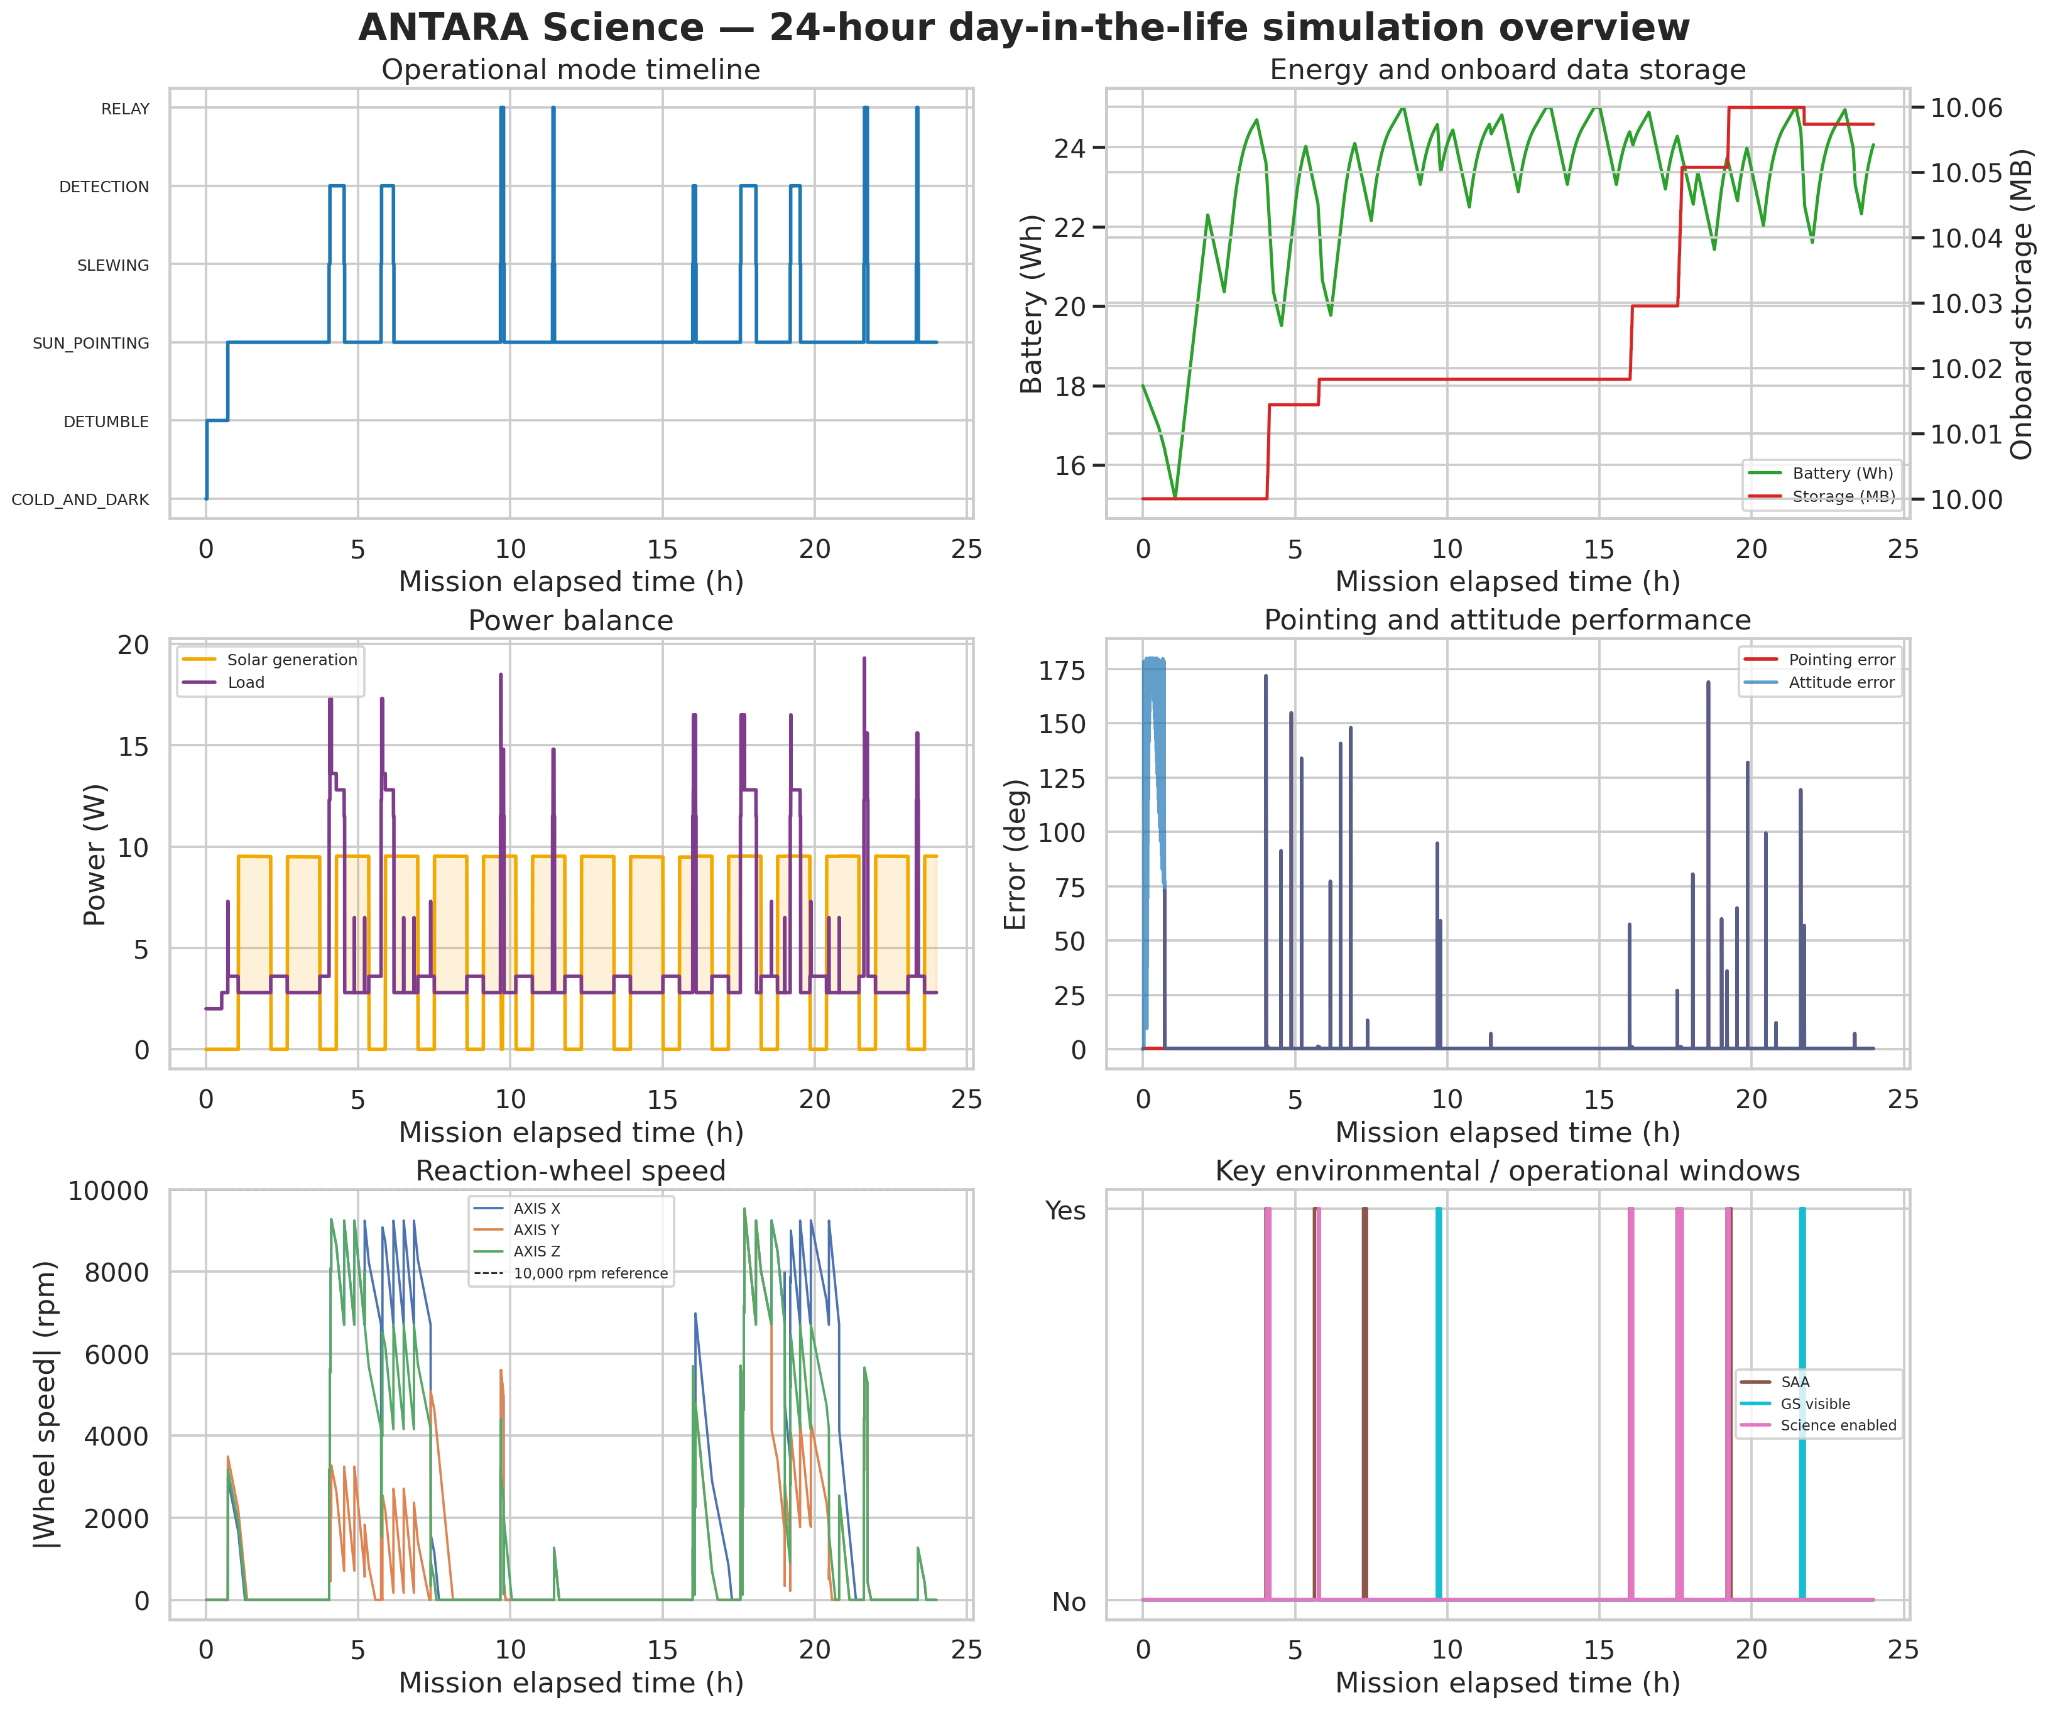
\includegraphics[width=\linewidth,height=0.65\textheight,keepaspectratio]{./media/ditl_overview.png}
\caption{Superseded historical source: 24-hour integrated DITL overview: mode timeline, energy and storage, power, pointing, reaction-wheel speed and operational windows.}\end{figure}


The battery never approaches depletion during this run.

\begin{itemize}
\item
  Initial battery energy is 18.00 Wh
\item
  Minimum battery energy is 15.15 Wh
\item
  Minimum level is approximately 84.2\% of the initial value
\item
  Final battery energy is 24.06 Wh
\item
  Net battery gain over the simulation is approximately 6.06 Wh
\end{itemize}

\textbf{Operational Mode Distribution (24 hours):}

\begin{longtable}{@{}
  >{\raggedright\arraybackslash}p{(\columnwidth - 4\tabcolsep) * \real{0.2991}}
  >{\raggedright\arraybackslash}p{(\columnwidth - 4\tabcolsep) * \real{0.2436}}
  >{\raggedright\arraybackslash}p{(\columnwidth - 4\tabcolsep) * \real{0.4573}}@{}}
\caption{Superseded historical source: 24-hour operational-mode distribution}\\
\toprule\noalign{}
\textbf{Mode} & \textbf{Time Steps} & \textbf{Fraction of Day} \\
Sun Pointing & 37,781 & 87.5\% \\
Detection & 3,134 & 7.3\% \\
Detumble & 1,230 & 2.8\% \\
Slewing & 545 & 1.3\% \\
Relay & 450 & 1.0\% \\
Cold \& Dark & 61 & 0.1\% \\
\midrule\noalign{}
\endhead
\bottomrule\noalign{}
\endlastfoot
\end{longtable}

\textbf{Power and Energy:}

\begin{itemize}
\item
  Average solar generation: 6.05 W
\item
  Minimum battery energy recorded: 15.15 Wh (60.6\% of 25 Wh planning
  capacity)
\item
  No brownouts observed; battery remained above 30\% safety threshold
  throughout the full 24-hour simulation.
\end{itemize}

\textbf{SAA Operations:}

\begin{itemize}
\item
  6 SAA passes observed in 24 hours
\item
  5 of 6 passes achieved active payload science collection
\item
  Total SAA dwell time: \textless2,700 seconds over 24 hours
\item
  Science data generated: 0.060 MB (60 KB) per 24-hour period,
  consistent with 300--400 KB/day (historical estimate, superseded by the v3 sensitivity analysis) estimate at full nominal operations.
\end{itemize}

\textbf{Ground Station Contact:}

\begin{itemize}
\item
  2 contacts with GS1\_India (Goa, 15°N, 74°E) in the 24-hour window
\item
  Contact 1: 368 seconds, maximum elevation 38.5°
\item
  Contact 2: 414 seconds, maximum elevation 77.5°
\item
  Daily downlink capacity at 15--18 kbps (historical, superseded by the ideal 19.2 kbps MCR assumption): \textasciitilde1.5 MB/day ---
  approximately 4× the expected daily science data volume.
\end{itemize}

\textbf{ADCS Performance:}

\begin{itemize}
\item
  Detumble completed in 2,460 seconds from initial body rates of {[}6.0,
  −5.5, 4.5{]} °/s
\item
  18 slew events recorded in 24 hours
\item
  The raw 18-event table gives a minimum slew of 0.442496° (the earlier 5.4° minimum is superseded); the reported maximum is 175.8°; large slews indicate some mode
  transitions require significant attitude manoeuvre time and should be
  factored into operational scheduling.
\end{itemize}

\textbf{Proton Detection (5 active science passes):}

\begin{itemize}
\item
  Historical synthetic FPDU proxy: 50--70\% of the configured AP9-named baseline, not measured detector performance or live AP9
  across all energy channels (5--100 MeV), consistent with partial SAA
  coverage and pitch-angle sampling effects.
\item
  Mean pitch angle ranged 15.6°--77.6° across passes
\item
  Withdrawn count/precision claim: the historical 13,000--108,000 values summed rates without the required time integration. They cannot establish counts or mission-tier precision.
\end{itemize}

\textbf{One-Year Extended Simulation (RAAN 180° baseline):}

\begin{longtable}{@{}
  >{\raggedright\arraybackslash}p{(\columnwidth - 8\tabcolsep) * \real{0.2500}}
  >{\raggedright\arraybackslash}p{(\columnwidth - 8\tabcolsep) * \real{0.1667}}
  >{\raggedright\arraybackslash}p{(\columnwidth - 8\tabcolsep) * \real{0.1282}}
  >{\raggedright\arraybackslash}p{(\columnwidth - 8\tabcolsep) * \real{0.1282}}
  >{\raggedright\arraybackslash}p{(\columnwidth - 8\tabcolsep) * \real{0.3269}}@{}}
\caption{Superseded historical source: Historical standalone campaign statistics; not verified annual integrated Science output}\\
\toprule\noalign{}
\textbf{Metric} & \textbf{Mean} & \textbf{Min} & \textbf{Max} & \textbf{99\% CI} \\
Average Power (W) & 11.22 & 11.19 & 11.25 & 11.16--11.27 \\
Average SOC & 0.987 & 0.986 & 0.987 & 0.986--0.987 \\
Minimum SOC & 0.834 & 0.834 & 0.834 & 0.834--0.834 \\
Battery Cycles & 787 & 785 & 789 & 783--791 \\
\midrule\noalign{}
\endhead
\bottomrule\noalign{}
\endlastfoot
\end{longtable}

\clearpage
\section{Engineering Closure and PDR Entry Conditions}\label{app:source-05}
The MCR establishes a conditional concept and an explicit verification path. The former placeholder-only tables in this appendix are replaced by the evidence dispositions below. No subsystem is assigned a technology-readiness level or margin without a documented basis.

\subsection{Budget Evidence and Limits}
\begin{table}[H]\centering\small
\begin{tabularx}{\linewidth}{@{}p{3cm}p{4cm}X@{}}\toprule
Budget & Current evidence & Closure condition\\\midrule
Mass & 3.0 kg design maximum; 1536.3 g in supplied component entries & Add payload, harness, interfaces and verified quantities; Appendix~\ref{sec:bom-from-upload}\\
Battery & 25 Wh simulation planning capacity & Common load/array configuration and accepted-energy throughput; Appendix~\ref{app:detailed-budgets}\\
Power & RAAN-dependent preliminary predictions & Current electronics load and EOL conditions; no closed FPDU power budget\\
Science / downlink & Provisional 64-bin logical record & Encoding, cadence, loss/quality metadata, storage and scheduled link throughput\\
Payload packaging & 72 mm active length, 2.592 cm$^3$ scintillator & Controlled CAD including gaps, coating, sensors, shield and housing\\
Procurement & Candidate component evidence only & Selected part numbers, interface compatibility and quotations\\\bottomrule
\end{tabularx}\end{table}

\subsection{Verification and Maturation}
Payload qualification requires geometry-matched transport, optics and mixed-species calibration; selected electronics must demonstrate timing, throughput, buffering and measured dead time. Software tests establish accounting only. Integrated acceptance requires runtime/environment manifests, consistent exposure, complete horizons and verified data delivery. Accepted 2026 radiation and RAAN references retain their original identities.

\subsection{Open Decisions and Review Gates}
Payload material, optical isolation, front treatment, optional rear detector, sensor/ASIC/ADC mapping and MCU/FPGA selection remain open. Science owners must approve eligibility, independence and uncertainty definitions while retaining the committed MMSC/MSC/EMSC thresholds. Assignment of named owners and dates belongs to the project review; none is fabricated here. The repository's remaining-decisions register lists the evidence needed for each closure.

\subsection{MCR Exit and PDR Entry}
The MCR establishes a concept, reproducible idealized rate calculations and tested accounting, not calibrated payload performance or mission success. PDR requires controlled interfaces, acquisition timing/throughput evidence, a response campaign and science-coverage acceptance rules. Apply and retest the delivered source patch before new coupled predictions. Long campaigns require separate authorization after bounded verification.

\clearpage

\section{Integrated Mission Simulation and DITL Supporting Analysis}\label{app:ditl-detail}
\subsection{Purpose and Source}\label{app:ditl-source}
The integrated model in \texttt{src/simulations/ditl/ANTARA\_Science\_Sim.py} combines orbit propagation, spacecraft attitude, electrical power, mode transitions, proton-environment assumptions and detector accumulation, and ground-station communications. Its current implementation is a simulation model, not a hardware-in-the-loop qualification system. The shared configuration and individual presets are documented in Appendix~\ref{app:sim-provenance}.
\subsection{Defined Mission Scenarios}\label{app:ditl-preset-details}
The source defines \texttt{leop\_24h}, \texttt{no\_leop\_24h} and \texttt{leop\_1yr}. The first includes Cold and Dark and Detumble; the second begins in Sun Pointing without LEOP startup; the annual scenario includes startup over 8,760 hours. Command-line values may override preset defaults. A comparison of the three scenarios is meaningful only when each output is accompanied by its exact version and configuration.
\subsection{Mode Execution, Time and Energy}\label{app:ditl-accounting}
During startup, detumble and slewing, the simulator uses its fine time cadence. Other operating modes may use a coarser step. Mode occupancy, energy use, detector accumulation and mission elapsed time advance with the same actual integration interval. The corrected exports lack interval-end columns; this audit uses successive timestamps and excludes the endpoint row duration. Explicit interval fields in newer source are not retroactively attributed to these files. Reported fractions should therefore use total elapsed time, not raw row fractions.
The ADCS model retains finite slew and settling requirements, momentum saturation handling and recovery logic. During saturation hold, scientific collection and downlink transmission are inhibited in the documented model. The end of a planned slew duration is not by itself proof of achieved target alignment.
\subsection{Science Data, Detector Statistics and Model Limits}\label{app:ditl-science}
The detector model accumulates expected bin counts and serializes histograms into science data separately. An interval with accepted events need not produce a positive new packet volume until a flush. SAA-exit and simulation-horizon flushes belong to the corresponding pass totals. Bin precision estimates use $1/\sqrt{N}$ for accumulated expected counts, but this does not represent calibrated detector response, stochastic-count realization or a fully validated low-count confidence interval. The environment model's legacy AP9-named variable is a configured baseline and not an independent AP9 computation.
% Generated corrected-evidence block; see registry and audit.
\subsection{Corrected Run Identities and Accounting}\label{app:ditl-evidence}
The authoritative registry binds all 24 files to SHA-256 identities. The corrected daily telemetry contains 7696 and 6553 rows; annual telemetry contains 1434872 rows. All begin at elapsed zero and include the named endpoint. The annual span is exactly 365 days, from 2000-03-01 to 2001-03-01 UTC; the leap day precedes the start. This establishes timestamp coverage, not the missing runtime configuration or hardware validity. The former 50-day truncation finding applies only to superseded inputs.

No duplicate or nonmonotonic telemetry timestamps were found. Day-run timestamp differences are 2/20 s. Annual differences are 2/60 s with one 50 s interval, distinct from the current source default. Annual telemetry has 15161 mode changes versus 16283 transition records and 425 sampled Safe entries. Exact event checks are retained in the JSON audit. The expected adaptive schedule is unknown, so elapsed coverage alone cannot certify that every intended sample was exported. The last sample contributes no additional duration; its native increment fields remain included in cumulative data checks.
\begin{table}[H]\centering\small
\caption{Transition-log versus left-held telemetry mode duration (annual, seconds)}\label{tab:annual-overlap}
\begin{tabularx}{\linewidth}{@{}Xrr@{}}\toprule
Mode & Telemetry & Transitions\\\midrule
COLD\_AND\_DARK & 122 & 120\\
DETECTION & 894,054 & 889,226\\
DETUMBLE & 2,460 & 2,460\\
RELAY & 269,876 & 266,776\\
SAFE & 332,882 & 331,350\\
SLEWING & 375,688 & 620,804\\
SUN\_POINTING & 29,660,918 & 29,425,264\\
\bottomrule\end{tabularx}\end{table}
Transition mode sequence matches: False; timestamp offset range is undefined because the sequences differ. Slew events total 512,586 s across 7928 rows, distinct from 375,688 s Slewing occupancy. These differences require the generating logger/control semantics, not fabricated interval adjustments.
\begin{figure}[H]\centering\includegraphics[width=\linewidth]{evidence/science-ditl/figures/corrected_20261109_day_modes.png}
\caption{Corrected 24-hour mode timelines. Display-sampled points do not define the integration weights.}\label{fig:corrected-day-modes}\end{figure}
\begin{figure}[H]\centering\includegraphics[width=\linewidth]{evidence/science-ditl/figures/corrected_20261109_day_exposure_contacts.png}
\caption{Exposure gates, eligible contact time and native transfer credits for the corrected day runs. Credits are not confirmed ground receipt.}\label{fig:corrected-day-exposure}\end{figure}
\begin{figure}[H]\centering\includegraphics[width=\linewidth]{evidence/science-ditl/figures/corrected_20261109_startup.png}
\caption{Startup and Slewing duration from transition logs, shown separately from telemetry occupancy.}\label{fig:corrected-startup}\end{figure}
\subsection{Annual Exposure, Energy and Native Data}
There are 2346 SAA event records and 2346 sampled SAA windows. Independent science passages additionally require the approved eligibility and quality contract. The acquisition gate totals 247,258 s. Per-pass array sums and telemetry gate-array sums are 3.10842e+09 and 3.10842e+09; these are legacy model expectations, not reconstructed current-instrument events. Bin-wise rate-times-duration comparisons can differ after merging; effective channel metadata and dimensional calibration remain open.

Recorded battery spans 15.097556--25.000000 Wh, ending at 24.019245 Wh. No negative battery row was found. The solar/load integrals are 50288.809/30866.103 Wh under the stated interval convention. Charge efficiency, curtailment and post-step battery semantics prevent treating their difference as stored-energy margin or EOL feasibility.

Native store begins at 10, peaks at 10.005966187, and ends at 10 source MB. Generation minus transfer closes against storage to 7.64e-14 source MB. Histogram-byte totals do not alone establish packet serialization completeness. Raw event packets, lost-event counters and ground-reception archives are absent.
\begin{figure}[H]\centering\includegraphics[width=\linewidth]{evidence/science-ditl/figures/corrected_20261109_annual_exposure_battery_contacts.png}
\caption{Corrected 365-day exposure, battery envelope and contact availability; epoch 2000-03-01. These are recorded model predictions under unresolved runtime configuration.}\label{fig:corrected-annual}\end{figure}
\begin{figure}[H]\centering\includegraphics[width=\linewidth]{evidence/science-ditl/figures/corrected_20261109_annual_modes_cumulative.png}
\caption{Annual telemetry mode occupancy and cumulative geographic versus acquisition-gate exposure. No mission-success classification is inferred.}\label{fig:corrected-annual-modes}\end{figure}
\begin{figure}[H]\centering\includegraphics[width=\linewidth]{evidence/science-ditl/figures/corrected_20261109_annual_native_data.png}
\caption{Daily native generation/transfer and maximum source-labelled store. The historical native packet format is not Science Record v3.}\label{fig:partial-storage}\end{figure}


\subsection{Historical Detumble Summary}\label{app:detumble-evidence}
The supplied 50\,000-row summary reports 16\,133 successful trials and 33\,867 nonconverged trials; all unsuccessful completion times are infinite. Successful-only median, 95th percentile and maximum times are 951.5, 2569.0 and 3026.5~s. Whole-population convergence quantiles and flight reliability are not established. The first baseline row completes in 1009~s, distinct from the integrated 2460~s startup. Initial spin magnitudes range from approximately 0.0008 to 60~deg/s. All rows specify nonzero initial accelerations; the current source rejects that independent-acceleration model, preventing exact reproduction with current code.
\begin{figure}[H]\centering\includegraphics[width=\linewidth]{evidence/detumble/figures/validated_summary.png}
\caption{Historical detumble summary. The empirical completion curve retains all 50\,000 rows as denominator; it is not a censor-adjusted survival estimate. Spin-bin proportions do not establish flight initial-condition probabilities.}\label{fig:detumble-summary}\end{figure}
The summary marks 25\,473 rate-cap hits and records zero peak wheel momentum in every row; neither establishes actuator adequacy. Initial attitude distribution, magnetic field, gains, source revision, random seeds, timeout and failure reasons are missing. No angular-rate or control-effort histories are supplied. Close the generating model and censoring record before bounded timestep, field-orientation, torque/momentum and coupled acquisition validation. Retain reaction wheels plus magnetorquers; no CMG configuration is inferred.

\subsection{Science Record v3 Queue Diagnostic}\label{app:v3-queue}
The corrected sampled-gate workload and outage analysis are in Appendix~\ref{app:science-data-budget}. Native transfer credits above are not v3 records. No arbitrary minimum acquisition duration, count threshold or link derating is introduced. Unknown real acquisition timing and response prevent interpreting the record-slot sensitivity as qualified science delivery.

\clearpage
\section{Additional MCR Study Evidence and Open Decisions}\label{app:new-evidence}
This appendix identifies the new data files supplied for the MCR. The plots and tabulated results are outputs of the supplied study files and do not establish final payload calibration, a new launch epoch, or compliance with spacecraft requirements by themselves.

\subsection{Science grid and mission-tier studies}
The MMSC, MSC and EMSC grid-disposition outputs are based on different cell grids and modeled geographic domains. ``Primary Map'' is the disposition assigned in each output file, not a declaration of global requirement closure. The table summarizes the file contents directly.

\begin{table}[htbp]\centering\small
\caption{Science-map cell dispositions in the supplied studies}\label{tab:new-sci-grids}
\begin{tabular}{lrrrr}\toprule Study & Evaluated & Primary Map & Supplementary & Unclassified \\
\midrule
4-month MMSC & 92 & 92 & 0 & 0 \\
6-month MMSC & 92 & 92 & 0 & 0 \\
12-month MSC & 2020 & 1915 & 105 & 0 \\
14-month MSC & 2020 & 1931 & 89 & 0 \\
extended EMSC & 7940 & 4213 & 3719 & 8 \\
\bottomrule\end{tabular}\end{table}

The MMSC grid file contains 92 modeled cells and the MSC files contain 2020 cells, while the EMSC file contains 7940 cells. These equal the approved polygon-overlap counts at the respective resolutions. They are geometric domains, not automatically eligible science denominators. The missing tier-classification provenance, independent-observation definition and per-channel response still prevent acceptance of the labels as mission success.

\begin{figure}[htbp]\centering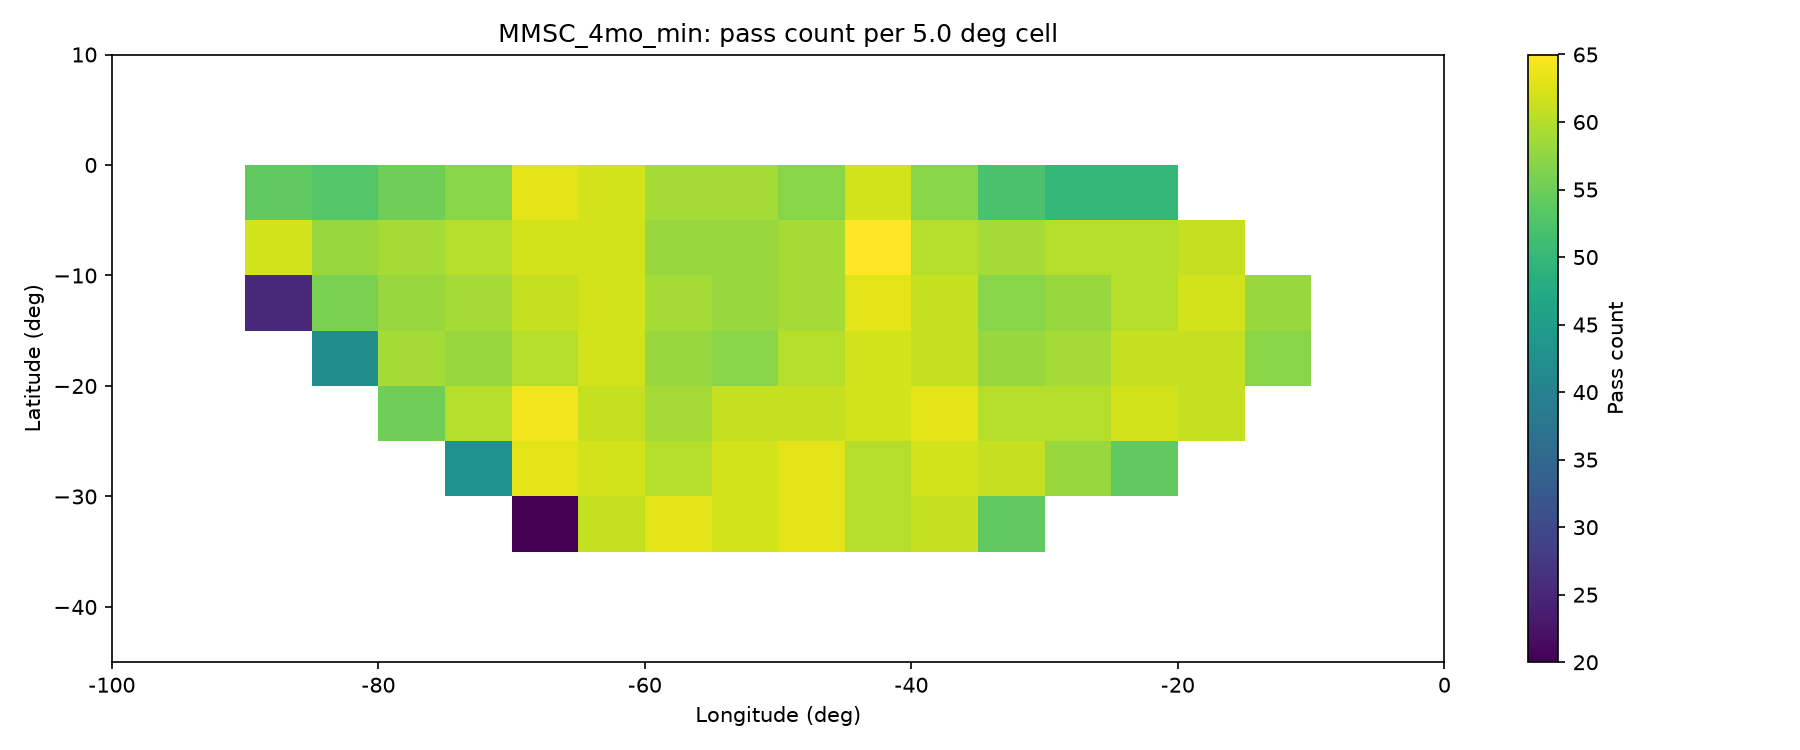
\includegraphics[width=.78\linewidth]{media/mmsc_4mo.png}\caption{Four-month MMSC science-grid output from the supplied simulation archive; model-dependent.}\label{fig:new-mmsc}\end{figure}
\begin{figure}[htbp]\centering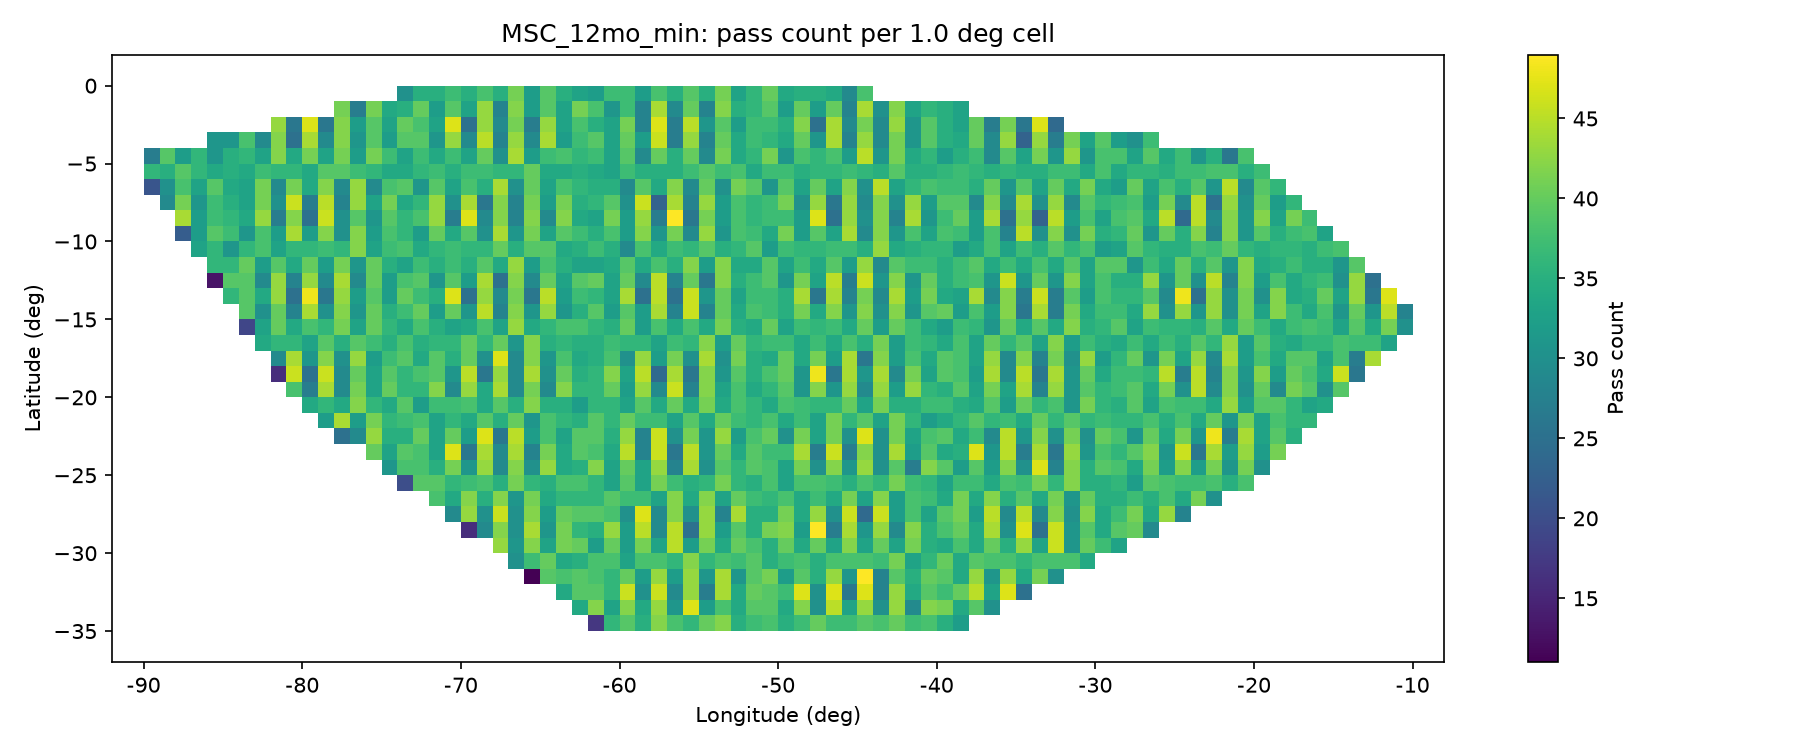
\includegraphics[width=.78\linewidth]{media/msc_12mo.png}\caption{Twelve-month MSC science-grid output from the supplied simulation archive; model-dependent.}\label{fig:new-msc}\end{figure}
\begin{figure}[htbp]\centering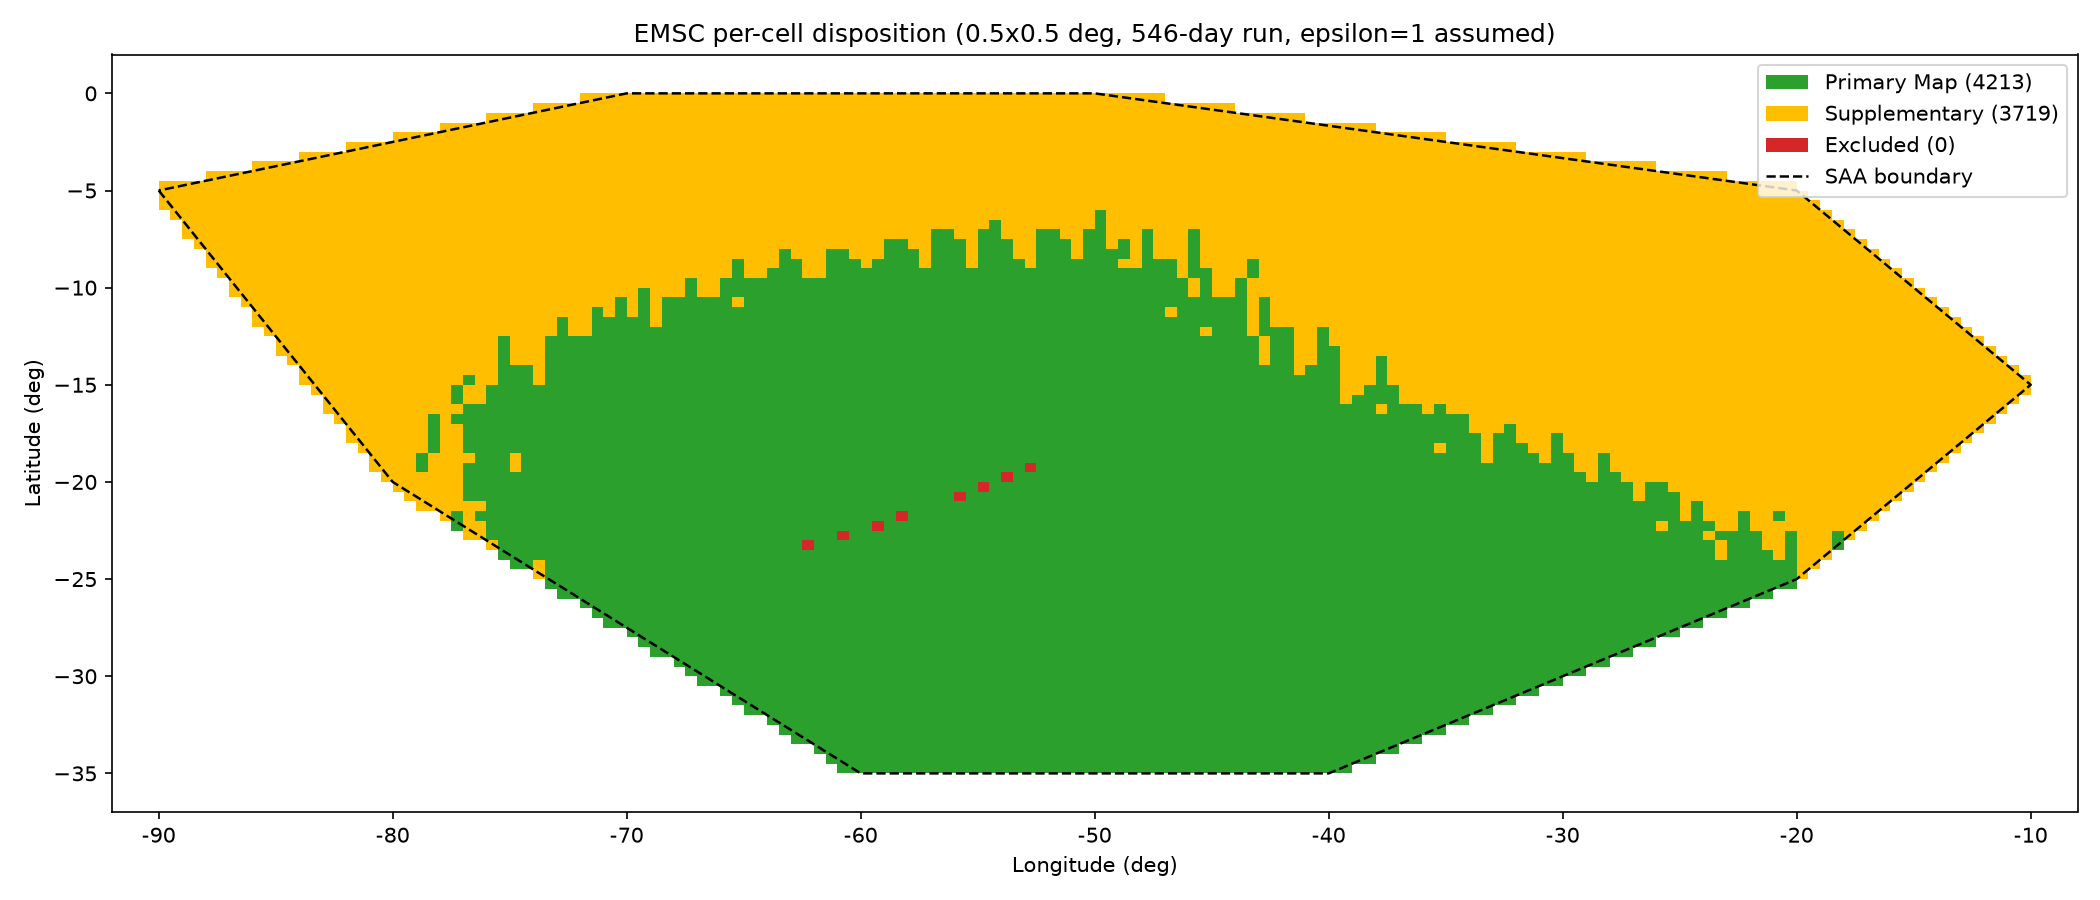
\includegraphics[width=.78\linewidth]{media/emsc.png}\caption{Extended science-grid classification from the supplied simulation archive; model-dependent.}\label{fig:new-emsc}\end{figure}

\subsection{Radiation and detector science model}
The supplied IRENE-related inputs, proton-spectrum output, stopping-range plots and pile-up calculations support preliminary detector analysis. They do not establish a fully calibrated telescope geometry, dead-time limit, response matrix, or actual AP9 output from the integrated Science simulator. The integrated simulator's AP9-named quantity is a configured baseline. Current scintillator dimensions are fixed in Appendix~\ref{app:payload-detail}; accepted event rates and detector response remain unqualified. The supplied 2026 AP9/AE9 grid is reproduced independently and accepted for preliminary 2029 planning with its original epoch retained.
The separate November geometric-factor bundle supports the conditional counting requirements in Appendix~\ref{app:required-g}. Its AP9-labelled 65-threshold spectrum has no generating manifest; the verified date of the earlier AP9/AE9 archive must not be transferred to it. The supplied rate heatmap is an ideal integral-above-5~MeV rate proxy, not a detector-efficiency or required-$G$ map.
\begin{figure}[htbp]\centering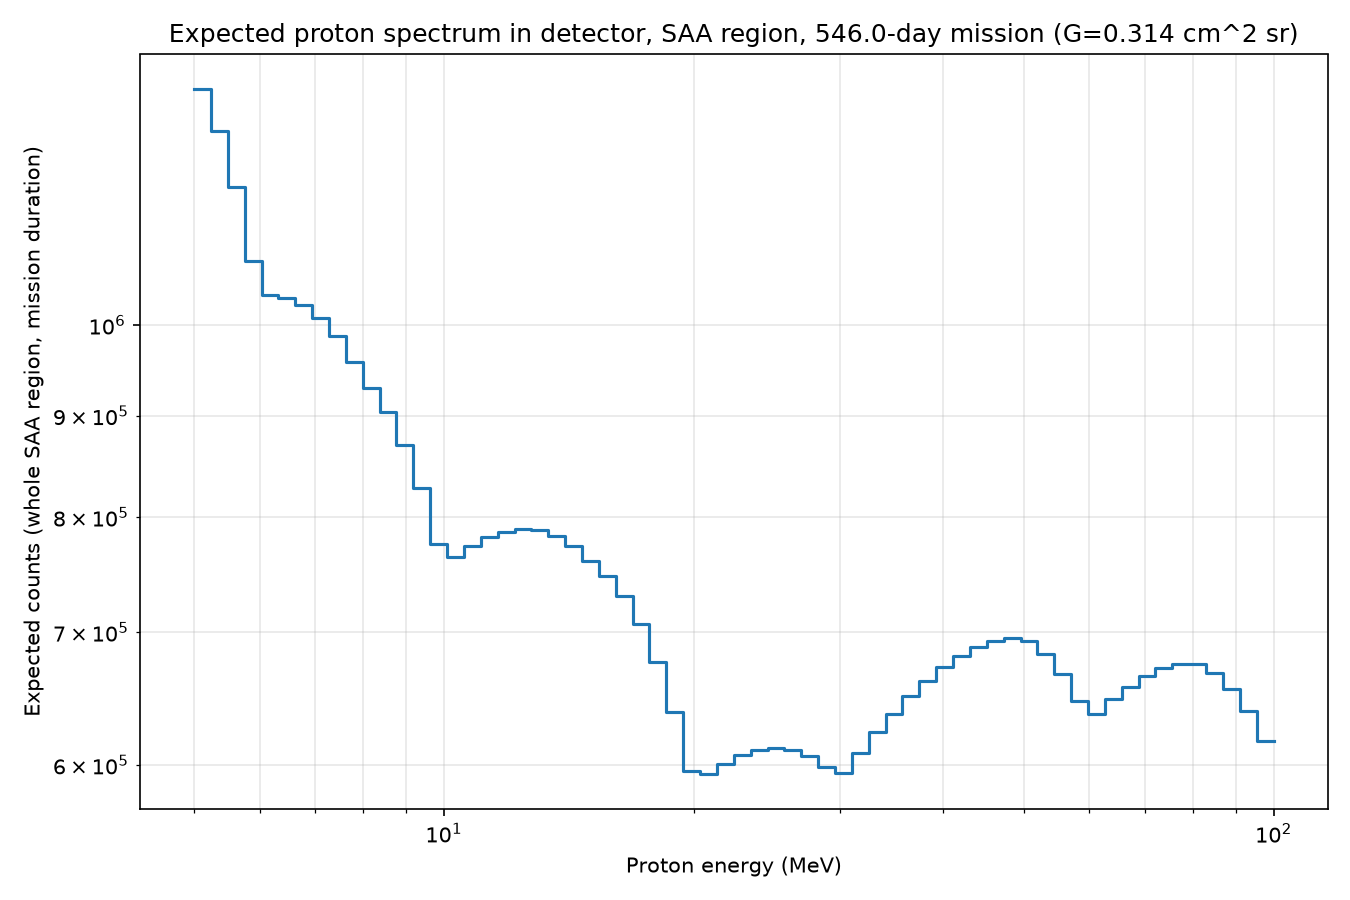
\includegraphics[width=.75\linewidth]{media/spectrum.png}\caption{Historical modeled SAA proton spectrum. Its title assumes 546 days and $G=0.314$~cm$^2$~sr; these labels do not verify runtime duration or connect it to the new unit-$G$ table. This is not a validated detector measurement.}\label{fig:new-spectrum}\end{figure}

\subsection{Ground-station and DITL source files}
The corrected 24-hour and annual exports supersede the earlier incorrect/incomplete Science files. Both day contact logs contain two intervals totaling 766 s. All event origins identify March 2000. Complete recorded horizons do not establish 2029 calibration or current-FPDU qualification. Sections~\ref{sec:sim-leop} and~\ref{app:ditl-detail} contain the regenerated accounting and limitations.

\subsection{Preliminary procurement and mass allocation}
The uploaded bill of materials identifies candidate ADCS, OBC, solar-array, EPS, structure, communications, navigation and antenna parts. The sum of currently specified component-mass entries is 1536.3~g. The payload and deployer-interface hardware do not have mass entries, and the deployable-panel quantity and overall packaging need review. Consequently the bill of materials cannot yet close the mission target of less than 3000~g. Procurement prices remain to be supplied.

\subsection{Manufacturer documentation and CAD inputs}
Manufacturer documents were supplied for the ISISPACE ICEPS2, TensorTech integrated ADCS, GomSpace NanoMind A3200 and NanoCom AX100, 2nd Space CORE/DROP/VERSE hardware and the proposed GNSS components. CAD inputs were supplied for several candidate components. Final mechanical envelopes, actuator configurations, harness allowances and interface drawings must be checked against the actual proposed configuration before the component baselines become final.

\subsection{Remaining verification conditions}\label{sec:new-evidence-open}
\begin{longtable}{p{0.10\linewidth}p{0.47\linewidth}p{0.34\linewidth}}\caption{Open evidence required for MCR closure}\label{tab:new-open}\\\toprule ID & Open item & Needed evidence \\
\midrule\endfirsthead\toprule ID & Open item & Needed evidence \\
\midrule\endhead
O-01 & Reconcile historical SAA counter & New two-run orbit classifications are internally consistent; establish classifier geometry and event definitions \\
O-02 & 2029 campaign identity and RAAN robustness & Runtime manifests and environment timestamps for the team-accepted reference \\
O-03 & Long-term drag and disposal & Verify new 8--10-year cutoff runs, one truncated case, and post-cutoff reentry \\
O-04 & Solar area, efficiency, degradation and EOL margin & Approved solar/EPS report from final configuration \\
O-05 & FPDU response and electronics & Current CAD, optical isolation, transport, timing and mixed-species trigger validation \\
O-06 & Science-tier coverage requirements & Consistent geographic denominator, per-channel uncertainties and pass requirements \\
O-07 & Ground station RF and data-rate closure & Final payload packets, coding, link and antenna design \\
O-08 & Thermal and structural margins & Model outputs checked against component limits; tests planned \\
O-09 & Complete spacecraft mass and cost & Payload, wiring, deployment items, quantities and quotations \\
O-10 & Integrated long-term and scenario verification & Approved output files, code revision and run parameters \\
\bottomrule\end{longtable}

\subsection{Bill of materials, as supplied}\label{sec:bom-from-upload}
The following values are transcribed from the uploaded \texttt{BILL OF MATERIALS.xlsx}. Components are candidates, and none of the unresolved part numbers or interfaces is to be regarded as a final PDR selection. Values of ``TBD'' have not been imputed.
\begin{longtable}{p{0.23\linewidth}p{0.48\linewidth}p{0.08\linewidth}p{0.10\linewidth}}
\caption{Candidate component mass entries from supplied bill of materials}\label{tab:bom-upload}\\
\toprule Subsystem & Component or part & Qty. & Mass (g) \\\midrule\endfirsthead
\toprule Subsystem & Component or part & Qty. & Mass (g) \\\midrule\endhead
ADCS & ADCS-10m  & 1 & 495 \\
OBC & NanoMind A3200 & 1 & 24 \\
Power Generation & Core 1Z & 1 & 114 \\
Power Generation & DROP & 1 & 118 \\
EPS & ICEPS 2S1P+iEPS Battery Type A & 1 & 189 \\
Structure & Verse-03 & 1 & 310 \\
Communications & NanoCom AX100 & 1 & 24.5 \\
Communications & UHF dipole antenna & 1 & 90 \\
Communications & ANT430 & 1 & 30 \\
Deployment & TBD & 1 & TBD \\
Payload & Custom & 1 & TBD \\
Navigation & ZED-F9P-15B & 1 & 1.8 \\
Navigation & AHP54510.07.0100C & 1 & 140 \\
\bottomrule\end{longtable}
The workbook reports a total of 1536.3~g of currently entered masses, before adding the unallocated payload and deployment-interface mass. The current solar-panel quantity entries require confirmation against the intended one fixed and two deployable panel geometry. Costs in the workbook are not quoted amounts.

\subsection{Datasheet alignment checks}\label{sec:databook-check}
The supplied ICEPS2 datasheet describes a 2S1P battery pack with nominal energy 28.8~Wh. The 25~Wh value remains the mission simulation planning capacity. The supplied TensorTech ADCS-10m datasheet explicitly describes a control-moment gyroscope configuration. Since ANTARA intends to use a reaction-wheel and magnetorquer integrated system, that datasheet cannot be treated as proof of the selected ADCS hardware configuration. A matching vendor model and specification must be supplied. The GNSS, radio, antenna, deployment-panel and structure datasheets are candidate mechanical/electrical references, pending interface selection.

\subsection{Approved 2029 Planning Baseline}
\label{app:latest-baseline}
The mission reference is 1 January 2029: 3U, maximum 3.0~kg, approximately 600~km SSO, $97.6^\circ$ inclination, eccentricity approximately 0.001, launch-dependent RAAN, 25~Wh battery planning capacity and reaction wheels with magnetorquers. The team accepts the supplied RAAN data for 2029 planning; the inspected local MCR runtime still starts in 2026, so its generating epoch remains unverified. This does not prevent use as a clearly identified preliminary reference. The supplied radiation map retains its verified 2026 source epoch.

The approved FPDU has five longitudinal main blocks and one front scintillator, eleven SiPMs, no silicon entrance and optional rear detection. Optical isolation, material, calibrated response and processor selection remain open. Appendix~\ref{app:payload-detail} controls current construction and timing. Approximately five years is the operational objective; modeled decay to 300~km and subsequent reentry are separate quantities. The 8--10-year cutoff study retains its configuration and censoring limitations (Appendix~\ref{app:updated-raan}).

\clearpage
\section{Updated RAAN Trade and Orbital Decay Evidence}\label{app:updated-raan}
This appendix transcribes the four latest supplied MCR campaign CSV files: \path{raan_master_trade_matrix(1).csv}, \path{mission_statistics(1).csv}, \path{drag_lifetime_analysis(1).csv}, and \path{orbit_classification(1).csv}. These outputs are the newest \emph{provisional} trade-study evidence, not an integrated DITL rerun or a flight-verified performance guarantee. The approved mission analysis epoch is 1 January 2029; the supplied CSV files alone do not prove that they were generated with that epoch or with the final 3~kg spacecraft model.

\subsection{RAAN trade-study summary}
\begin{table}[htbp]\centering\footnotesize
\caption{Latest RAAN trade matrix, as provided. SOC is expressed as a percentage of capacity; the minimum column averages run minima, not the worst sample; orbit counts are sums across the study runs, not annual values.}\label{tab:raan-updated}
\begin{tabular}{@{}rrrrrrr@{}}\toprule
RAAN & Power (W) & Mean SOC (\%) & Mean min. (\%) & Life (yr) & SAA-only & GS-only\\\midrule
$0^\circ$ & 11.02 & 97.9 & 69.6 & 9.46 & 79,377 & 11,536 \\
$30^\circ$ & 10.82 & 97.2 & 74.7 & 9.53 & 79,865 & 11,613 \\
$60^\circ$ & 10.28 & 95.1 & 70.4 & 8.95 & 74,917 & 10,995 \\
$90^\circ$ & 10.13 & 94.9 & 72.7 & 8.88 & 74,340 & 10,969 \\
$120^\circ$ & 9.02 & 88.1 & 54.4 & 8.23 & 69,267 & 10,196 \\
$150^\circ$ & 9.50 & 92.7 & 71.6 & 8.66 & 72,819 & 10,657 \\
$180^\circ$ & 11.17 & 98.2 & 73.4 & 8.58 & 72,103 & 10,498 \\
\bottomrule\end{tabular}\end{table}
The sampled RAAN set is $0^\circ,30^\circ,60^\circ,90^\circ,120^\circ,150^\circ,180^\circ$. The largest tabulated mean generated power is 11.17~W at $180^\circ$; the smallest is 9.02~W at $120^\circ$. The latter has the lowest mean of run-minimum SOC (54.4\%). Consequently the current study does \emph{not} justify naming $0^\circ$ or $30^\circ$ universally optimal. The choice of RAAN is launch-dependent; a robust spacecraft must be assessed across its feasible orbital-insertion cases. The RAAN matrix does not by itself demonstrate the fully integrated power/attitude/communications performance of a final 2029 mission.

\subsection{Orbit-classification bookkeeping}
The raw classification table contains 685798 rows: seven RAAN values and two recorded runs per RAAN. The entries in the RAAN trade matrix match the summed counts of \texttt{QUIET}, \texttt{ONLY\_GS}, \texttt{ONLY\_SAA} and \texttt{MIXED} orbit classes in that source file. \texttt{orbit\_number} is unique within each RAAN/run pair. Classifications are mutually exclusive for each orbit record, but the tabulated counts pool both runs and therefore must not be presented as a one-year orbit count. The modeled classifier and event geometry still require documentation before they can be used as physical detector-on SAA passes or real GS contacts.

\subsection{Lifetime to the modeled 300 km cutoff}
\begin{table}[htbp]\centering\small
\caption{Two drag-study records per RAAN. Time is to termination of the supplied integration; the listed endpoint is not atmospheric reentry.}\label{tab:drag-updated}
\begin{tabular}{@{}lrr@{}}\toprule RAAN & Recorded time (yr), range & Endpoint altitude (km), range\\\midrule
$0^\circ$ & 8.96--9.96 & 299.9--299.9 \\
$30^\circ$ & 9.06--9.99 & 299.9--334.9 \\
$60^\circ$ & 8.87--9.04 & 300.0--300.0 \\
$90^\circ$ & 8.86--8.90 & 299.6--299.8 \\
$120^\circ$ & 8.23--8.24 & 300.0--300.0 \\
$150^\circ$ & 8.53--8.79 & 299.9--299.9 \\
$180^\circ$ & 8.33--8.83 & 299.9--299.9 \\
\bottomrule\end{tabular}\end{table}
Across the 14 records, modeled termination times span 8.23--9.99 years. Thirteen rows terminate near 300~km. The remaining $30^\circ$ record terminates at 334.93~km after approximately 9.99~years, so it cannot be counted as a completed decay-to-300-km result. This suggests an approximately 8--10-year decay timescale \emph{under these study assumptions}, not proof of the earlier five-year orbital-decay estimate. The output includes no post-300-km propagation to an atmospheric reentry condition. Atmospheric model, ballistic coefficient, starting epoch, mass, attitude-dependent area, solar activity, termination cause and parameter uncertainty require source-code provenance review. These results are preliminary and do not establish disposal compliance.

\subsection{Monte Carlo statistics: scope and interpretation}
The provided \path{mission_statistics(1).csv} corresponds numerically to the $180^\circ$ RAAN row for average power (11.17485~W), mean SOC (0.98234), mean run-minimum SOC (0.73446), cycle count (6565.43) and lifetime (8.58241~years). Its confidence intervals should not be interpreted as 99\% population coverage without verification of the statistical method and independent sample count; the raw study includes only two runs per RAAN. The power and lifetime fields represent modeled quantities, not measured solar electrical output or a verified physical lifetime.

\subsection{Design implication for the MCR}
The operational science campaign targets a roughly five-year mission, while the newest drag study points toward a potentially longer residence time before reaching 300~km. These statements are not interchangeable. The MCR should maintain the five-year \emph{operational objective} while qualifying the uncertain passive decay and post-mission disposal timeline. Detailed DITL operations are being rerun separately; their future results should be incorporated with independent identification of date, simulation revision and model assumptions.


\end{document}
